\documentclass[table,xcdraw]{article}

\usepackage{tocloft}
\usepackage{appendix}
%\usepackage[title,titletoc]{appendix}
\usepackage[euler]{textgreek}
\usepackage{upgreek}
\usepackage{gensymb}

% Vertical spacing before Table of Contents
\usepackage{blindtext}
\setlength{\cftbeforetoctitleskip}{-50pt}
% \setlength{\cftaftertoctitleskip}{0pt}

\renewcommand{\contentsname}{Table of Contents}
%\renewcommand{\bibname}{Bibliography}
\renewcommand{\appendixname}{Appendix}
%\renewcommand{\cftchapleader}{\cftdotfill{\cftsecdotsep}}
\renewcommand{\cftsecleader}{\cftdotfill{\cftsecdotsep}}
\renewcommand\cftsecdotsep{\cftdot}
\renewcommand\cftsubsecdotsep{\cftdot}


\setlength\parindent{0pt}

\usepackage[utf8]{inputenc}
\usepackage[a4paper, total={6in, 8in}]{geometry}
\usepackage{hyperref}

%packages for svg images
\usepackage{svg}

\usepackage{amsmath}
\usepackage{amsfonts}
\usepackage{amssymb}
\usepackage{float}
\usepackage{caption}
\usepackage{subcaption}
%\usepackage[usenames,dvipsnames]{color} % color text
\usepackage{svg}

\usepackage{listings}
\usepackage{alphalph}
\usepackage{hyperref}
\hypersetup{
    colorlinks=true,
    linkcolor=blue,
    filecolor=magenta,      
    urlcolor=blue,
    pdftitle={SM_MP_2b},
    bookmarks=true,
    pdfpagemode=FullScreen,
    }
    
    
\usepackage{graphicx}
%\usepackage[table,xcdraw]{xcolor}

%% No orphan or widow lines
\clubpenalties 3 1001 1002 1003
\widowpenalties 3 2001 2002 2003

%% Header
\usepackage{fancyhdr}
\pagestyle{fancy}
\setlength\headheight{26pt} %% just to make warning go away. Adjust the value after looking into the warning.
\rhead{
\includegraphics[width=3.0cm]{han_logo.jpeg}}
%%

% Vertical spacing before every new chapter
\usepackage{titlesec}
\titleformat{\chapter}[display]
{\normalfont\huge\bfseries}{\chaptertitlename\ \thechapter}{20pt}{\Huge}   
\titlespacing*{\chapter}{0pt}{-50pt}{10pt}

\title{SM Minor Project 2b}
\author{}
\date{October 2020}

%% BIBLIOGRAPHY PACKAGES %%%%%%%%
\usepackage{filecontents}
\usepackage[
hyperref=true,
firstinits=true, % render first and middle names as initials
maxcitenames=3,
maxbibnames=99,
style=authoryear,
dashed=false, % re-print recurring author names in bibliography
natbib=true,
useprefix=true, % for inclusion of 'de' 'da' in surname
urldate=long,
backend=biber,
uniquename=false,
style=apa
]{biblatex}

% No unit separator after publication year:
\usepackage{xpatch}\xapptobibmacro{date+extrayear}{\nopunct}{}{}

% No month for publication year:
\AtEveryBibitem{\clearfield{month}}

% Use single quotes around titles:
\usepackage[british]{babel}
\usepackage{csquotes}

\DeclareNameAlias{author}{last-first}
%\renewcommand*{\mkbibnamefirst}[1]{{\let~\,#1}} % insert thin spaces between author initials
%\renewcommand*{\bibnamedelimd}{\addlpthinspace} % insert thin spaces between author initials
\renewcommand*{\bibinitdelim}{} % no spaces between author initials (requires biber)
\renewcommand*{\nameyeardelim}{\addcomma\addspace} % insert a comma between author and year in-text citations
\renewcommand*{\newunitpunct}{\addcomma\addspace} % comma as separator in bibliography, not full stop
\renewbibmacro{in:}{} % remove 'in:' preceding article title

% Place volume number within parentheses:
\renewbibmacro*{volume+number+eid}{%
    \printfield{volume}%
    \setunit*{\addnbspace}% NEW (optional); there's also \addnbthinspace
    \printfield{number}%
    \setunit{\addcomma\space}%
    \printfield{eid}}
\DeclareFieldFormat[article]{number}{\mkbibparens{#1}}

% Spacing in bibliography:
\setlength{\bibitemsep}{12pt}
\setlength{\bibhang}{16pt}% the hanging indent

\DeclareFieldFormat{year}{\mkbibparens{#1}}
\DeclareFieldFormat{type}{\mkbibbrackets{#1}}
\DeclareFieldFormat{url}{Available at: \url{#1}}

\addbibresource{references.bib}
%%%%%%%%%%%%%%%%%%%%%%%%%%%%%%%%%%%

\begin{document}

%% COVERPAGE %%%%%%%%%%%%%%%%%%%%%%%%%%%%%%%%%%%

\begin{minipage}{\linewidth}
	\begin{flushright}
			\textbf{HAN MASTER MAJOR PROJECT}\\
	\end{flushright}
			\vspace{20pt}
	\begin{center}
			\LARGE\textbf{Deployment of a Time-Triggered Architecture schedule for a fully redundant Real-Time Embedded System with MATLAB-Simulink}\\
	\end{center}
	\vspace{5pt}
    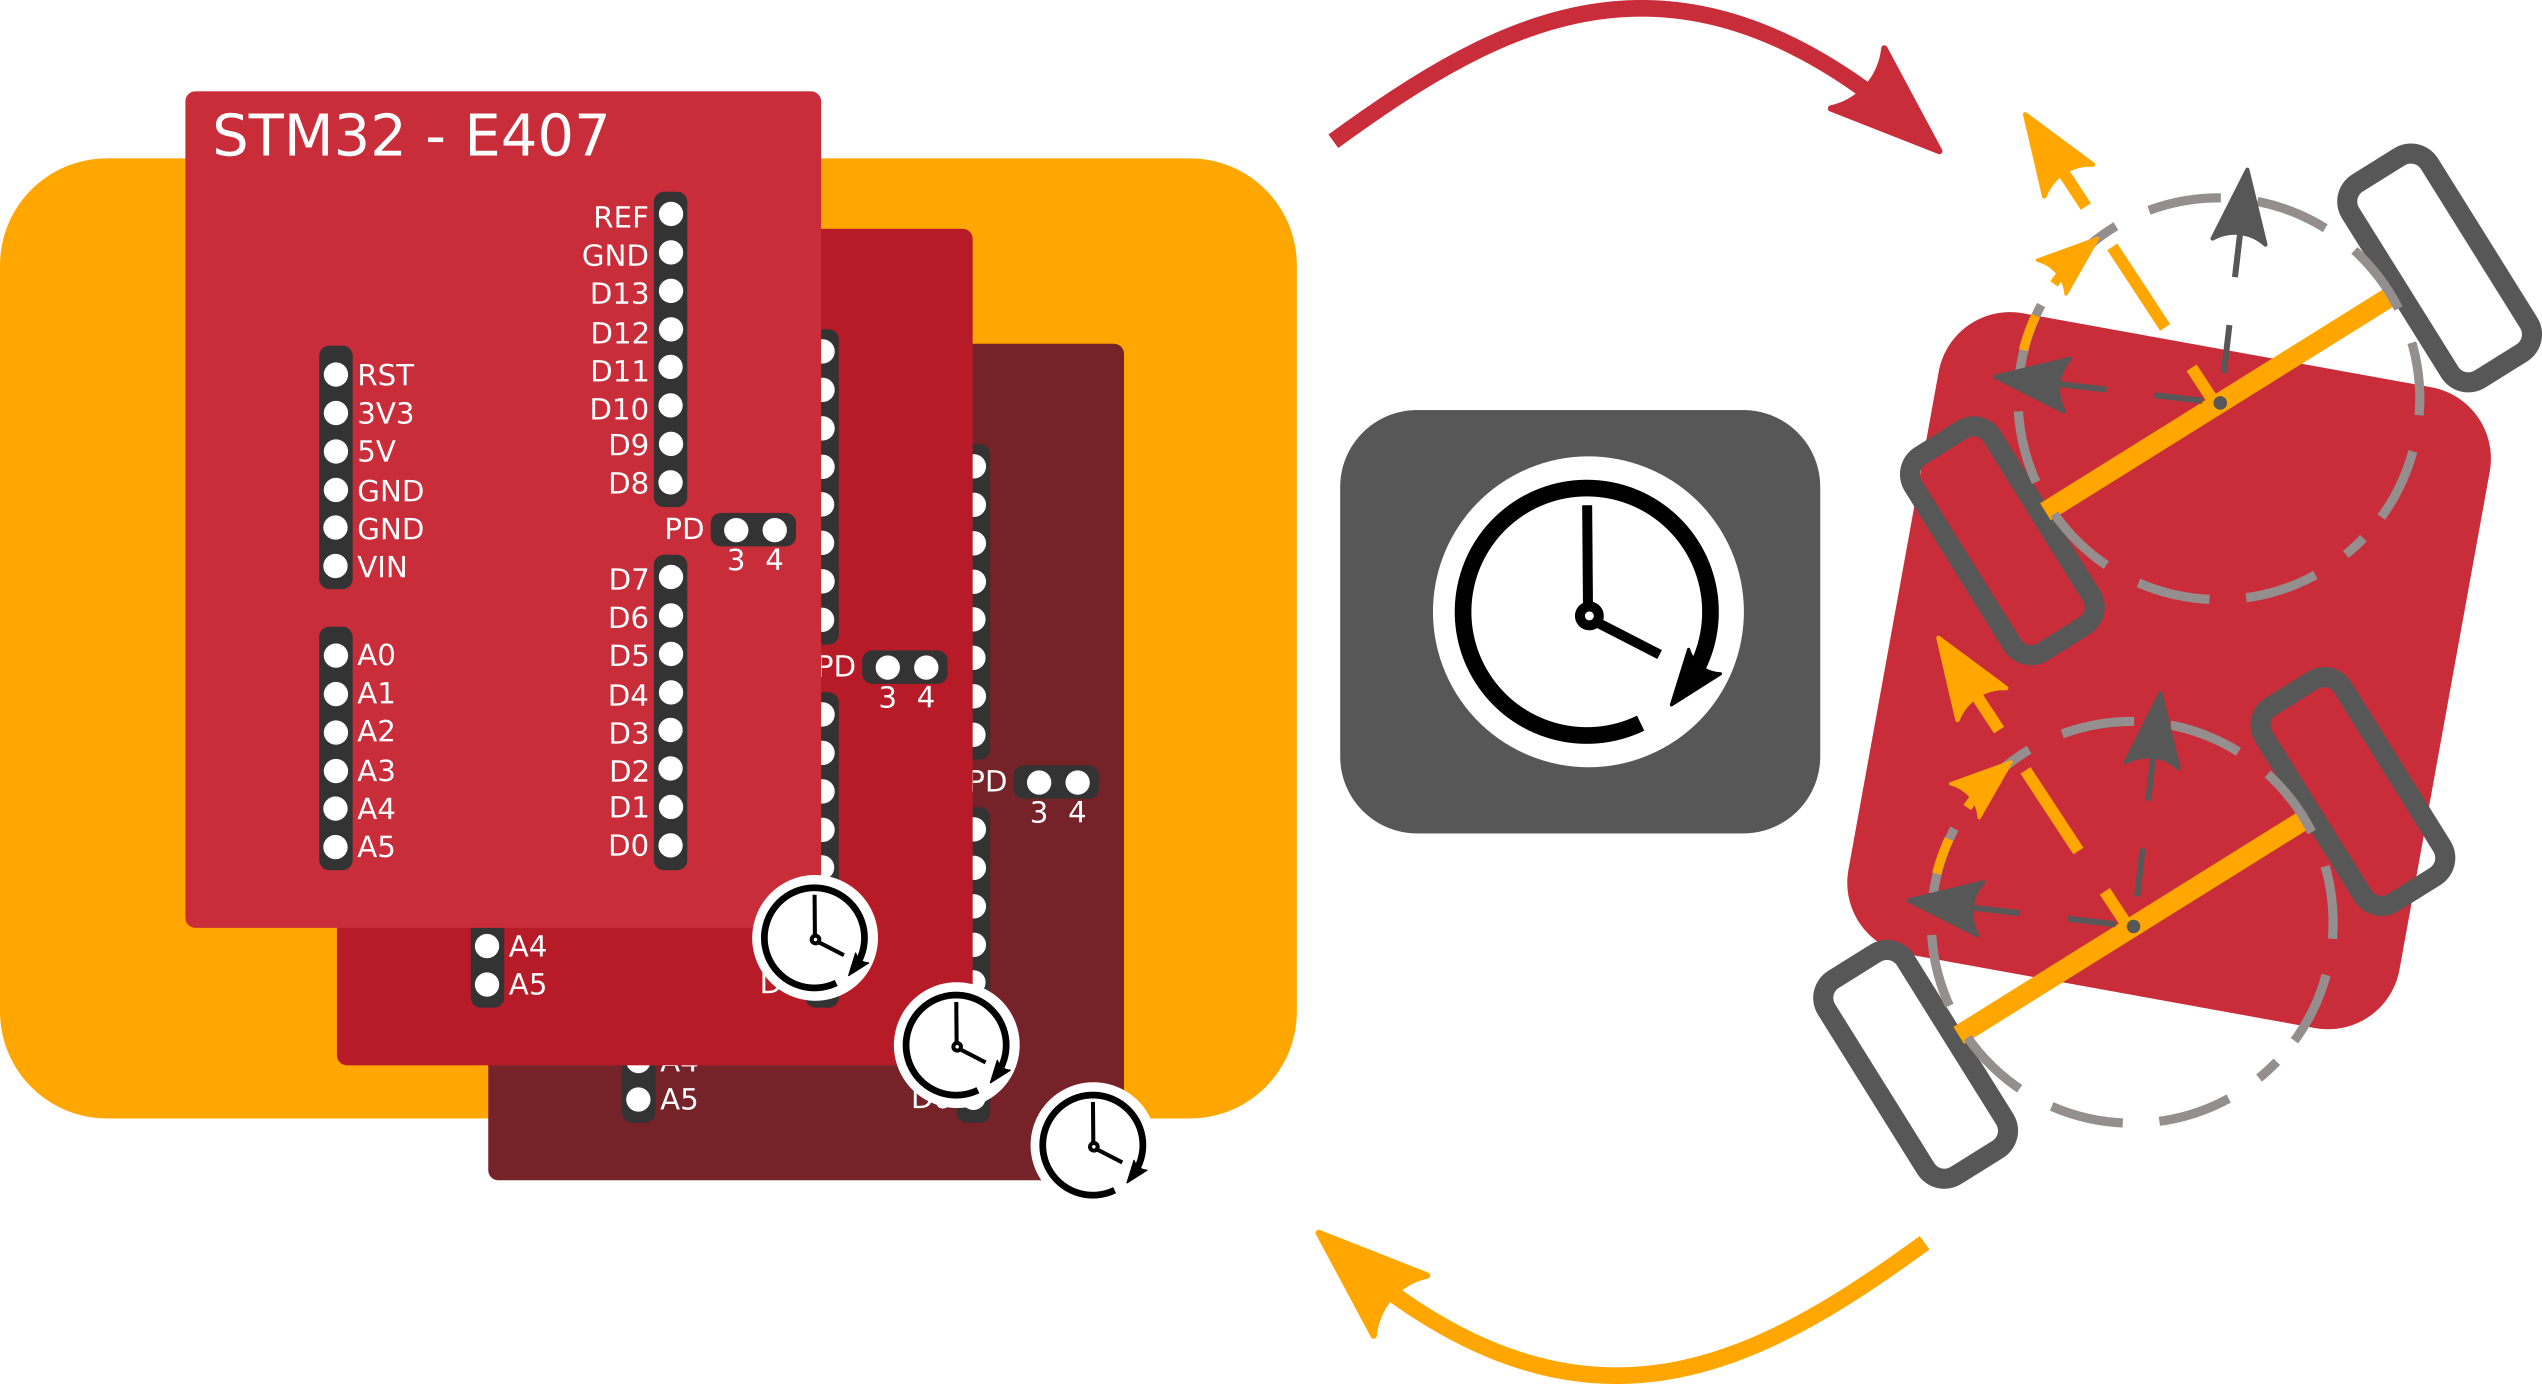
\includegraphics[width = \linewidth]{figures/frontmatter.png}
	\vspace{5pt}
	\begin{center}
			\Large{Diego Martín López \quad 659292\\}
			
%			\\Date: \today
            \vspace{20pt}
            \Large\textbf{
			\\Company supervisor: Aart-Jan de Graaf \textendash lector Meet- en Regeltechniek
			\\HAN supervisor: Sanket Dutta \textendash researcher at HAN
			\vspace{5pt}
			\\Arnhem, 2$^{nd}$ of February 2022}
	\end{center}
	\vspace{30pt}
% 	\begin{flushright}
% 	        \large{20$^{th}$ of January 2022 -  v.3.2}
% 	\end{flushright}
\end{minipage}

\pagenumbering{gobble}
% \pagenumbering{roman}
% \footnotetext[0]{template minor project report}

%%%%%%%%%%%%%%%%%%%%%%%%%%%%%%%%%%%%%%%%%%%%%%%%

\newpage

%% SUMMARY %%%%%%%%%%%%%%%%%%%%%%%%%%%%%%%%%%%%

{\Large\textsc{Summary}}\\

% To complete your master program, of course you want to present an impressive Master Major Project report. Still, it can appear quite a struggle to accomplish this. To provide a helping hand, this document is provided. 
% Its objective is twofold. It provides some background and tips how to create a well written Master project report, and this word document itself serves as template are expected to use as a default to create your own report.

% When you compose the summary of your report, consider it a separate document, very briefly presenting your complete project. Probably, your summary will be read by many more people than the body of your report. And a well-written summary may make people decide to read your full report. So time spent on your summary is generally well invested. 

% A simple way of reducing your message to the nitty-gritty of a summary, is to ask a colleague to interview on your major project topic. Record (on your cell phone) the answers you give to “what did you research, why, how did you tackle the research question, what did you find and what are the conclusions and implications?”  Next, type out the sentences. 


% [6] Report writing for readers with little time: chapter 6.4 (summary)

% What is this project for?
This project aims to prove that it is possible to develop and deploy a Real-Time distributed controller using HANcoder, an extension of \textsc{Matlab}-Simulink developed by the HAN. This is an interesting topic for the HAN's embedded system department as they can use the findings of this thesis as educational material for the Master in Engineering Systems Embedded Systems (MES-ES) module. It is also interesting to develop a tool that allows building Real-Time embedded applications within the HANcoder environment as this will open up a new field of projects to develop.\\

% Main ideas on how and previous work
The test case chosen to be developed as a template model focuses on a Time-Triggered architecture schedule for a fully redundant embedded controller for a two-axle vehicle. The embedded systems department already had research done regarding this topic and the Minor Project from the course 2021 in the MES-ES module set the foundation on generating global time in an ensemble of boards using the CAN communication protocol. This project follows up from both pieces of research and combines them developing the controller for a three boards ensemble, so triple modular redundancy can be performed over the output signals to the vehicle.\\

% Focus on how (1): TTA schedule first basic cycle
The Time-Triggered schedule is divided into two basic cycles. The first basic cycle's purpose is to ensure that the boards are synchronized and to set the time master of the ensemble. In an ensemble of boards it is important to set a global time so all the components in the system follow the same time frame. During the first basic cycle the three boards vote which of them should be the time master of the ensemble, i.e. in charge of setting the global time. To improve redundancy the communication between the boards is done using two CAN channels sending the same information. Every message is also transmitted several times during the same communication task to improve the chances of being received.\\

% Focus on how (2): TTA schedule second basic cycle
 The second basic cycle of the Time-Triggered schedule is devoted to perform the controller calculations. Apart from the controller boards, the test case system is compounded of two more boards: one to generate the input signal and the other as a vehicle emulator. The controller receives the steering and speed signals from the input generator and the wheel displacement from the vehicle emulator. Then the three controller boards make the same calculations to generate the new torque for the vehicle wheels according to the input signals and their current state. The two controller boards that are not acting as time master send their respective calculations in two separate communication tasks so that the master can assess their validity. With the triple modular redundancy the master checks whether the three signals agree or not. As long as two signals agree, the output is considered valid and sent to the vehicle emulator.\\

% Results and discussion
The Real-Time embedded controller has been successfully developed and deployed. The vehicle emulator has been observed to follow the input generator signal with a PID controller of $50\,$ms cycle time. This proves that the concept is feasible and functional. However, there are three main issues regarding time constraints and communication that limit the prototype's potential. Firstly, there are missing messages during the boards' communication exchange. While the boards are synchronized, it has been observed that some messages are not received by all other boards. Secondly, there is a high computational load during message transmission, so the system cannot run with a faster execution time. Lastly, the current time master election policy requires a lot of time thus it is advised to optimize this procedure. Saving up time in the presented controller operations is key to allow for more complex projects to use the research of this thesis.\\

%%%%%%%%%%%%%%%%%%%%%%%%%%%%%%%%%%%%%%%%%%%%%%%

\newpage

%% TABLE OF CONTENTS %%%%%%%%%%%%%%%%%%%%%%%%%%

\tableofcontents
%\addcontentsline{toc}{section}{\protect\numberline{}Table of Contents}%

%%%%%%%%%%%%%%%%%%%%%%%%%%%%%%%%%%%%%%%%%%%%%%%

\newpage
\pagenumbering{arabic}

\section{Introduction}
%% Brief introduction's introduction
This project aims to develop and deploy an embedded controller for a two-axle vehicle within the \textsc{Matlab}-Simulink environment. The focus of the project lays on the temporal aspects of the controller, mainly cycle time, ensemble precision and temporal control. This is done to prove that it is possible to control a vehicle using this methodology and to finish a software ready for further study, for both education and research. The temporal part of the software is designed in such a way that it is possible to build and design different Real-Time applications upon it using \textsc{Matlab}-Simulink. In the next sections, this topic is introduced step by step.

\subsection{Background}
% Provide a general description of the context of the problem and why it requires attention. The first sentences should introduce the subject of your Project. As the reader is not aware of the context of your work, you need to present some backgrounds on your project. In what kind of industry is your work relevant? What is the origin of your project? What is the scope of your project? If you use other sources to write the introduction, refer to these sources when you state ideas or other remarks that you have drawn from these other sources.

% Common pitfalls:
% \begin{itemize}
%     \item Don’t use the background to extensively present the company or organization you work for. For the companies number of employees, product range and financial results see chapter 2.6.
%     \item It is always difficult to decide how much background needs to be added. It could help if you imagine you are writing the report for a fellow master student (also working on his or her final project) that does not know about your specific topic. 
% \end{itemize}

%% Context of the problem
%  Model-based design and software
%%% TO DO: Proper introduction to the topic!! We need to flow better towards the next sentence. Maybe start with some time trigger vehicle controller stuff, or robustness using Time-Triggered schedules.
Distributed embedded systems popularity is rising as computer power becomes stronger and cheaper. When designing an application for any field that involves some risk, either on users or products, safety is a very important requirement. One way of achieving safety is by obtaining robustness with redundancy, in other words, having more than one point where the system can fail, so another part of the system can take over and resume operations. Embedded controllers rely on this idea, that is why several processors are temporally synchronized and merged in an ensemble with several failure points.
% In what industry is my work relevant?
The HAN embedded systems department is particularly interested in developing this technology using \textsc{Matlab}-Simulink, concretely HANcoder, which is an extension of Simulink developed by the HAN. This is because this platform is being used for both educational purposes and research.\\

Embedded system projects usually require an interdisciplinary background. A software design methodology that helps with department communication and system integration is model-based design \citep{modeling_languages_rtes}. Embedding software has traditionally required specific text programming (usually using C) based on some previously designed specification. However, model-based design is becoming more popular as an alternative. In this other method programming blocks are joined together in a model directly resembling the specification. HAN University of Applied Sciences has developed extra layers of functionality over \textsc{Matlab}-Simulink with HANcoder and HANTune, which provide blocks for, among others, Controller Area Network (CAN) communication, and allow for hardware in the loop testing, respectively. This helps in speeding up the development process flashing the embedded software onto the hardware and allowing for fast prototyping.\\

%% Why it requires attention
After rigorous research, it has been found that Real-Time Embedded Systems (RTES) development with \textsc{Matlab}-Simulink is either based on simulation or lacks some key features we consider important, such as external clock activation or global time establishment over a distributed system. When dealing with an ensemble of boards that have to be synchronized, it is important that all the boards run their programs with the same \textit{time} or rhythm, which is called granularity. There is a limit of 10 kHz on \textsc{Matlab} software granularity and no built-in option for execution under a hardware clock interruption basis has been found. This latter would allow for the granularity to be set by an external clock. The STM32-E407 boards employed in this project are also not part of the supported hardware by the official source \citep{embedded_simulink_supported_hardware}. There is some work done regarding scheduling with a \textsc{Matlab} toolbox described in \citep{Torsche_1} or \citep{Torsche_2} and for Linux target RTES, as can be seen in \citep{Matlab_RTE_Linux}, but there is no deployment on any STM32 boards (apart from the discovery series). There are also no flexible proposals to develop Real-Time distributed applications with a hardware clock synchronization. The work proposed in this project plan will develop some tools to cover these functionalities to solve a technological problem and thus allow for further development works with HANcoder on Real-Time distributed applications.\\


%% Origin of the project
%% Introduce the subject of your project
This Major Project does not start from scratch, as it is based upon the Minor Project of the embedded systems module of the Master of Engineering Systems at the HAN. The Minor Project for the embedded systems module proposed the development of a two-axle vehicle controller within a fully redundant context using \textsc{Matlab}-Simulink and HANcoder. More information about the two-axle vehicle is presented later in section \ref{sec:two_axle_veh_spec}. The controller, including the motion controller and the motion estimator, processes the signals from the input generator towards the vehicle emulator, as presented in figure (\ref{fig:control_structure}). However, there seems to be no evidence yet that a Real-Time distributed controller can be actually programmed within the \textsc{Matlab}-Simulink and HANcoder environments. The initial version of the software allowed for Time-Triggered message communication among three STM32-E407 boards using CAN with time master voting logic in the ensemble. This Major Project focuses on the latest phases of the Minor Project proposal, building upon the initial version of the software and including deployment of the controller.\\

\begin{figure}[h!]
    \centering
    \includegraphics[scale=0.45]{figures/introduction/controller_overview.pdf}
    \caption{High-Level Overview of the Control Structure. The blue box encircles the controller functionality. This figure was taken from the Minor Project description in the embedded systems module.}
    \label{fig:control_structure}
\end{figure}

% Introduce some important ideas of embedded systems
 There are two important aspects already implemented in the Minor Project that help in the robustness of the Major Project development. Using a Time-Triggered schedule requires thinking prior to software execution when every different task of the program shall be executed. This makes the design more complex but allows the controller to have a deterministic behaviour. The choice of using three boards allows to use triple modular redundancy in later phases of development. This is used during this project for the value domain (the controller calculations) to ensure that, even if one of the three calculations from the boards (one calculation per board) is incorrect, there are two calculations that are consistent with each other. These two ideas are further explored and explained in chapter \ref{sec:methodology}.\\

%% Scope of the project
The controller will not be deployed in a real car but it will just be tested under a computer simulation, with the controller fully deployed within several STM32-E407 boards. The signals input to the controller and processed by it will be managed by computer emulators. The different components of the system already exist in a \textsc{Matlab}-Simulink program without temporal elements taken into account. The project focuses on (1) the development of a time synchronization software that can be used as a template in the future for further development of RTES, (2) the adaptation of the already existing software of the signal generator, controller and vehicle emulator to fit within the time synchronization software framework and (3) the deployment of the whole system in an ensemble of boards, using a test case to demonstrate that the software is able to control a two-axle vehicle. The test case is studied and analysed exploring the different scenarios where failures could happen (using fault injection) and either visualizing or recording the states of the different variables (monitoring).\\



%%%%%%%%%%%%%%%%%%%%%%%%%%%%%%%%%%%%%%%%%
\subsection{Problem definition}\label{sec:problem_definition}
% Now we know the background, what is exactly the problem you face? Try to pinpoint the problem by an accurate definition. This is the most difficult and at the same time most important part of your report. Make sure you take sufficient time to think about this! Graphs presenting components, connecting signals and flows might be helpful here. The problem definition as discussed in the course Introduction Modeling provides a structure. And don’t forget to introduce names and units!

%% We have to define the problem!!
As already stated in the previous chapter, no evidence has been found that a Real-Time Time-Triggered fully redundant controller can be deployed in STM32-E407 boards using HANcoder. This Major Project is devoted to develop and deploy a two-axle vehicle controller using HANcoder and make further time analysis on it. Once the deployed controller is appropriately working, it is of major relevance to check the system granularity and ensemble precision in order to assess the controller validity for future real life applications.\\





%%%%%%%%%%%%%%%%%%%%%%%%%%%%%%%%%%%%%%%%%
\subsection{Research questions}
% A research question is the question that the research project sets out to answer. In actual fact, a research study may set out to answer several questions. The methodology used for that study, and the tools used to conduct the research, all depend upon the research questions being asked. For example, in the example of a qualitative research study, the following two research questions that underpin the study, and needed to be answered by the study:

% \begin{enumerate}
%     \item Are the perceived needs of the patients and users of South Bedfordshire's palliative care services being met?
%     \item If not, what needs to be done if these needs are to be met in the future?
% \end{enumerate}

This project is born from the following research question: 
\begin{itemize}
    \item[-] \textit{Is it possible to deploy the controller in the STM32-E407 boards with Real-Time communication using HANcoder?}
\end{itemize}
Some sub-questions that will help on the resolution of the main question are the following:
\begin{itemize}
    \item[-] \textit{What is the minimal granularity of the software?}
    \item[-] \textit{What is the communication delay?}
    \item[-] \textit{How many nodes does the system need in order to be fully redundant?}
    \item[-] \textit{What is an appropriate frequency for the input signal to the controller?}
    \item[-] \textit{Is there any overhead in the controller because of the signal processing that may delay the Time-Triggered communication?}
\end{itemize}
This project aims to answer affirmatively to the main question and also go beyond and ask:
\begin{itemize}
    \item[-] \textit{Is the time response of the emulator reasonable with the deployed controller?}
\end{itemize}
This is especially important to check, as it will influence further development of RTES using HANcoder in the future.\\




\newpage
%%%%%%%%%%%%%%%%%%%%%%%%%%%%%%%%%%%%%%%%%
\subsection{Project objective}
% The reader now understands the problem and is curious about the goal you intend to achieve with your project. Continue by presenting your objective(s). Define your objective(s) in this section. Generally your objective(s) can be summarized in one line. If not, reconsider if your objective has sufficient focus. You need to describe your objective(s) as being realized. 

% In general,  objectives describe what we expect to achieve by a project. Research objectives are usually expressed in lay terms and are directed as much to the client as to the researcher. Objectives may be linked with a hypothesis or used as a statement of purpose in a study that does not have a hypothesis.

% Even if the nature of the research has not been clear to the layperson from the hypotheses, s/he should be able to understand the research from the objectives. A statement of research objectives can serve to guide the activities of research. Consider the following examples.

% \begin{itemize}
%     \item Objective: To describe what factors farmers take into account in making such decisions as whether to adopt a new technology or what crops to grow.
%     \item Objective: To develop a budget for reducing pollution by a particular enterprise.
%     \item Objective: To describe the habitat of the giant panda in China.
% \end{itemize}

% Common pitfall:
% \begin{itemize}
%     \item Don’t mix up objective with tasks. Tasks are only part of the process to reach your objective. The objective presents the goals you are aiming for.
% \end{itemize}

%% Main objective
The main objective of this project is to develop and deploy a two-axle vehicle fully redundant distributed controller with Time-Triggered communication.\\




%%%%%%%%%%%%%%%%%%%%%%%%%%%%%%%%%%%%%%%%%
\subsection{Project scope}\label{sec:project_scope}
% The objectives you need to achieve to demonstrate your master level may be different or a subset from the possibly broader objective of the company or research group you work for. To create focus in your Major Project it is useful to state restrictions. When activities might support the final objectives of the company or research group, but not the demonstration of your master level, you can indicate this here. For example, a user friendly user interface for a simulation is probably nice-to-have, but software programming itself is not directly demonstrating your level in control systems engineering. You need to be clear on whether you will perform these activities or not.

It is important to set expectations on the scope of the project as well as to define the difference between the company request and the university's Major Project scope.\\

The scope of the project is set with the controller being deployed and tested on the boards using both HANcoder and HANTune for the embedded systems department and future projects designing Real-Time Systems. It would be optimal to build and try out its performance on a real vehicle, but the time constraints of the project limit the development to just testing and observing the vehicle emulator signals.\\

Regarding the master level versus project goal, software documentation is important for the final product, but it is not required for showing the master level of the project. Furthermore, in order to solve the embedded systems department problem, it might not be necessary to develop a controller using a Linear Quadratic Regulator (as originally stated in the project plan), but something less sophisticated may work. Designing a more complex controller could have helped towards showing master level, but after discussing with the stakeholders, it has been decided to invest all the attention on deploying the controller. Furthermore, developing the software required to make the distributed controller work, dive into the different Real-Time aspects of the system and investigate the deployed controller behaviour is sufficient to show master level, as in-depth knowledge from the embedded systems module is required. A PID controller is sufficient to test the success of the software, as it is only required to verify that the vehicle emulator follows the signals from the input generator. It was advised to try development of other controllers only if there was spare time at the end of the project. Further investigation regarding communication problems was required at the last stage of the project instead of developing other controllers.\\



%%%%%%%%%%%%%%%%%%%%%%%%%%%%%%%%%%%%%%%%%
\subsection{Project outline}
% 1.	Introduction
% 2.    Two-axle vehicle specification
% 3.	Literature survey
% 4.	Methods
% 5.	Results
% 6.	Discussion
% 7.	Conclusions

It is important to start defining the two-axle vehicle specification, as it is not a common vehicle and yet it is the target for the controller. Both the vehicle description and its control requirements are discussed in chapter \ref{sec:two_axle_veh_spec}.\\

The literature survey in chapter \ref{sec:Literature_Survey} focuses primarily on the security of embedded systems, vehicle distributed controllers and Time-Triggered communication. The controller application aimed to be designed in this project has to be redundant and fail-proof. This is why the main topics follow a connection from distributed applications to Time-Triggered communication covering subjects such as triple modular redundancy and task models.\\

The methods from the literature survey form a base for the project methodology in chapter \ref{sec:methodology}, which first describes the different components of the system, along with the software and hardware limitations. Then it analyses how the thesis problem is solved from a chronological perspective: first, the time synchronization fundamentals of the boards are developed, then the distributed controller is integrated into the time model and lastly, the controller, input generator and vehicle emulator are deployed. At the end of the chapter the different monitor strategies and fault injection of the test case are discussed.\\

The results in chapter \ref{sec:Results} present all the measurements of the time analysis and the test case. The time analysis is compounded of the following points:
\begin{itemize}
    \item[-] System granularity: assessing how frequent the hardware interrupts of the system are.
    \item[-] Ensemble precision: that looks into the synchronicity of the boards.
    \item[-] Communication delay: to see how long does it take for a message to travel from one board to another.
    \item[-] Tasks' computational time: so the execution time can be studied.
    \item[-] Basic cycle duration: optimized based on the previous points.
\end{itemize}
The test case results help diving into the performance of the controller on the vehicle response. In the end, fault injection results are also presented.\\

The discussion in chapter \ref{sec:Discussion} goes through all the results information and dives into details analysing each of them, so the performance of the system as a whole can be assessed. In this chapter the original research questions are also reviewed, hence it is possible to see to what extent the main question has been answered. Finally, the conclusion in chapter \ref{sec:Conclusion} gives a summary of the discussion and presents some future recommendations. 


%%%%%%%%%%%%%%%%%%%%%%%%%%%%%%%%%%%%%%%%%
%% <<<<<<<<<<<<>>>>>>>>>><<<<<<<<<<<<< %%
%%%%%%%%%%%%%%%%%%%%%%%%%%%%%%%%%%%%%%%%%

\newpage
%%%%%%%%%%%%%%%%%%%%%%%%%%%%%%%%%%%%%%%%%
\section{Two-axle vehicle specification} \label{sec:two_axle_veh_spec}
% Two axle vehicle system
As its name already states, the two-axle vehicle counts with two axles, the front (F) and the aft (A). They can move independently from each other and rotate 360\degree. The angular displacement from their rest position is denoted with the letter $\delta$. A diagram showing the vehicle scheme is presented in figure (\ref{fig:2Axle_Vehicle_Scheme}). The diagram is presented from an observer's point of view $O$, from which the vehicle $V$ is located $s$ units apart at an angle $\varphi$, moving at a rate $\boldsymbol{\dot{s}}$.\\

\begin{figure}[h!]
    \centering
    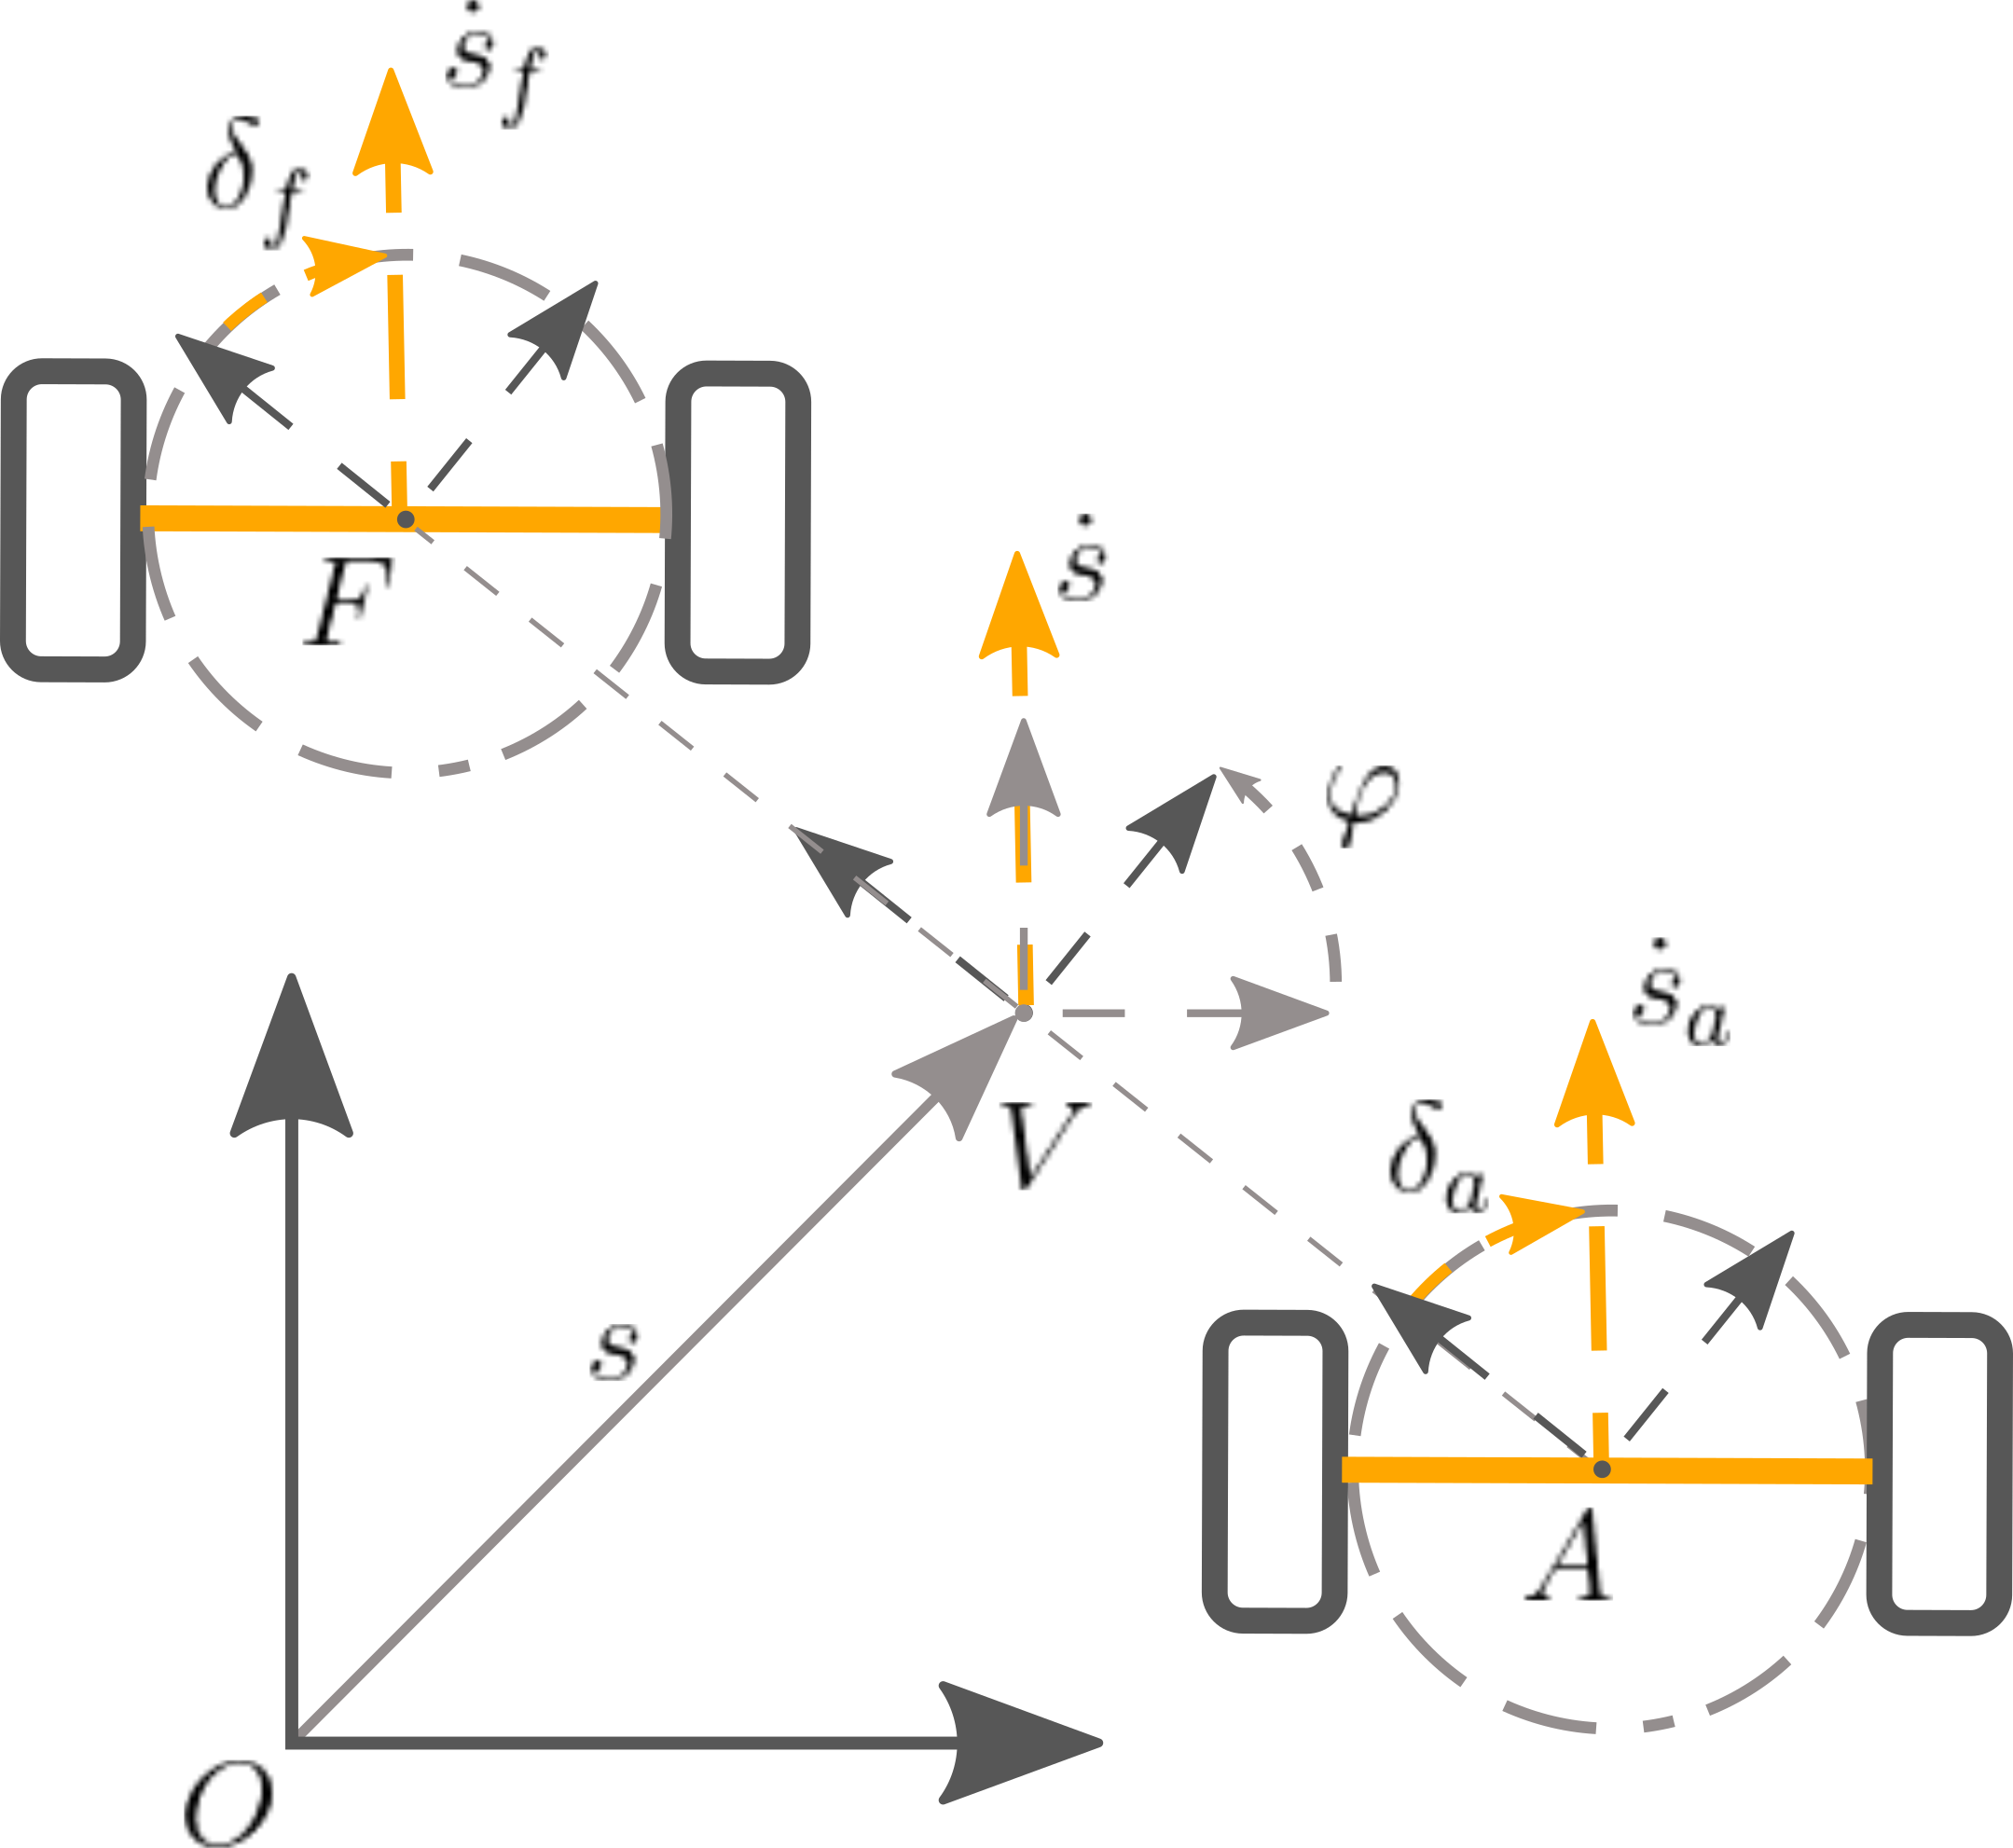
\includegraphics[width=0.6\textwidth]{figures/literature_survey/2Axle Vehicle Scheme.png}
    \caption{Two-axle vehicle system diagram. The vehicle main frame $V$ moves at velocity $\boldsymbol{\dot{s}}$, the front part $F$ at $\boldsymbol{\dot{s}_f}$ and the aft $A$ at $\boldsymbol{\dot{s}_a}$.}
    \label{fig:2Axle_Vehicle_Scheme}
\end{figure}

% Two axle vehicle requirements
The controller aims to control the vehicle sending torque signals to each of the wheels. For this, a reference generator will send the user's desired values for speed and steering, and a vehicle emulator will send the sensor values of the current displacement in each wheel. The controller must process these signals and convert them into torques. Further explanation on this subject is treated later in chapter \ref{sec:controller_in_TT_model}.\\

It is important to decide the frequency at which the controller is going to send new information to the actuators in the vehicle emulator. According to Aart-Jan de Graaf, company supervisor and main stakeholder regarding the vehicle control, the frequency control for propulsion is advised to be 10 samples per second, and for steering 20 samples per second. Because the controller does not discern speed from steering when sending the output signal, the control loop's frequency must be the fastest of the two, 20 samples per second. The feasibility of this is presented in chapter \ref{sec:Results} and discussed later in chapter \ref{sec:Discussion}.

\newpage

%%%%%%%%%%%%%%%%%%%%%%%%%%%%%%%%%%%%%%%%%
%% <<<<<<<<<<<<>>>>>>>>>><<<<<<<<<<<<< %%
%%%%%%%%%%%%%%%%%%%%%%%%%%%%%%%%%%%%%%%%%

\section{Literature survey} \label{sec:Literature_Survey}
This project system is compounded of several electronic boards that may run at the same time to send a consistent output to the vehicle actuators. This is a distributed vehicle controller that requires deterministic behaviour and synchronous communication.\\

%% Embedded distributed systems
% Cost reduction through standardization and safe increase with redundancy
There are many advantages when choosing a distributed control for a vehicle, such as optimization, robustness, simplified maintenance, standardization, economy or comprehensiveness, as presented in \citep{advantages_distributed_control}. This thesis focuses on the robustness aspects of the controller. There are different strategies to ensure robustness in a system such as fault containment units and triple modular redundancy \citep{kopetz_robustness}, along with Time-Triggered communication \citep{kopetz_tt_comm}. The main controller is deployed onto three independent boards that can reset when a fault is detected. These boards make the same calculations to make sure the output value is correct even if one of the boards has failed. These mentioned strategies together with double channel communication are employed in this project to make the system fully-redundant.\\
% Fault Containment Units
% Triple modular redundancy
% Distributed vehicle controllers

%%%%%%%%%%%%%%%%%%%%%%%%%%%%%%%%%%%%%%%%%
%% Vehicle controllers
Vehicle controllers are usually decoupled into a velocity (longitudinal) controller and a steering (lateral) controller, as it can be seen in the proposals from \citep{control_strategies_auto_vehicles} and \citep{tech_review_control_aut_ground_vehicles}. These articles also pay special attention to the vehicle physical limitations and define the output limits of the actuators. The controller presented in this thesis is also internally divided into steering and speed but the physical analysis is different from common vehicles, as the control is performed over a two-axle vehicle. The input and output ranges and units are already defined by design. The controller cycle frequency for autonomous vehicles is usually recommended to be 100$\,$Hz, as can be seen in \citep{controller_arch_autonomous_vehicle}, but Aart-Jan de Graaf, the company supervisor of this thesis, has personally recommended that 20$\,$Hz is enough for this project's application.\\
% Autonomous vehicle controllers

% Distributed controller
% Communication channels in vehicle distributed applications
An example of a distributed controller for an autonomous ground vehicle can be found in \citep{distributed_all_terrain_vehicle}. The vehicle tasks in this article are very complex, as it is an all-terrain vehicle and requires communication among different sensors and processors. Communication is held via CAN-network. When looking at other automotive protocols for communication, \citep{automotive_comm_protocols} presents other choices apart from CAN, such as Local Interconnect Network, FlexRay or media-oriented system transport.\\
% Different communication channels in automotive systems. The STM32 E407 and HANcoder are compatible with CAN.


%%%%%%%%%%%%%%%%%%%%%%%%%%%%%%%%%%%%%%%%%
%% Time Triggered communication design
% TTCAN
% Some ideas about TTCAN paper, and differences with our approach because of HANcoder limitations
The system of this thesis uses Time-Triggered communication over CAN, which is very similar to the Time-Triggered CAN (TTCAN) protocol presented in \citep{ttcan}. The communication protocol employed using HANcoder cannot follow all the specifications of TTCAN, as later explained in chapter \ref{sec:method_master_slave_strategy}. The main feature both protocols have in common is that they set an extra layer over CAN with a Time-Triggered offline schedule.\\

% Task model
% Task model from one of the papers, with Tx messages and Rx messages, one after another to exchange information between nodes.
To find an appropriate schedule it is important to define how the communication tasks are going to be handled in the system. The model employed in this project is based upon some ideas proposed by \citep{comp_comm_task_model}. It defines a phase parameter $\phi$ to decouple the computation from the communication of a task. This project uses this parameter as a delay to separate when the communication task starts and when the message is actually sent. More information about the task model is discussed later in chapter \ref{sec:tt_comm_model}.\\

\newpage

% schedule for mixed computation - communication applications
The Time-Triggered schedule for this project requires taking into account the computational and communicational aspects of the tasks. The article by \citep{optimal_comm_schedule} dives into the mathematical analysis of a schedule with computational tasks that depend on the network message transmission, either receiving messages, transmitting them or both. It also proposes an optimal scheduling strategy considering the message-computation relationships and tries to find a solution with a minimum matrix period cycle.\\

The schedule of the project is simple enough not to require an algorithm to set it but it takes ideas from \citep{optimal_comm_schedule} to set the correct order of tasks and dependencies among calculations and messages. This article also discusses the challenges they encountered when deploying a real-time system, such as the increase in the time of the computational tasks due to the overhead in the deployed Free Real-Time Operating System (FreeRTOS). Even though they calculated the Worst-Case Execution Time (WCET) with analytical techniques, the resulting measured time of the tasks period when the system was deployed was higher. The system for this thesis is also deployed over a FreeRTOS and, as described in \citep{optimal_comm_schedule}, making analytical calculations of the WCET is very hard. As proposed in \citep{wcet}, the execution time of the tasks will be measured and a 20$\%$ safety margin will be added to the result to estimate the WCET of each task in the matrix cycle.\\
%% Challenges in deployment
% measuring ET as an approach to WCET

% RealTime communication using MATLAB
There is also work made around the creation of real-time schedules for distributed embedded applications using \textsc{Matlab}. As described in \citep{RTW_matlab} and \citep{TT_task_schedule_matlab}, there are specialized toolboxes to work with schedules and resource sharing. However, this project focuses on the development of the software just using basic Simulink and HANcoder blocks.\\

%%%%%%%%%%%%%%%%%%%%%%%%%%%%%%%%%%%%%%%%%


%%%%%%%%%%%%%%%%%%%%%%%%%%%%%%%%%%%%%%%%%
%% <<<<<<<<<<<<>>>>>>>>>><<<<<<<<<<<<< %%
%%%%%%%%%%%%%%%%%%%%%%%%%%%%%%%%%%%%%%%%%

\newpage
\section{Methodology} \label{sec:methodology}
% Overview
The objective of this project is to deploy a distributed controller with Time-Triggered communication for the two-axle vehicle described in \citep{two_axle_vehicle}. In order to achieve this the project development is divided into different phases that shape the parts of the system:
\begin{enumerate}
    \item Time-synchronous system.
    \item Time-Triggered controller.
    \item System deployment and testing.
\end{enumerate}

These phases are presented and explored in this section. The different reasoning behind each development choice, deployment procedure and the testing option is explained in each subsection. As an initial overview, a scheme of the whole system and its components is shown in figure (\ref{fig:system_overview}). This scheme shows, from top to bottom, the software, hardware and monitor components, respectively.\\

\begin{figure}[h!]
    \centering
    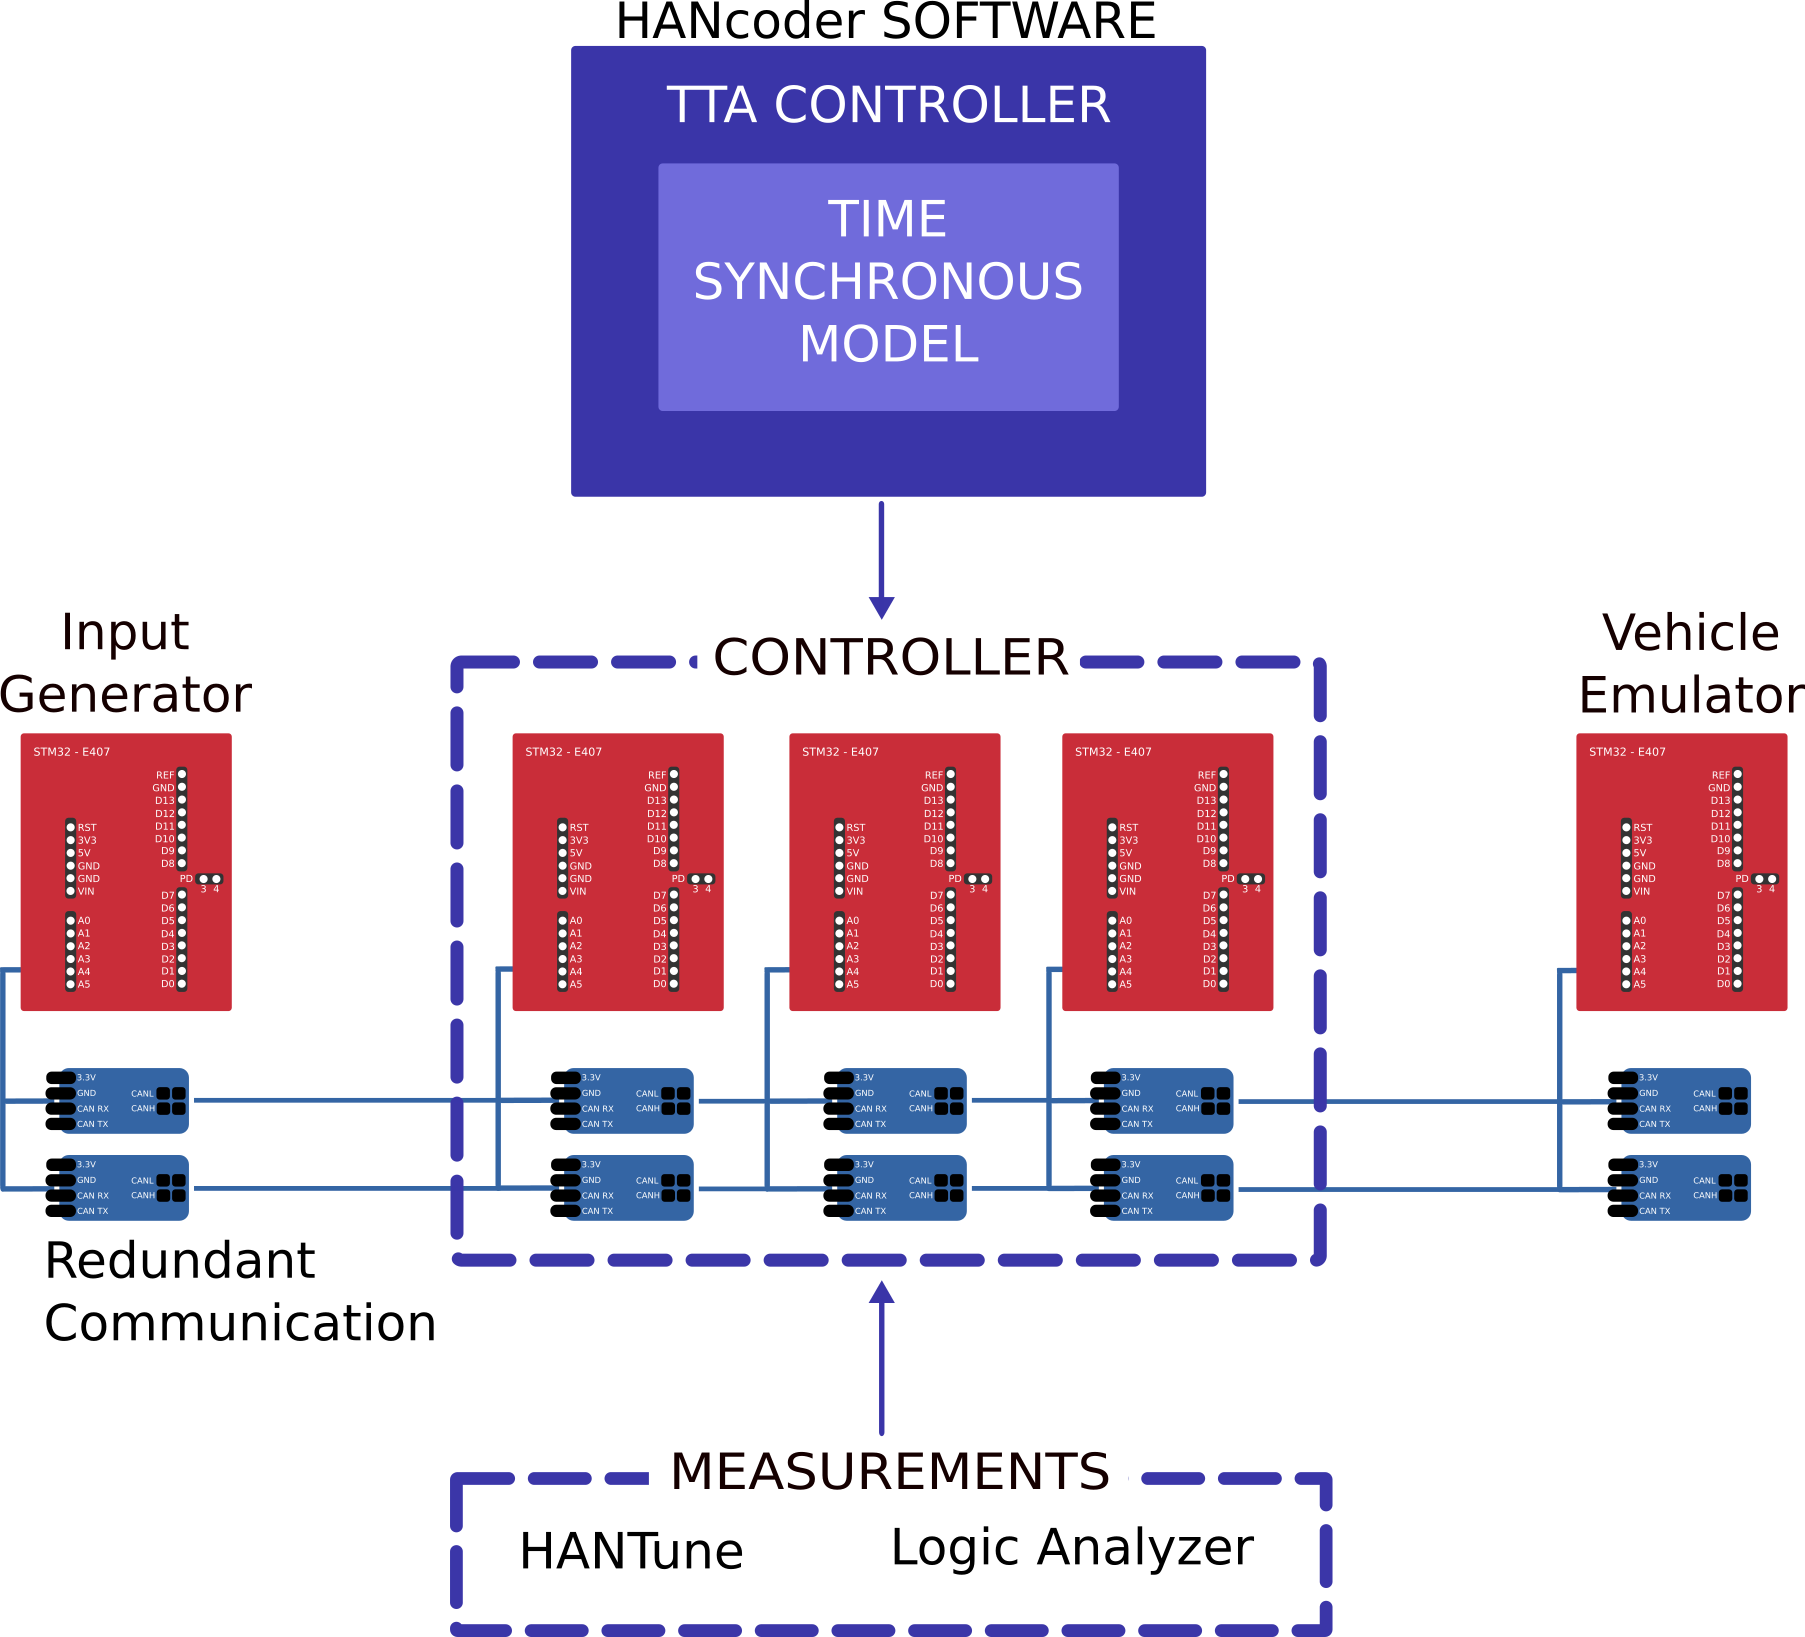
\includegraphics[width=0.8\textwidth]{figures/methodology/methodology_lowres.png}
    \caption{Overview of the whole system. The red components are STM32-E407 boards that contain the system's software. The blue components are CAN transceivers that set a double CAN communication network and allow the boards to communicate with each other.}
    \label{fig:system_overview}
\end{figure}

The system software is divided into the time-synchronous model, which is in charge of keeping the controller boards synchronized, and the Time-Triggered Architecture (TTA) controller software, which processes the inputs from the two-axis vehicle and converts them into the signals output to the vehicle emulator. The hardware components consist of five boards, one for the input generator, three for the controller and one for the vehicle emulator, and ten CAN transceivers, for double CAN communication. There are three controller boards to have triple modular redundancy on the controller decisions and double CAN communication to have redundancy on the message exchange between the boards. The monitor components employed in this project are HANTune, with which it is possible to see the software signals in real-time, and a logic analyzer with eight channels, which allows for monitoring digital signals on the boards. HANTune is very helpful to see how the software signals change while the code is running, but its sample time is limited to $100\,$Hz and it increases the system overhead. The logic analyzer is used when it is necessary to check the behaviour of the system at a task activation level.\\

Before diving into the different project phases, it is important to declare a set of hardware and software features that determine the boundaries of the possible performance of the current version of the prototype. After these limitations are presented, an overview of the core ideas behind the Time-Triggered schedule is described. With these ideas in mind, the synchronization basic cycle, the controller basic cycle and the input generator and vehicle emulator matrix cycles are explained in order. A brief overview of the software architecture is then assessed and finally, the methodology is finished with a description of the system deployment and testing strategies.

%%%%%%%%%%%%%%%%%%%%%%%%%%%%%%%%%%%%%%%%%
% Limitations
\subsection{Limitations}
The main hardware choice is the STM32-E407 board, as it is the only board supported by HANcoder to use CAN communication with two CAN channels. Both the hardware and software choices by the client impose some limitations on the project. For instance, HANcoder and HANTune are the sources of the following ones:
\begin{enumerate}
    \item HANcoder deploys FreeRTOS with its software. The operations of this Operating System (OS) create a big overhead on the processor when the hardware Interrupts ReQuests (IRQs) of the software are too frequent. It has been observed that the conflicts between OS and IRQs happen with $100\,$kHz granularity on the interrupts.
    \item HANTune requires connecting the development computer with the board to monitor the software signals. These connections employ some of the FreeRTOS resources for communication, so using HANTune while the IRQs are frequent increases the overhead even more.
    \item Software development with HANcoder is limited by the blocks offered by the program. One could develop more blocks by coding with \textsc{Matlab} or C, but the client suggests avoiding this when possible to prioritize software model development. The software proposed is based on the creation of new functionalities by using the current blocks, but some high-level blocks allow for little extra configuration, such as the blocks regarding CAN communication.
    \item The software governing the two CAN channels in HANcoder does not allow them to be independent, so redundancy using these two channels does not improve the robustness of the system. This is because both channels share a buffer at a low C programming level, thus if one of them fails, the other stops working too. This is ignored during the rest of the project as the client has already contacted the HANcoder development team to correct this problem. It is expected that newer versions of HANcoder will allow for using both CAN channels for robustness, but it is not clear when this will happen. A prototype has been developed for this project soldering all the CAN communication connections to reduce the chances that a communication problem arises because of loose cables.
\end{enumerate}

The main hardware limitation is imposed by the STM32 boards. The number of connections of the board limits the number of elements that can be connected to them. At the moment the required connections are four pins for communication and three pins for unique board identification. This hardware limitation does not have a heavy impact on the project. This is because there are enough connections in the boards for the required functionalities. However, this may change in case this project had to be extended in the future.\\

%%%%%%%%%%%%%%%%%%%%%%%%%%%%%%%%%%%%%%%%%
% TT schedule overview
\subsection{Time-Triggered schedule overview}

%% Explain the relations between Time-Triggered communication, basic and matrix cycles, Time Marks, clock granularity, frequency of the IRQs vs frequency of the controller and the concept of task.
A Time-Triggered schedule is compounded of different tasks, either for computation or communication, that must happen in predefined time windows (TW). The moment in time when each TW starts is called time mark and they are numbered along a basic cycle. The project has a task schedule (or matrix cycle) that counts with two basic cycles, the first for time synchronization and role selection (presented in subsection \ref{sec:method_master_slave_strategy}) and the second for the controller calculations (presented later in subsection \ref{sec:controller_in_TT_model}). An example of a standard matrix cycle is presented in figure \ref{fig:matrix_cycle_example}. 

% matrix cycle example
\begin{figure}[h!]
    \centering
    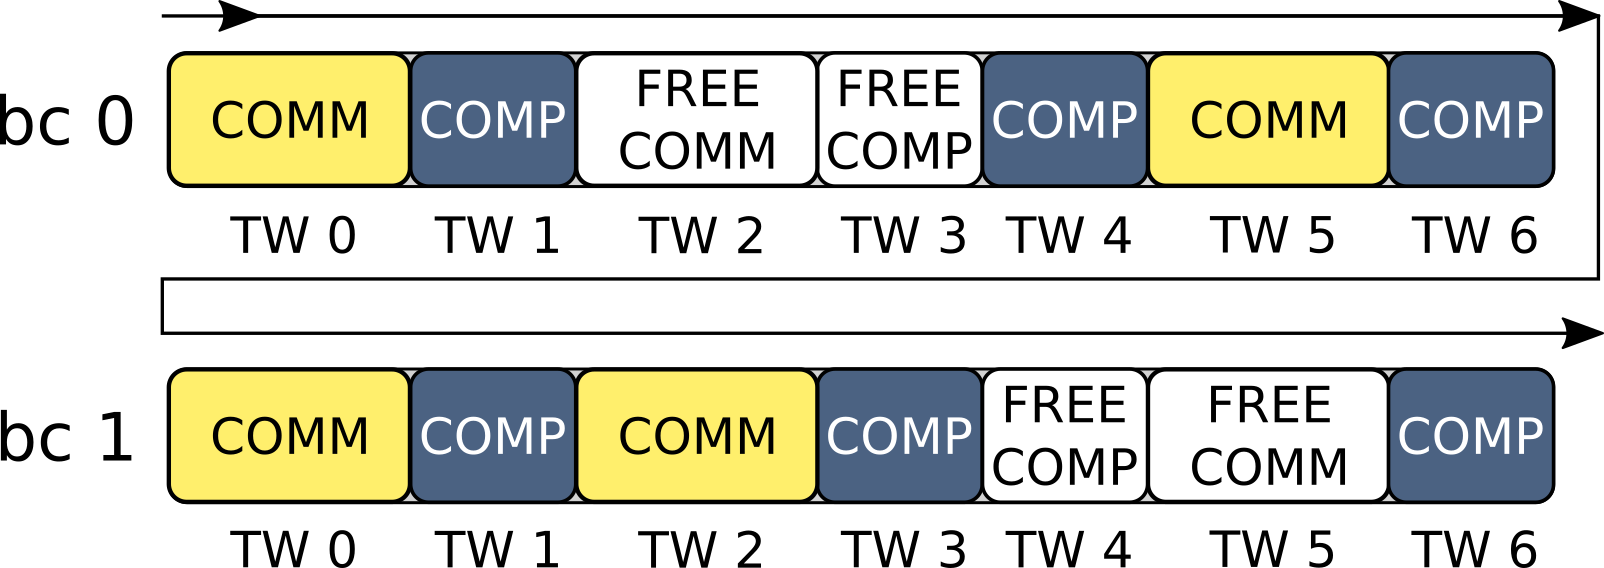
\includegraphics[width=0.8\textwidth]{figures/methodology/matrix_cycle_example.png}
    \caption{Matrix cycle example. It is compounded of two basic cycles (bc0 and bc1) with a series of time windows (TW). The different tasks presented are either communication tasks (COMM) or computational tasks (COMP).}
    \label{fig:matrix_cycle_example}
\end{figure}

%% Introduce matrix cycle example and explain basic elements
The matrix cycle example from figure (\ref{fig:matrix_cycle_example}) is read from left to right and from top to bottom, as the arrow path shows. There are two different kinds of tasks: communication and computation tasks. During a communication task, one of the boards transmits a message and the others wait for the message to be received. Every message is transmitted several times during the same communication task with the same information, to raise the chances the message reaches its destination. In this project proposal, every communication task is followed by a computational task that processes the contents of the message (if any was received). A computational task handles any kind of operation that does not involve communication. There can be free time windows, where there is no task scheduled for that period.\\

The basic cycles of a matrix cycle usually have the same length (in time). This is because the length of a basic cycle is in most cases determined by the time required to synchronize the boards again. Because each board has its own local time governed by its own clock, the frequency of the clocks of the different boards does not have to be exactly the same. This can cause a drift between the boards. This is why the boards are not synchronized just once, but regularly, at the beginning of every basic cycle with what is called the reference message. This reference (or sync.) message contains the global time information from the time master board to ensure all boards remain synchronous. This project does not follow the idea that both basic cycles shall have the same period though. The limitations found in communication and computational time (presented later in section \ref{sec:Results}. Results) combined with the recommendation of making the complete matrix cycle duration 20 Hz do not leave much free time to spare in free windows during the controller matrix cycle. The drift of the boards is not as important as to desynchronize them before each reference message so it was preferred to divide the matrix cycle regarding task objectives instead of precision time for scalability and system comprehension.\\


%%%%%%%%%%%%%%%%%%%%%%%%%%%%%%%%%%%%%%%%%
\subsection{Time synchronous model}\label{sec:time_sync_model}
We need the system boards to be able to send and receive messages independently at some precise moments in time. This requires them to share a consistent global time. The global time is set by one of the controller boards, the master, and followed by the other boards in the ensemble, the slaves. The basic cycle that ensures there is an agreed master is presented in section \ref{sec:method_bc0}. It is essential that in case the master fails one of the slaves takes its place as master so the system does not stop working synchronously. The reasons behind choosing the plan followed in section \ref{sec:method_bc0} are discussed in the Master-Slave decision strategy subsection \ref{sec:method_master_slave_strategy}. The boards must be properly synchronized for the whole schedule to work, so their basic cycles happen at the same time. Every message sent and received by each node is planned to happen within the same framework, called the communication task model. This model is presented in the Time-Triggered communication task model in subsection \ref{sec:tt_comm_model}.

%%%%%%%%%%%%%%%%%%%%%%%%%%%%%%%%%%
\subsubsection{Synchronization basic cycle}\label{sec:method_bc0}
% Controller in charge of global time. Reference generator and vehicle emulator just follow the master's time.
When the system boards are turned on they wait to receive a reference message from a master that has awakened before them. If a board from the controller does not receive any reference message during a matrix cycle time, it will proclaim itself as the master of the ensemble and will start the first basic cycle. Hopefully, some other board will have already been listening by this moment and they will synchronize. From that moment on the system will execute the tasks from the matrix cycle in order. In case the time master of the ensemble fails to share the reference message, one of the other boards should take the master role instead. The strategy followed to ensure that there is a time master board sharing a correct time reference at the beginning of the controller calculations is based upon an election held among the three controller boards. This poll is performed during a whole basic cycle, as represented in figure (\ref{fig:master_election_basic_cycle}).\\

%% include master election basic cycle scheme!!
\begin{figure}[h!]
    \centering
    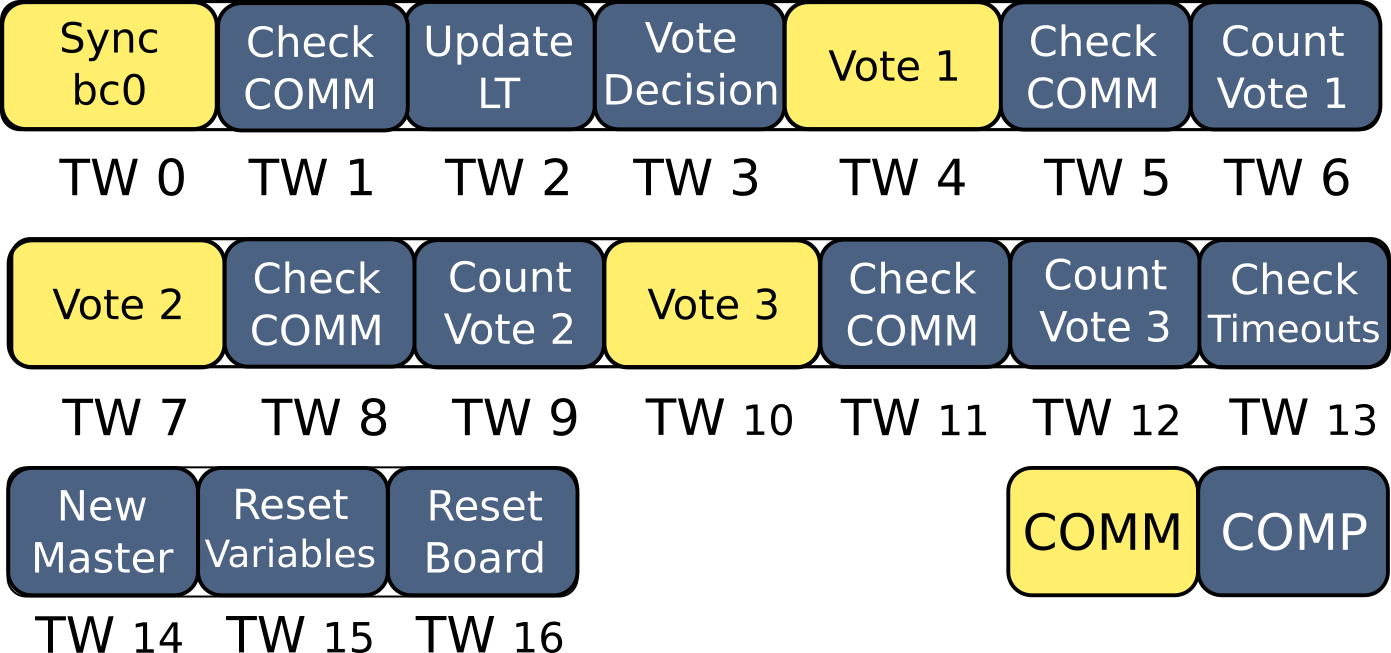
\includegraphics[width=0.8\textwidth]{figures/methodology/basic_cycle_election.png}
    \caption{Basic cycle scheme for the election process when choosing a time master. Communication (COMM) tasks are painted in yellow and computational (COMP) tasks are painted in blue.}
    \label{fig:master_election_basic_cycle}
\end{figure}

The first task activating at the beginning of the basic cycle is the communication task \textit{Sync bc0} for board synchronization. During this communication task, the master shares its local time with the so-called reference message, thus the slaves can synchronize with it.
Every communication task is followed by a computational task, \textit{Check \textsc{comm}}, to analyze the messages received by both CAN channels (if any). In case any message has been received, or none of the messages received is considered coherent, a failure will be acknowledged and the message will be considered as missed. If both messages are received and are coherent, the message from CAN channel 1 is processed.\\

The slaves update their own local time during the \textit{Update LT} computational task. The local time update takes into account the difference between when the reference message is expected to be received and when it is actually received. This difference is called the desynchronization of the board. If the desynchronization is negative the local time is reduced and none of the already performed tasks is repeated. If the desynchronization is positive the local time is increased in small steps to ensure that no task is skipped. However, if the reference message is either regarded as incorrect or has not been received at all, the slave board considers the master at fault and decides to vote for another board to be the new master. The vote decision happens during the \textit{Vote decision} computational task. When the time reference is received and it is consistent with the local time, then the vote is cast for the current master. Otherwise, the board with the lowest error count apart from the current time master is chosen. The error counter increases for each board every time a message from that board is not received. The criteria on how to choose which board to vote are depicted in a flow chart in appendix \ref{app:vote_criteria}.\\

The communication tasks that are used to exchange the voting information are \textit{Vote 1}, for the vote of board 1, \textit{Vote 2}, for the vote of board 2 and \textit{Vote 3} for the vote of board 3. The board transmitting the board information (for example, board 1 during \textit{Vote 1}) broadcasts to the other boards the board ID of the board that it believes should be the master board for this matrix cycle. The boards receiving information activate the corresponding \textit{Count Vote} computational task to take that vote into account for the election.\\

In the \textit{Check Timeouts} computational task it is considered which messages were not received during the basic cycle so the error counter for the board whose message was not received is increased by one (fault detection). If no messages have been received by a board during this basic cycle a flag is set to reset the board at the end of the basic cycle. In the \textit{New Master} computational task the master is decided regarding the votes received from the election. During the \textit{Reset Variables} task different variables are reset to make the board ready for the next basic cycle. If the reset flag is set, in the \textit{Reset Board} computational task the variables in charge of initialization are reset so the board returns to a state in which no role is still assigned and waits until a reference message is received.\\


%%%%%%%%%%%%%%%%%%%%%%%%%%%%
\subsubsection{Master - Slave decision strategy}\label{sec:method_master_slave_strategy}

The TTCAN document \citep{ttcan} presents a different simpler strategy to choose a new master when the current master fails. This procedure assumes every message sent to the CAN network is broadcast and has a certain priority. However, HANcoder CAN blocks cannot fulfil these two requirements at the same time.\\

A message can be sent with a specific ID, which sets the message priority, but another board that wants to receive this message has to check for messages with that specific ID in the network. This means that messages are not effectively broadcast. For the broadcast to be effective, every time a message is sent an interrupt should happen in the receiver end of all other boards. It is also important that checking if a message has arrived happens as soon as possible after the message has actually arrived, as otherwise the board receiving the message cannot compare its own time with the reference time received.\\

It could also be possible to send all messages with the same ID so the boards do not have to pay attention to different IDs, but this would mean that all messages have the same priority, so the strategy from \citep{ttcan} could not be performed either. The strategy proposed in this project is complex and time-consuming, but it ensures that in case of time master failure one of the other boards will take its place in a democratic and organized manner. It is also important to remark that for the message exchange to work every board must be synchronized, otherwise, they could miss the message received. The moment a board does not receive messages from any other board, it performs an auto-reset (\textit{Reset Board} computational task), so it can synchronize again with the next reference message.


%%%%%%%%%%%%%%%%%%%%%%%%%%%%%%%%%%%
\subsubsection{Time-Triggered communication task model}\label{sec:tt_comm_model}
Every communication task in the program is defined by the same model, either if the board executing the task is transmitting or receiving. A board that should transmit a message during a communication task will wait until the appropriate moment to send it. If more than one message is programmed to be sent during the same task, these are sent in the appropriate moments through the correct channels. A board that is supposed to receive a message during the communication task will ask the CAN interface at every IRQ to check if a new message has arrived.\\

A communication task has a time limit $\uptau$ since the moment it starts, called period. The message is sent after a known time $\phi$ since the task starts, called phase. The time $\delta$ between transmission and reception is the communication delay. If the board is transmitting it sends the message through the CAN send block $\phi$ ticks after the task starts. If the board is listening it checks the CAN receive block every cycle from start until the message is received or a maximum time of $\uptau$ ticks passes. If the message is not received at this time, it is considered lost and the matrix cycle keeps going on. If the message received is the master's reference time, analysis on when the message was received is held to make any changes on the current local time if necessary. This requires the communication delay to be known, a value presented later in section \ref{sec:Results}. Results. An example of how the communication is held with three boards with just one message being sent through one channel is presented in figure (\ref{fig:com_task_ex}).\\

% include communication task model example scheme!!
\begin{figure}[h!]
    \centering
    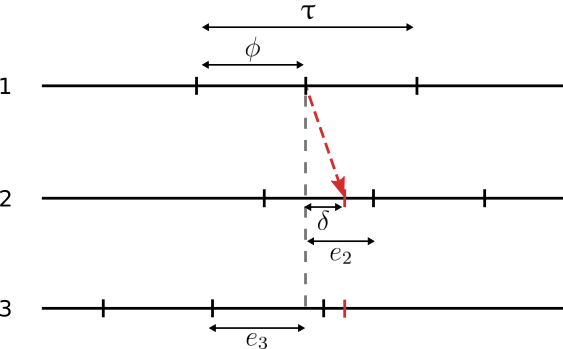
\includegraphics[width=0.7\textwidth]{figures/methodology/comm_task_ex.png}
    \caption{Communication task example between three nodes.}
    \label{fig:com_task_ex}
\end{figure}

In the example from figure (\ref{fig:com_task_ex}), board number (1) works as the master while boards (2) and (3) are slaves. Boards (1) and (2) are synchronized well enough (time error $e_2$ is smaller than $\phi + \delta$). This means board (2) receives the message and acknowledges the time error $e_2$, so it can correct it for the next cycle. Board (3) is not synchronized enough with board (1) (time error $e_3$ is bigger than $\phi - \delta$), so it misses the message. If board (3) does not receive any other message from the ensemble it will auto-reset at the end of the cycle. If it does receive messages from board (2) because it is better synchronized with it, board (2) will receive more votes in the next election, it will become the new master and all other boards will synchronize with it.\\

The example from figure (\ref{fig:com_task_ex}) shows just one message being sent from board (1) to the others. With two CAN communication channels, this corresponds to the scenario when messages from both channels have the same phase ($\phi_1 = \phi_2$). However, in this project, these phases $\phi_1$ and $\phi_2$ are not the same, as this way the messages are more likely to be received by other boards. The longest the time between $\phi_1$ and $\phi_2$, the broader the time band in which the messages can be received by other boards. Moreover, more than one message is sent through each channel during a communication task, to increase the chances of reception even more. The maximum amount of messages that can be sent through a channel has been set to seven. This is because only the first byte of every message sent has been allocated to temporal information. This temporal information includes (1) the ID of the sender with 4 bits, (2) the basic cycle in which the message was sent with 1 bit and (3) the message count of the transmitted message with the 3 remaining bits. The other seven bytes in every message contain each an unsigned eight (uint8) data value. If the value that is transmitted was originally a float variable it has to be coded into an uint8 data value before the transmission and decoded back to float at the receiving end. The coding strategy chosen is explained in appendix \ref{app:float2uint8}.\\

When communication is held, because of how the CAN blocks in HANcoder work, the receiving board should be waiting for the message in advance with the message buffer clean in order to receive both the value and the time when the appropriate message arrives. A state machine in three stages has been developed to get the correct message in time. (1) First the CAN receive block is called to empty the message buffer. (2) Then the block is called repeatedly until a message arrives. (3) The message content is forwarded to the communication check task.

%%%%%%%%%%%%%%%%%%%%%%%%%%%%%%%%%%%%%%%%%
\subsection{The controller in the Time-Triggered model} \label{sec:controller_in_TT_model}
The distributed controller employed for this project is based upon a basic PID CAN distributed controller designed by \citep{former_model}, in which both supervisors of this Master thesis contributed. This controller is internally divided into steering and speed controllers, using some basic calculations to convert the user set points and the sensor signals into the actuator signals for each wheel. A scheme representing the message exchange with the variable values among the reference generator, controller and vehicle emulator is presented in figure (\ref{fig:controller_signals}). Detailed information about the controller operations is presented in appendix \ref{app:controller_operations}.\\

%% include scheme of the reference generator - controller - vehicle emulator, signals!
\begin{figure}[h!]
    \centering
    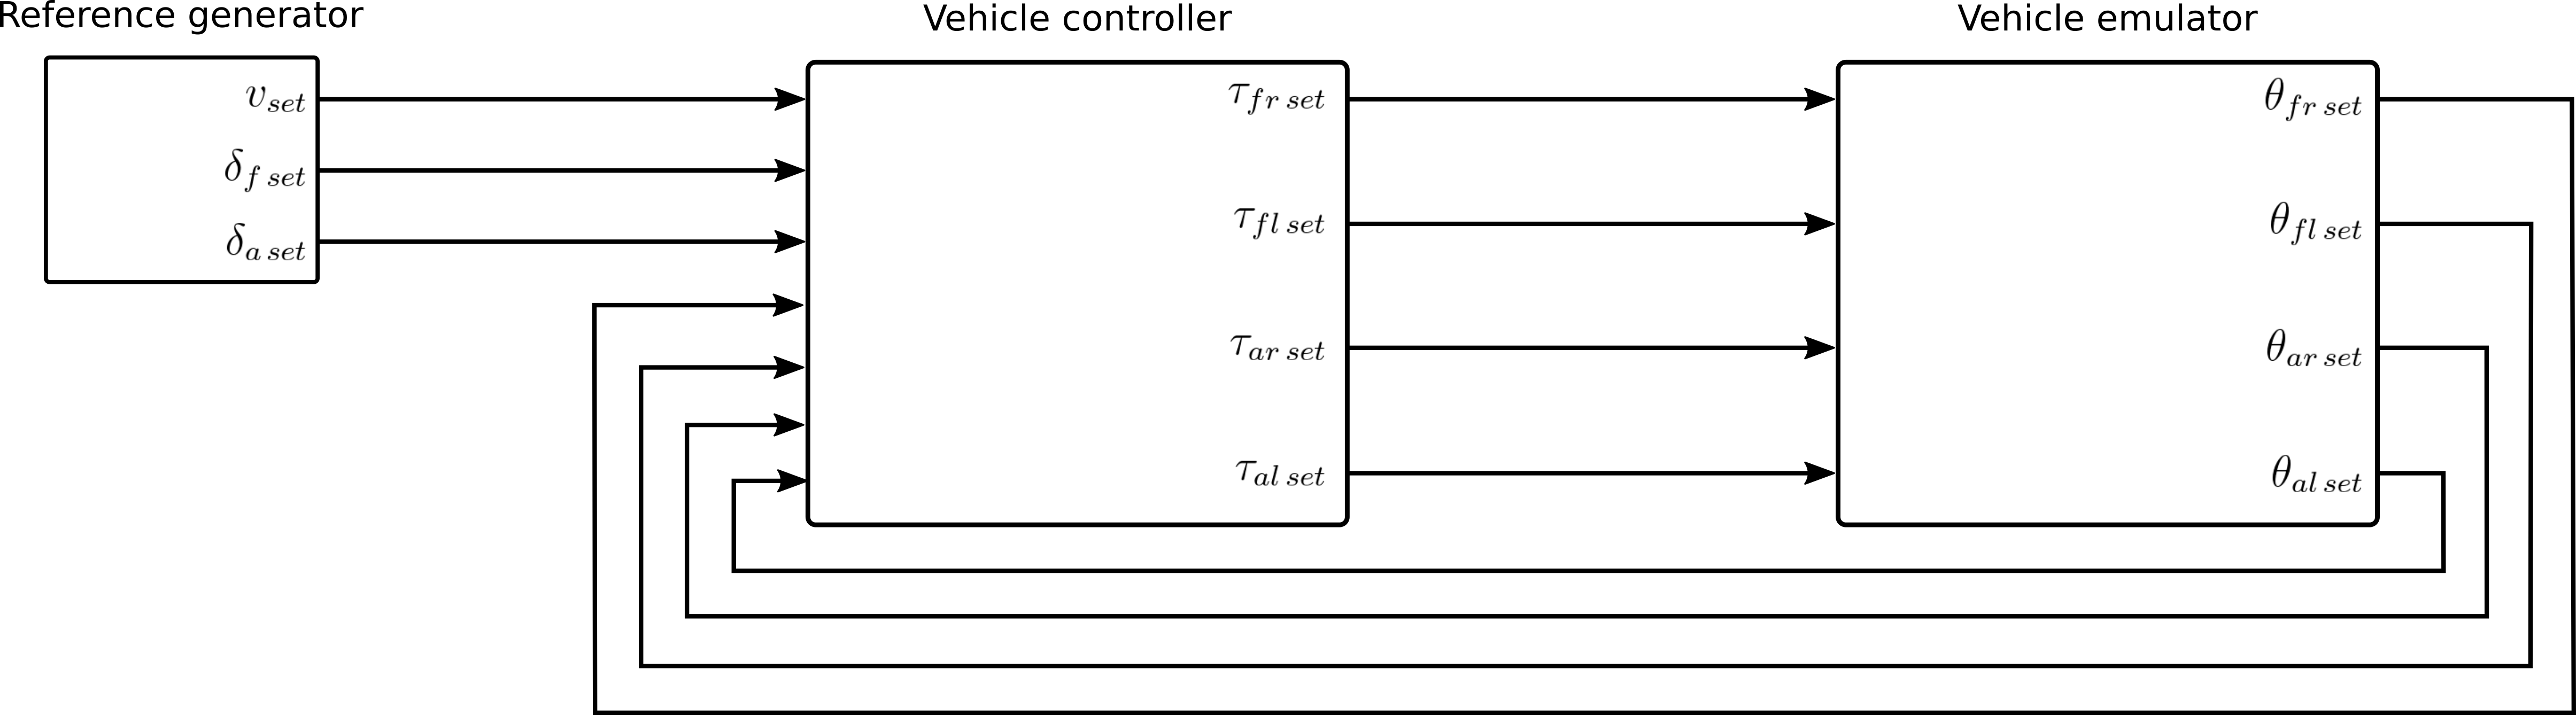
\includegraphics[width=\textwidth]{figures/methodology/signals_scheme.png}
    \caption{Signal exchange between reference generator, vehicle controller and vehicle emulator. The reference generator sends the set velocity $v_{set}$ and the steering angles for the front $\delta_{f\,set}$ and for the aft $\delta_{a\,set}$. The vehicle controller receives the signals from the reference generator and the sensor values from the vehicle emulator, which correspond to the displacement $\theta_{set}$ on each of the wheels. The vehicle controller also outputs the torques $\tau_{set}$ of each of the wheels to the vehicle emulator.}
    \label{fig:controller_signals}
\end{figure}


The controller operations basic cycle can be found in figure (\ref{fig:controller_basic_cycle}).

%% include controller basic cycle scheme!
\begin{figure}[h!]
    \centering
    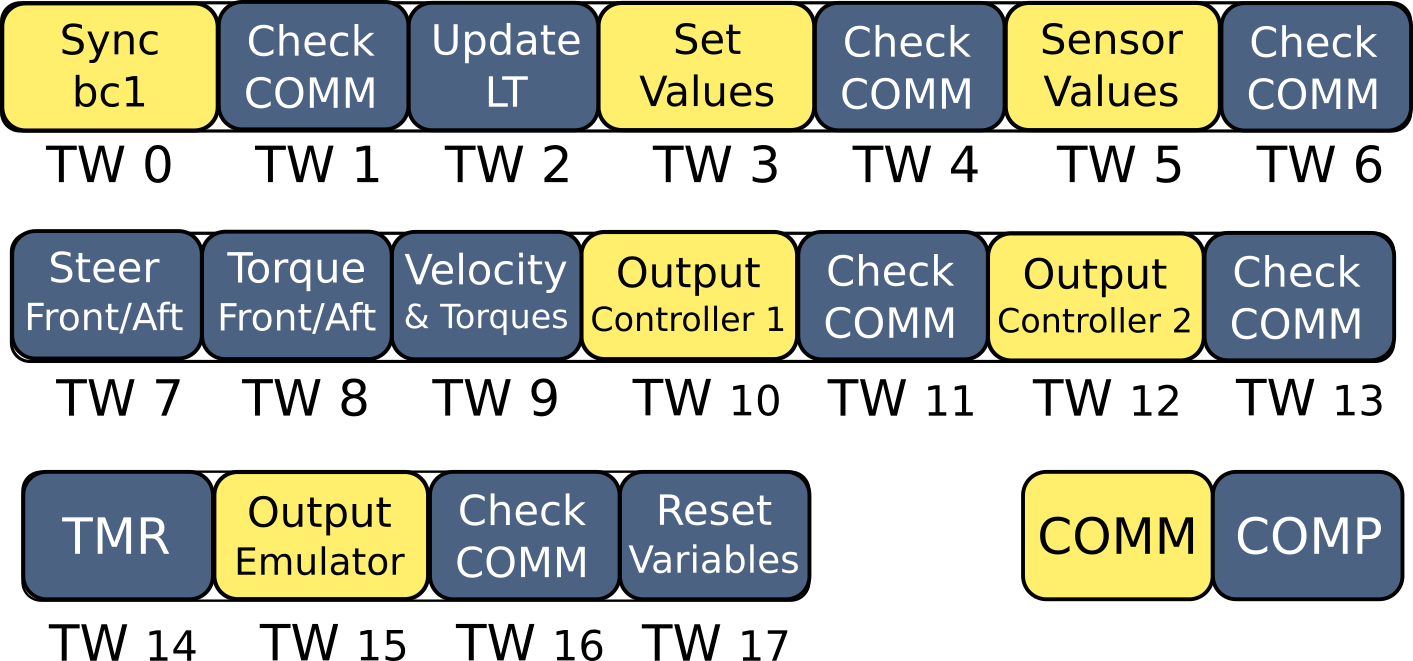
\includegraphics[width=0.8\textwidth]{figures/methodology/basic_cycle_controller.png}
    \caption{Basic cycle for the controller operations. Communication (COMM) tasks are painted in yellow and computational (COMP) tasks are painted in blue.}
    \label{fig:controller_basic_cycle}
\end{figure}

The beginning of the controller basic cycle is identical to the time synchronization basic cycle. The master board sends the reference message with the global time and the slave boards update their own local time depending on the desynchronization. The next two communication tasks are the \textit{Set values}, to receive the information from the input generator, and the \textit{Sensor values}, with the information of the vehicle emulator.\\

From then on, the different operations to calculate the output signal are performed in consecutive tasks. These calculations are performed by all the controller boards, presumably getting (almost) identical results. When the calculations are done, the slave boards broadcast their output values with the communication tasks \textit{Output Controller 1} and \textit{Output Controller 2}. These values are received and checked by the master board, so it can perform the Triple Modular Redundancy operation (\textit{TMR} computational task). If at least two of the values are consistent with each other, the master will output the one received first at the \textit{Output Emulator} communication task. In case there were several faults in the calculation of the next output value for the vehicle emulator, the master board outputs an empty message. Apart from the output information for the vehicle actuators, the controller also sends information about the communication and TMR errors with an error log.\\

The complete system controller matrix cycle is compounded by the two already presented basic cycles: the master election from figure (\ref{fig:master_election_basic_cycle}) and the controller operations from figure (\ref{fig:controller_basic_cycle}). At the beginning of each basic cycle, the global time is shared by the master to remove the time drift from the other boards. These basic cycles are executed one after the other in succession from the moment the initialization finishes while the system is operating. A representation of how both cycles look together is presented in figure (\ref{fig:matrix_cycle}).\\

%% include matrix cycle scheme!
\begin{figure}[h!]
    \centering
    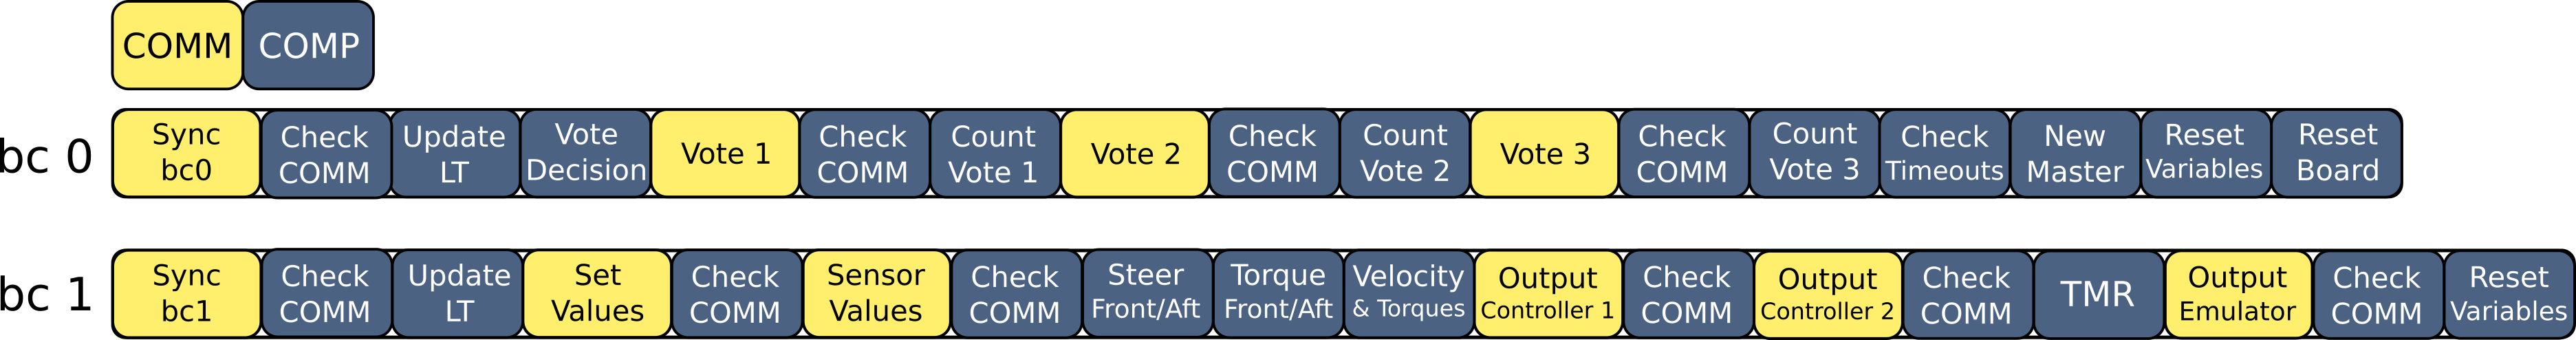
\includegraphics[width=\textwidth]{figures/methodology/matrix_cycle_controller.png}
    \caption{Matrix cycle of the vehicle controller. Communication (COMM) tasks are painted in yellow and computational (COMP) tasks are painted in blue.}
    \label{fig:matrix_cycle}
\end{figure}

Regarding software merging of the Time-Triggered controller into the time synchronous model, information on how the different basic cycles are managed can be found in section \ref{sec:software_overview}.\\

There is some common information required at the controller calculations for all the controller boards to get results as close as possible to each other: the integral sums. If a board stops its operation for some time and then gets auto-reset (or even hard-reset) it requires information from the current integral state of the system. The idea of the ground state is introduced to solve this problem, so with every reference message, along with temporal information, value domain information with the integral calculations are shared from the master to the other boards. This way, a freshly synchronized board will have the right information to make the same operations as the other boards in the ensemble so the TMR operation regards those calculations as valid too. The current prototype proposal does not require much ground state information to be shared at every reference message, so a single reference message suffices to share all the required data.


%%%%%%%%%%%%%%%%%%%%%%%%%%%%%%%%%%%%%%%%%
\subsection{The input generator and vehicle emulator}\label{sec:inputgen_vehicleem}
Both input generator and vehicle emulator were already designed in a Simulink model structured to follow Simulink time instead of hardware interrupts. For this project, it is important to redesign both so the communication between them and the controller remains synchronous. Their operations were divided into tasks like it was done for the controller. However, they must do fewer calculations over the matrix cycle process, as they are not in charge of the time master decision and have less communication exchange with the ensemble. They synchronize their own local time every time they receive the reference signal, regardless of which board sent the message and reset after doing their calculations if no reference message was received. It is important for them to expect the reference message at a specific time window so they are required to follow a similar matrix cycle structure. Resetting as soon as possible when no reference signal has been received is important to focus on resynchronization.\\

% Input generator creates signal values according to HANTune. These signals are sent to the controller at the third time window of the controller operations basic cycle.
The input generator uses the set signal values defined at HANTune. These signals are sent to the controller in the \textit{Set Values} communication task of the controller operations basic cycle, as it can be seen in figure (\ref{fig:controller_basic_cycle}). The input generator matrix cycle is presented in figure (\ref{fig:input_generator_basic_cycle}).\\

\begin{figure}[h!]
    \centering
    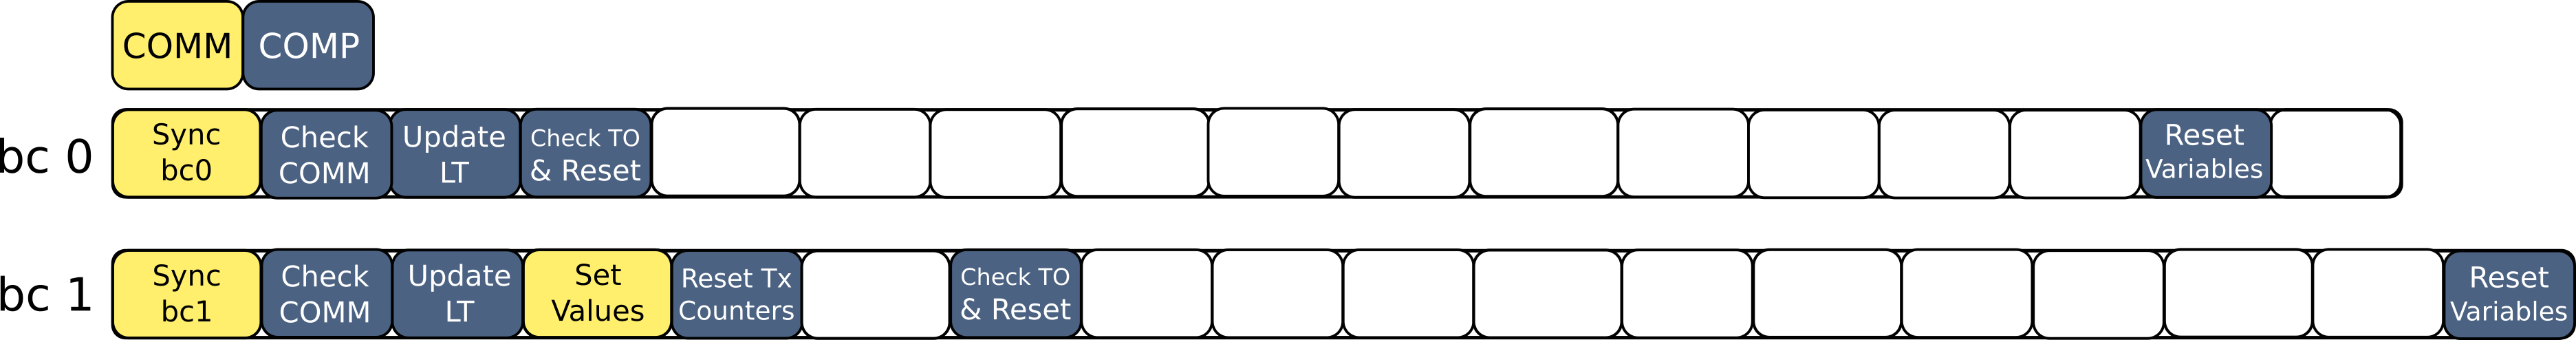
\includegraphics[width=\textwidth]{figures/methodology/reference_generator_matrix_cycle.png}
    \caption{Input generator matrix cycle. Communication (COMM) tasks are painted in yellow and computational (COMP) tasks are painted in blue.}
    \label{fig:input_generator_basic_cycle}
\end{figure}

 At the beginning of each basic cycle, the input generator receives the reference time and updates its local time, as all the other boards do. In the first basic cycle, after processing the reference message the time window \textit{Check TO} \& \textit{Reset} activates. First, the Time Out (TO) for the reference message is checked and if no message was received the board is reset. At the end of the first basic cycle, if the board was not reset the variables to prepare for the next basic cycle are reset, at the same time window as in the controller's basic cycle 0. In the second basic cycle of the input generator, after processing the reference message, the set values from HANTune are transmitted to the controller. The input generator does not have to process any message afterwards, because it was the board sending the message but it must reset its transmission counters at \textit{Reset Tx Counters}. One more time, the time out for the reference message is assessed and if no message was received the board resets to pay attention to a new reference message as soon as possible. Again, if the board was not reset, the cycle variables are reset at the end, matching the controller's second basic cycle \textit{Reset Variable} time window.\\
 
% Vehicle generator send sensors signals and receives actuator values in the second basic cycle, and make the calculations during the first basic cycle.
The vehicle emulator sends the sensor signals to the controller and receives the actuator values at the end of the matrix cycle. During the first basic cycle, it does all the calculations for the sensor values. These calculations include the steer angle rates for the front $\dot{\delta}_f$ and aft $\dot{\delta}_a$ parts of the vehicle and the velocity of the actuators $v_{act}$, which are needed for the calculations of the wheel angle displacement $\theta$ of each wheel. The equations employed to make the calculations in the vehicle emulator can be found in appendix \ref{app:vehicle_emulator_operations}.\\

The matrix cycle for the vehicle emulator is presented in figure (\ref{fig:vehicle_emulator_basic_cycle}).

%% include matrix cycle scheme with annotations on when input generator and vehicle emulator transmit and receive their messages
\begin{figure}[h!]
    \centering
    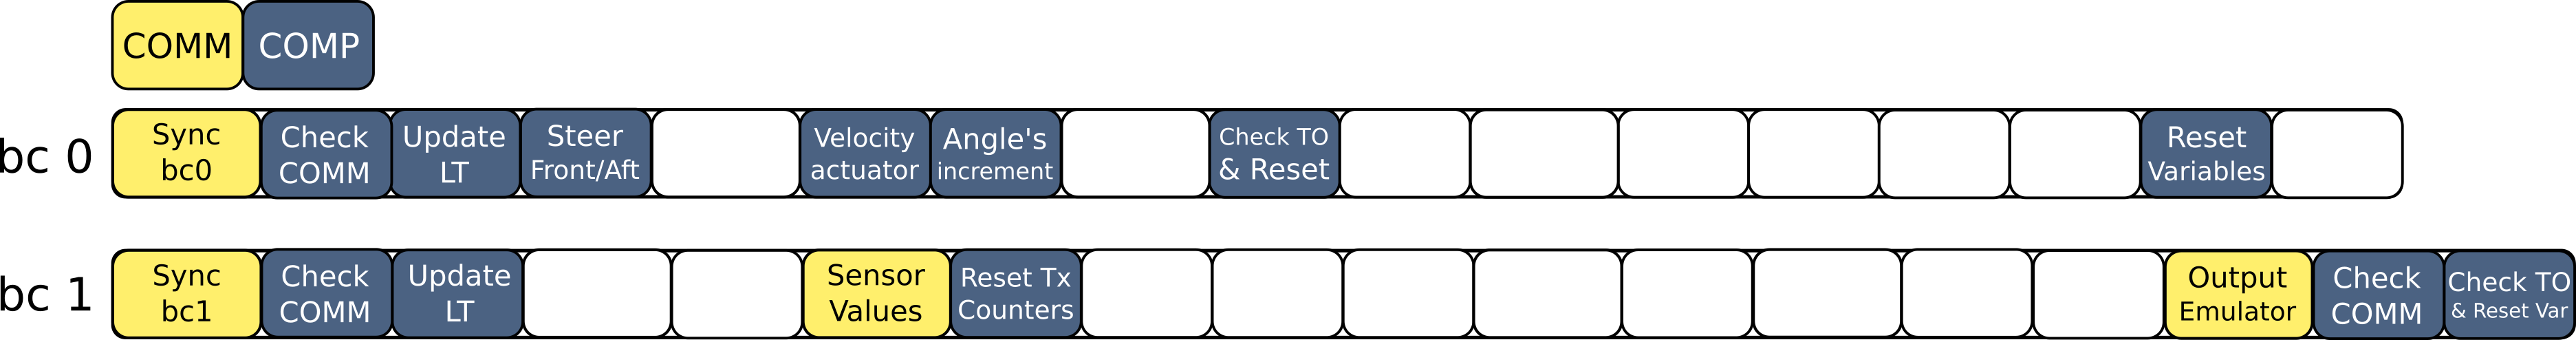
\includegraphics[width=\textwidth]{figures/methodology/vehicle_emulator_matrix_cycle.png}
    \caption{Vehicle emulator matrix cycle. Communication (COMM) tasks are painted in yellow and computational (COMP) tasks are painted in blue.}
    \label{fig:vehicle_emulator_basic_cycle}
\end{figure}

The different operations to calculate the sensor values are performed over the first basic cycle. Empty time slots are left in between operations for every communication task happening in the controller. This way both matrix cycles remain synchronous, considering communication and computational tasks do not necessarily have the same duration. The sensor values are sent during the \textit{Sensor Values} communication task. As it happened in the input generator matrix cycle, after sending the message a \textit{Reset Tx Counters} task activates. The values for the actuators are received with the \textit{Output Emulator} communication task. The last task in the matrix cycle assesses the time out of the reference message and resets the cycle variables before starting over.\\


%%%%%%%%%%%%%%%%%%%%%%%%%%%
\subsection{Overview of the software architecture} \label{sec:software_overview}
The software project is divided into different systems and subsystems. A main overview is pictured in figure (\ref{fig:software_overview}).\\

% include software architecture overview scheme!!
\begin{figure}[h!]
    \centering
    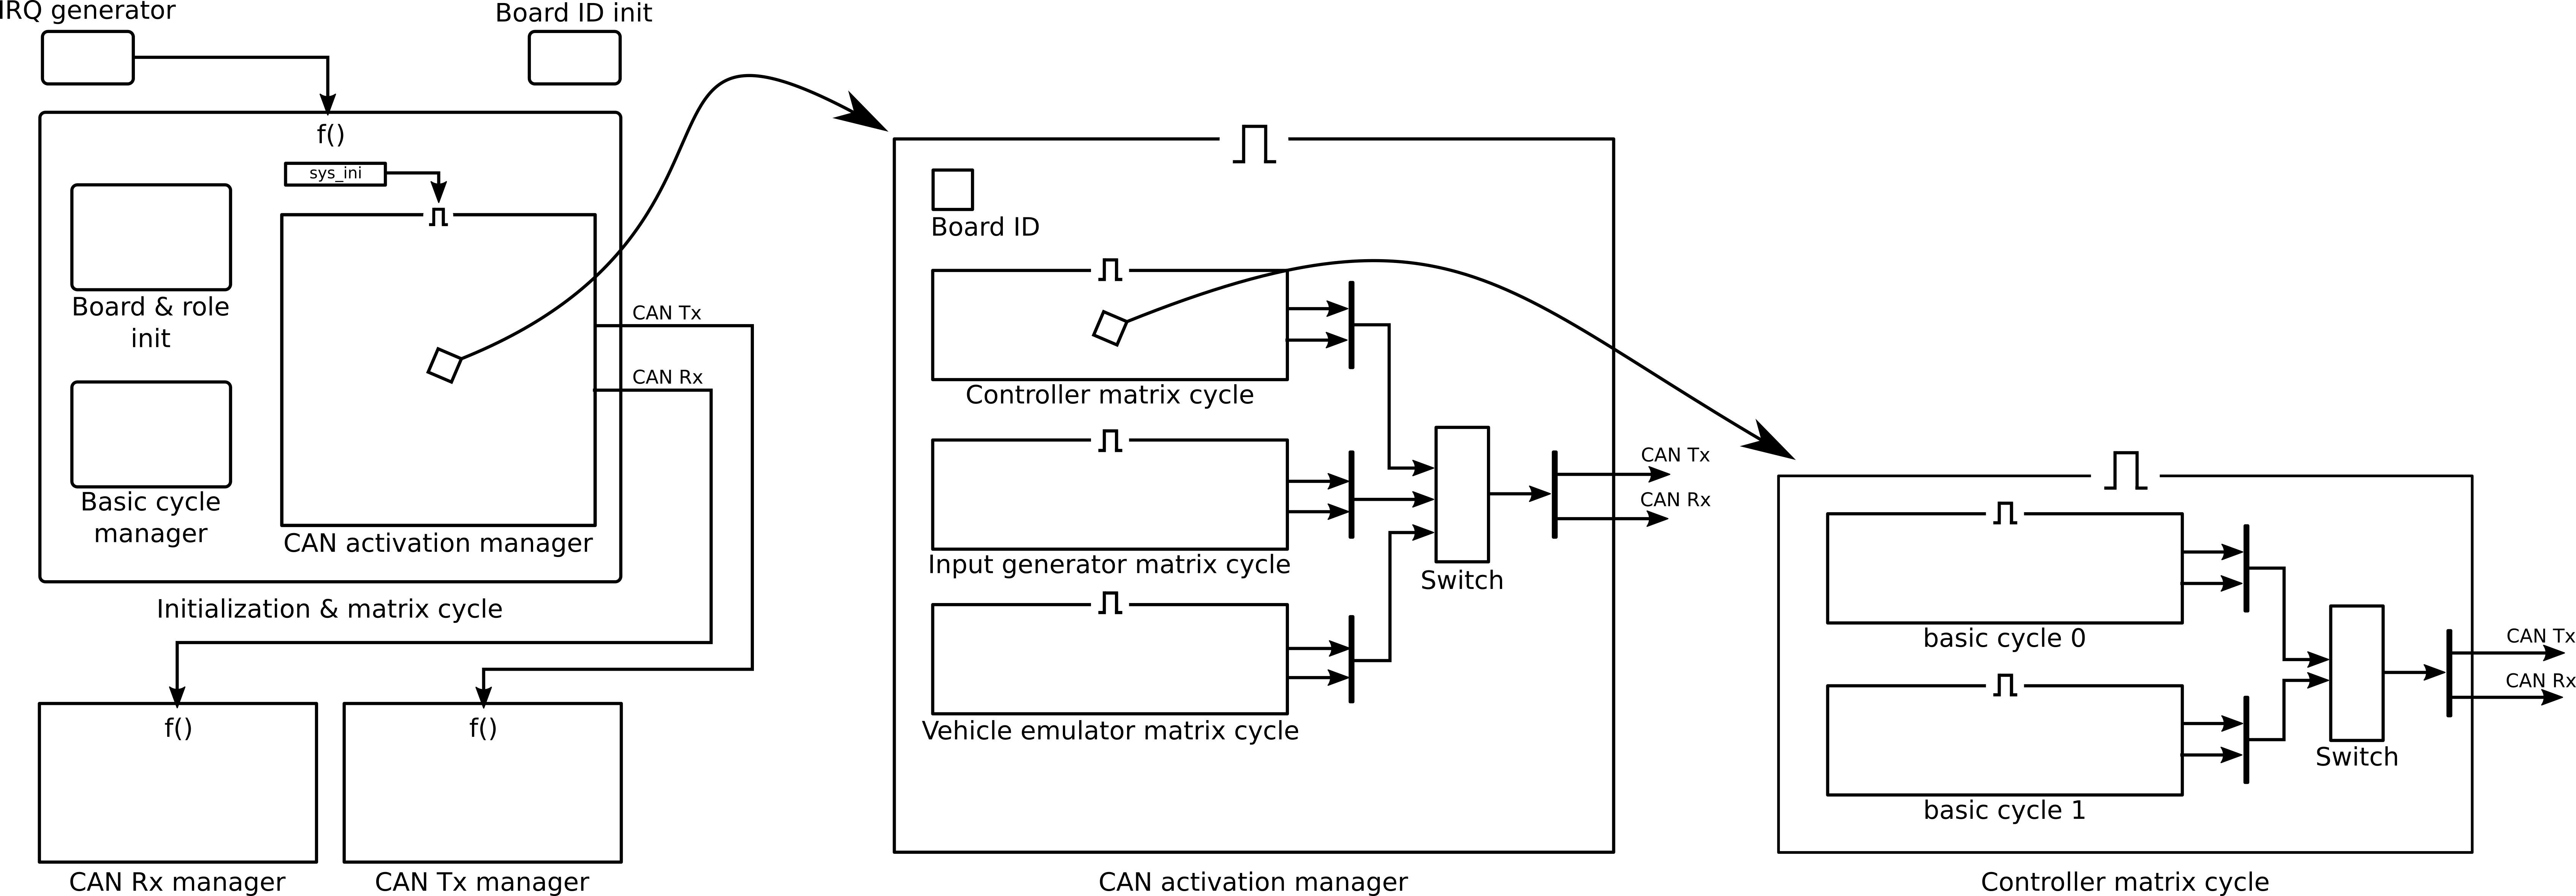
\includegraphics[width=\textwidth]{figures/methodology/software_overview.png}
    \caption{Overview of the software architecture.}
    \label{fig:software_overview}
\end{figure}

Looking at the highest overview of figure (\ref{fig:software_overview}) (leftmost part), at the top-right part, the board ID initialization is presented. Each board performance is differentiated by this number, which is selected by powering a set of digital inputs following binary code. This is the only system presented that is not ruled by the IRQ generator from the top left corner. The IRQ generator is scheduled to generate an interrupt by the hardware clock of the board according to the granularity of the system. This interrupt activates the initialization and matrix cycle system via a function call. Every interruption executes the code inside this system once.\\

If the matrix cycle has not been initialized yet, the board and role initialization subsystem run first. Depending on if the board is part of the controller or not the initialization procedure is different. When they are turned on the controller boards wait for a whole matrix cycle duration waiting for a message. If during this time no message is received, it continues operating as a master and sends the first reference time message, setting the board as initialized and starting the matrix cycle. The input generator and vehicle emulator always wait until they receive the first reference message from the master. If a board is reset during its matrix cycle they start this initialization procedure from the beginning. The main difference between an auto-reset from the boards' side in the matrix cycle and a hard-reset done by the user turning the board off and on again, is that with the auto-reset the board does not lose all the variables information from the matrix.\\

The basic cycle manager is in charge of updating the basic cycle counter every time the local ticks counter reaches the duration of a basic cycle. When the basic cycle is updated, the local time is reset, so the new cycle starts from the beginning. The CAN activation manager is in charge of activating the CAN interface subsystems for transmission (Tx) and reception (Rx) of messages. When looking inside (middle picture of figure (\ref{fig:software_overview})) the three matrix cycles can be visualized. Only one of them is activated depending on the Board ID decided previously. Each matrix cycle subsystem outputs booleans declaring if the CAN Tx or CAN Rx subsystems must be activated during this activation. Only the correct CAN signals are chosen to be output from the CAN activation manager, again depending on the Board ID value.\\

Each matrix cycle subsystem contains the information of the basic cycles of the boards (rightmost picture in figure (\ref{fig:software_overview})). Inside the basic cycle subsystems, each task is declared in a similar fashion, using \textit{enabled subsystems}. This kind of subsystem is only activated when a condition is set to true. The CAN activation manager is only activated if the system has finished its initialization. Only the correct matrix cycle is activated depending on the Board ID value. The basic cycle activated inside the matrix cycle subsystem depends on the basic cycle counter value. Finally, the appropriate task is activated depending on the local time counter, which at each activation will be equal to a value contained in a unique time window of the cycle. If the task being currently active requires sending or receiving a message, the CAN Rx manager or the CAN Tx manager are activated with a function call. These two subsystems are responsible for handling the message buffer to either update it with new information from the CAN network or send the message buffer content to the network. Figure (\ref{fig:software_overview}) shows only one CAN Rx and one CAN Tx manager, but the software has one of these systems per CAN channel.\\


%% <!> CHECK THIS PLEASE!
%% Explain Role ID vs Board ID, Task manager, CAN Tx and CAN Rx, basic cycle
One of the main ideas taken into account when designing the software of this project is hardware agnosticism. This means that the software can run on any STM32-E407 board and still perform any of the component tasks: controller, input generator or vehicle emulator. Furthermore, the controller boards can take either the slave or the master role while the program is running. There is only one version of the software and it is flashed in all the boards without fine-tuning to fit a specific role. The way a board is identified as any of the described components is by hardware connections. There are several pins, from \textit{D2} to \textit{D7}, that are chosen to designate a board ID. Each board has a unique board ID with which the software is able to give it its precise instructions. Another important idea from the software perspective is interfacing. There is a clear distinction between the program systems that are in charge of the board tasks, regardless its role, and the program systems that manage communication between boards. Every time a message is sent or received the software must use the CAN communication interface to perform the message exchange.\\

The characteristic that stands out the most when comparing this thesis software with a more conventional \textsc{Matlab}-Simulink program is how the simulation time is handled. \textsc{Matlab}-Simulink lets the FreeRTOS handle the program execution time by default. The program sample time is defined in its configuration and the software blocks run at that rate. If the sampling frequency is set at 10 kHz (normally the fastest sample frequency in Simulink), the program runs its loops at that frequency. However, for this thesis it has been decided to set the sampling frequency by hardware interrupts with an internal clock of the boards. By relying on an external source for software granularity, the sampling frequency is more reliable as it is not depending on a computer calculation that could either be delayed or accelerated because of processor overhead. The software subsystem in charge of creating the IRQs for the other subsystems is the IRQ generator. This generator sets a stable rhythm for the other parts of the software, creating the notion of the local time of the board. It is also possible to change this sampling frequency to be even faster than Simulink's limit of 10 kHz.\\




%%%%%%%%%%%%%%%%%%%%%%
\subsection{System deployment and testing}
% Introduction to deployment. What can go wrong with system deployment?
When working with a simulation there are factors that are sometimes disregarded that impact the performance of the system when taking it to the real world. This is why deploying the system into a hardware environment to study its behaviour is an important and challenging step. The challenge starts when the simulation falls apart under physical limitations and unexpected problems. In this project, there are already some forecast issues from the design stage, such as the software clashing with the underlying FreeRTOS at high granularity frequencies or the minimum communication delay. The most unexpected limiting event found in this project can be found at the end of section \ref{sec:Results}. Results.\\

This last section of Methodology shares a brief overview of how the system was deployed, presenting the main tools employed. It continues by defining the test case developed to showcase the findings of the project and finishes by listing the measurements and fault injections presented in the Results section.\\

\subsubsection{Deployment}
% Overview on how the system was deployed: prototyping
From the beginning of the Minor Project where this thesis' code started to take shape, the development focused on fast prototyping. Deployment has been done taking small steps with new features and testing that the behaviour was (at least to some extent) as expected. The system was deployed step by step, from a local tick generator to a global time synchronized ensemble of boards. The controller behaviour was tested in a simulation before deploying it to the boards, to ensure that the calculations performed, the communication packaging to send through CAN and vehicle response was coherent with the original Simulink source. The new simulation had the main difference of being executed under a signal interrupt basis instead of using Simulink's software activation. The PID controller gains were first estimated using the Ziegler and Nichols method \citep{ziegler_nichols}, as it is a standard popular method to estimate the gains of a PID controller, and later tuned on according to the system response.\\

The code was developed using \textsc{Matlab}-Simulink model-based design environment, along with HANcoder-1.0 extension. When the code is compiled a '.srec' file is generated, which can be flashed into the STM32-E407 boards using the program Microboot. A detailed electric scheme with the connections between the different boards is presented in appendix \ref{app:hardware_connections}. It is possible to see the system's signal evolution while the boards are running using the HANTune\_build\_68 software. HANTune has a maximum sample frequency of 100 Hz, so, even if it is really useful to check the state of the internal signals of the program, it is not able to record with enough precision everything that happens at the clocks frequency rate, as their ticks are in the order of the kHz. That is why a logic analyzer with a maximum sample frequency of 24 MHz is used to check any event that happens in the software at the level of task activation. The logic analyzer employed is from Az-delivery and counts with 8 digital channels to monitor signals concurrently in real-time. The software used to connect the developer laptop to the logic analyzer is Logic (2.3.37) from \textsc{Saleae}, as it is free, recognizes the logic analyzer automatically and has the option to export the recordings to a '.csv' file. The digital records were processed using python scripts to get some of the results from section \ref{sec:Results}.\\

\subsubsection{Test case definition}
% What do we want to demonstrate in the test case? How we will see that the system is performing good enough?
The test case for this project aims to demonstrate that the vehicle controller can make the vehicle emulator behave according to the values set by the reference generator. Also, it shows that the system is robust under certain failures and the operation continues in spite of them. The operational design domain under which the test case will perform its activities is the following:
\begin{enumerate}
    \item The controller only controls the speed loop of the vehicle. The controller upon it was based was only tested in speed and the controller in this project does not add up any new functionalities.
    \item If a controller board does not receive either a set message (from the input generator) or a sensor message (from the vehicle emulator) it will not perform the calculations for the output. It will raise an alarm and send an error log to the master controller board.
    \item If the vehicle emulator does not receive a message with controller outputs it will remain in the same state as it was and the sensor value transmitted to the controller will remain as zero until a new message is received.
    \item The vehicle emulator will not process the error log received by the controller.
\end{enumerate}
The simplified operation defined for the test case is meant to focus the attention on the redundancy and synchronicity achieved on the controller side. No complex operations were performed outside the controller design as these were considered out of scope.\\

\subsubsection{Measurements and fault injection}
There are five main measurements that assess the synchronicity and correct temporal behaviour of the boards while performing operations.
\begin{enumerate}
    \item The \textbf{granularity}, that shows that the code is activated at a steady pace at the frequency set by the software interrupts.
    \item The \textbf{communication delay} from the moment a message is sent until it is received. This measurement is needed to calculate the ensemble precision.
    \item The \textbf{ensemble precision}, which shows what is the time difference between the slave boards and the time master board in the controller.
    \item The \textbf{tasks execution time}, to get to know how much operational load is in the different tasks of the matrix cycle and define the WCET.
    \item And finally, the \textbf{controller cycle duration}, which is extrapolated from the other measurements.\\
\end{enumerate}
% Discuss what fault injection is going to be performed
When the vehicle emulator got to respond to the set values from the input generator, some fault injection was performed. The tests are mainly focused on the time synchronized model.
\begin{enumerate}
% 1. shutting down a board - the system keeps working
\item The system can keep running even if one of the controller boards is shut down. 
% 2. insertion in the matrix from shut
\item While the system is running, a shutdown controller board must be able to synchronize and engage with the system, resuming normal operation.
% 3. reinsertion in the matrix from failure
\item If a controller board has just stopped being synchronized with the rest of the system it must be able to recognize it and perform an auto-reset, achieving synchronicity again later.
\end{enumerate}
The fault injection is provoked by switching on and off the boards in the ensemble with the wake-up button. When the wake-up button is pressed the board freezes until the wake-up button is pressed again. All the information about the messages lost by the controller boards during the second basic cycle is reflected in the error log that is output to the vehicle emulator along with the actuator values.

%%%%%%%%%%%%%%%%%%%%%%%%%%%%%%%%%%%%%%%%%
%% <<<<<<<<<<<<>>>>>>>>>><<<<<<<<<<<<< %%
%%%%%%%%%%%%%%%%%%%%%%%%%%%%%%%%%%%%%%%%%


\newpage
\section{Results}\label{sec:Results}
%%%%%%%%%%%%%%%%%%%%%%%%%%%%%%%%%%%%%%%%%
The results are divided into the time analysis of the prototype behaviour and the test case results. The first section focuses on the time aspects of the clock activation, the boards' synchronization, the message exchange and the task periods. The second section presents the vehicle emulator response and the boards' behaviour with fault injection.

\subsection{Time analysis}
It is important to assess the time limits and performance of the boards during operation to be aware of the potential of the prototype and emphasize the points where further research is required. This time analysis section presents the measurements performed over the granularity, ensemble precision, communication delay, computational task time and controller cycle duration. Here the results are merely presented and further analysis is held later in section \ref{sec:Discussion}. Discussion.

\subsubsection{System's granularity}\label{sec:granularity}
Every time the hardware clock in each board activates generates a function call to activate the code. A digital output has been toggled every time this has happened, so the difference between two consecutive toggles results in the system granularity. A recording of the granularity over a whole matrix cycle is presented in figure (\ref{fig:granularity_measurement}). The average granularity recorded is $\bar{gr} = 0.10001$ ms, the maximum $gr_{max} = 0.13271$ ms and the minimum $gr_{min} = 0.06983$ ms.\\

\begin{figure}[h!]
    \centering
    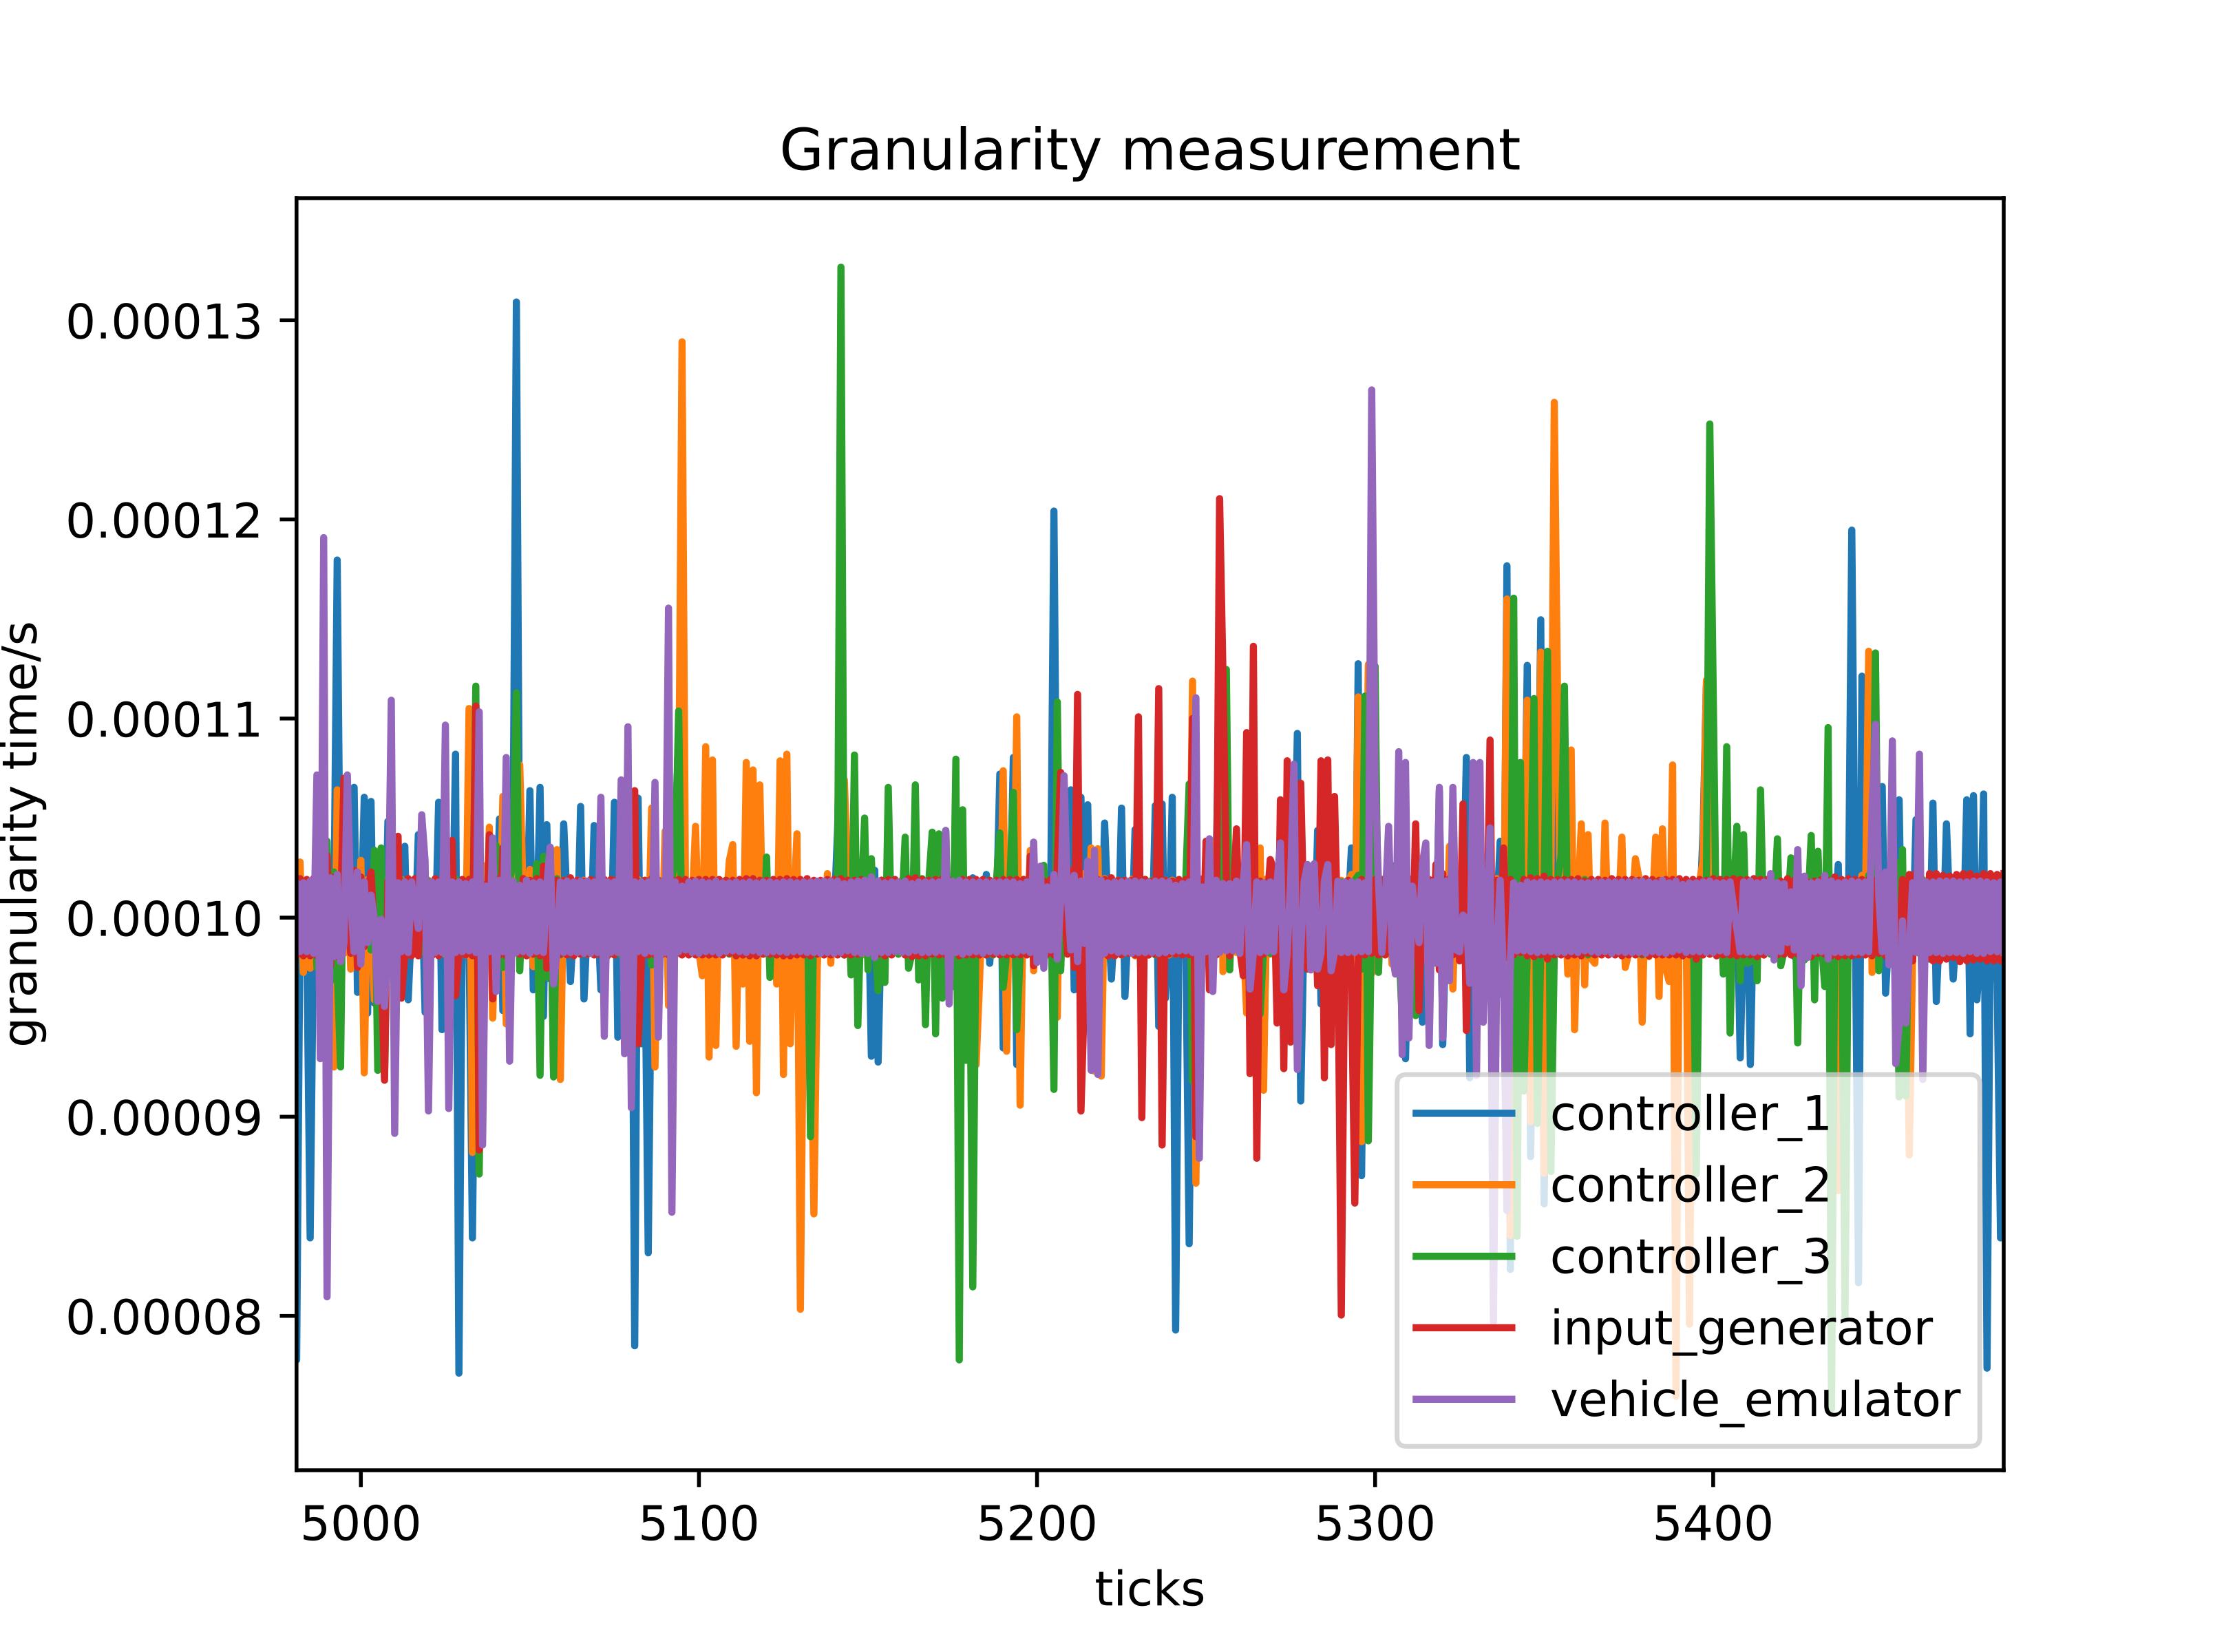
\includegraphics[scale=0.75]{figures/results/granularity_measurement_0_1ms.png}
    \caption{Granularity measurement over a matrix cycle for 0.1 ms granularity.}
    \label{fig:granularity_measurement}
\end{figure}

The granularity employed for the test case is 0.1 ms, the same as the minimum software activation that can be achieved with Simulink. However, this project's software has the option to run faster. Unfortunately, running at 0.07 ms (or below) triggers a clock activation error, as can be observed in figure (\ref{fig:clock_lag_activation}). Instead of always activating every 70 $\mu$s, there are periods of time in which the clock activates every $\sim\,$65.6 ms instead.

\begin{figure}[h!]
    \centering
    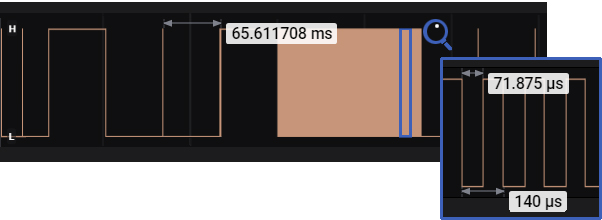
\includegraphics[scale = 0.4]{figures/results/clock_lag_activation.jpg}
    \caption{Measurement portion of the granularity measurement with 0.07 ms granularity with the logic analyzer. The measurement shows the highs (H) and lows (L) of the clock activation. A small portion has been magnified to clarify the frequency of the signals in the solid section.}
    \label{fig:clock_lag_activation}
\end{figure}


\subsubsection{Communication delay}
When a message is transmitted there is some time from the moment the message is sent from one board until it is received by the other. To measure it in an automatized fashion two digital outputs were used: one is toggled when the message is sent at the sender and the other when the message is received at the receiver board. This allows measuring the difference between one event and the next with the logic analyzer. The result found is that the communication delay between boards is around $0.3 \pm 0.1$ ms for both CAN1 and CAN2 channels. This measurement was done using only one message during the transmission in each communication task.


\subsubsection{Ensemble precision}
To check how much out of phase is every board with respect to the global time of the master board the difference in ticks between the moment the synchronization message is expected to be received and when it is actually received is calculated, from now on called desynchronization. This relies on the knowledge of two entities, the time schedule of the board transmitting the message and the communication delay. This last temporal entity is just estimated through observation and it is not a constant value. Also, this desynchronization is used to correct the local time of a board with respect to the master, so the influence of a too-long unexpected communication delay should be minimized. This is why the desynchronization value has been limited to $\pm\,$15 ticks. The average, maximum and minimum values of the desynchronization ticks of the different boards are presented in table (\ref{tab:desync}).

\begin{table}[h!]
\centering
\begin{tabular}{lcccc}
 & \multicolumn{1}{l}{Controller$_2$} & \multicolumn{1}{l}{Controller$_3$} & \multicolumn{1}{l}{Vehicle Em.} & \multicolumn{1}{l}{Input Gen.} \\
AVG & 1 & 2 & 12 & 14 \\
MAX & 15 & 15 & 15 & 15 \\
MIN & -15 & -15 & -14 & -15
\end{tabular}
\caption{Mean desynchronization ticks from synchronization messages from the master and each other board.}
\label{tab:desync}
\end{table}


\subsubsection{Computational tasks time}
The clock activates every some time defined by the granularity of the system, so the whole software is run once again. Before this happens the previous software run should have already finished. Measuring the time elapsed from the moment the code is activated until it finishes all its computations allows to assess how much spare time is there for extra calculations. Figure (\ref{fig:mex}) presents the execution time at each tick during a matrix cycle of every board. The maximum execution time recorded is $et = 0.068$ ms. Adding a 20\% safety margin the estimated WCET is 0.082 ms.

\begin{figure}[h!]
    \centering
    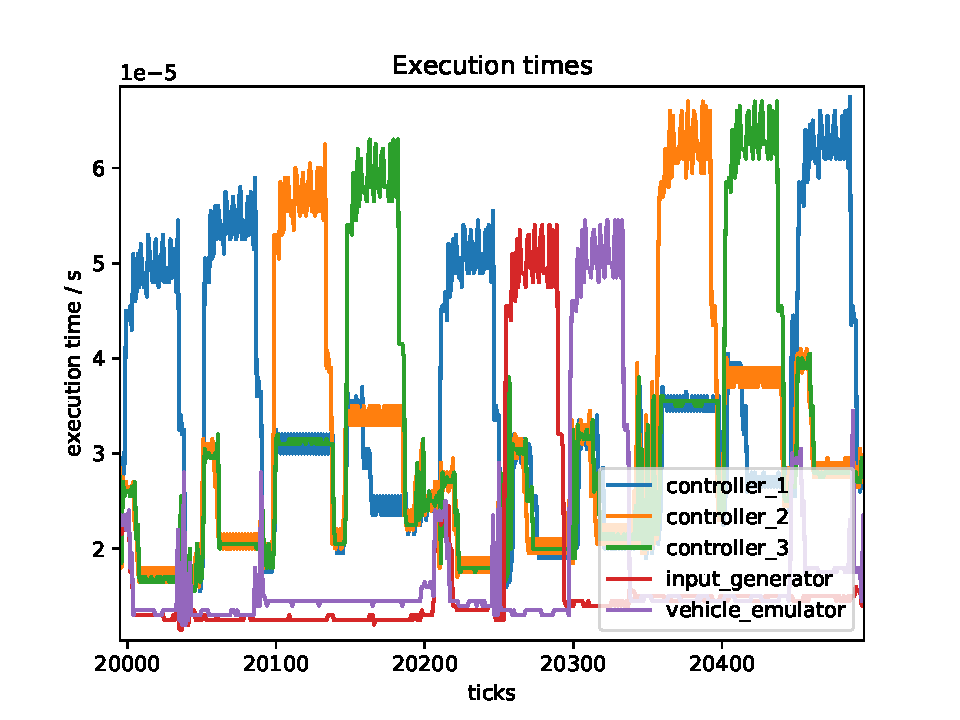
\includegraphics[scale = 0.9]{figures/results/mex_14Jan22_graph.pdf}
    \caption{Execution time of the different boards over a matrix cycle.}
    \label{fig:mex}
\end{figure}


\subsubsection{Controller cycle duration}
% state COMP and COMP durations, each basic cycle duration and matrix cycle duration, in ticks. Relate to granularity and say the controller cycle lasts 50 ms, as proposed by Aart-Jan.
Every computational task in the code has been set at 4 ticks and every communication task at 40 ticks, so according to the matrix cycle presented in figure (\ref{fig:matrix_cycle}) the whole matrix cycle duration is 500 ticks. Every tick, as presented in subsection \ref{sec:granularity}. System's granularity, lasts 0.1 ms, making the whole matrix cycle duration 50 ms. This is the controller cycle duration proposed by the company supervisor of this project Aart-Jan de Graaf to control the vehicle emulator.

%%%%%%%%%%%%%%%%%%%%%%%%%%%%%%%%%%%%%%%%%
\subsection{Test case results}
The main research question of this thesis is answered in this section when presenting the vehicle response of the vehicle emulator when changing the set value at the input generator. A first introductory subsection describes the process followed to choose the speed PID controller gains. In the end, the behaviour of the system with the fault injection is explained and one of the major limitations of the prototype is presented: the missing messages.

\subsubsection{PID gains}
Following the Ziegler and Nichols method, increasing the proportional gain in small steps results in periodic oscillations of the system. When reaching a proportional gain of $k_{pu} = 100$ units in the speed controller, a speed change provoked natural oscillations in the vehicle emulator speed with a period of $T_u$ = 3 s. The formulas to get a response without overshoot are $k_p = 0.2\,k_{pu}$, $k_i = T_u/2$ and $k_d = T_u/8$ \citep{ziegler_nichols_pid}. The proposed integral gain was too strong, so it was manually reduced until the action was reasonable. Just proportional and integral gain worked fine to follow the set signal and reduce the steady-state error, so no derivative control was added. The final PID gains chosen are $k_p = 20$ and $k_i = 0.001$.

\subsubsection{Vehicle response}
The main research question of this report asks if it is possible to deploy a controller in the STM32-E407 boards with Real-Time communication using HANcoder. As presented in figure (\ref{fig:vehicle_response}), it is possible.

\begin{figure}[h!]
    \centering
    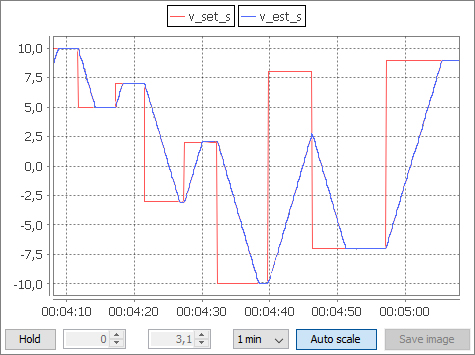
\includegraphics[scale = 0.7]{figures/results/vehicle_response_13Jan22.jpg}
    \caption{Superposition of the vehicle response (v\_est\_s in blue) of the vehicle emulator and the velocity set (v\_set\_s in red) of the input generator.}
    \label{fig:vehicle_response}
\end{figure}

\subsubsection{Fault injection}
As previously presented in the test case operation design description, there are different scenarios in which the prototype must behave as planned to show that the system is robust against communication and board errors. When one of the controller boards is shut down, the other two boards change their roles if necessary so there is one master. If there are no other failures, the two remaining boards will continue to operate and agree in the speed calculations, so the TMR outputs a coherent torque value for the wheels. The error log also shows which board failed. If two boards are shut down the output from the controller remains at $\tau = 0$ Nm and the error log shows the disagreement between the boards and the missing messages. The vehicle emulator remains at the same state while the torque is null. Resuming the operation of a board by just clicking the wake-up button or by reinitializing it again with a hard reset, allows it to synchronize with the master (if there is any) or to take that role.

\subsubsection{Missing messages}
One of the major problems currently limiting the software potential is the missing messages error. While the boards are operating, even though the vehicle emulator works fine and the vehicle response remains stable regardless of this problem, it is possible to see, after enough time waiting, that some messages are sent but not received. Closer inspection with the logic analyzer shows how sometimes messages are sent by a board and, while the receiver board is synchronized, no messages are acknowledged. This problem gets worse if instead of sending several messages only one message is sent every communication task. A fifteen minutes recording example of missed messages during operation is presented in table (\ref{tab:missed_msgs}).

\begin{table}[h!]
\centering
\begin{tabular}{lcccccccccc}
 & \multicolumn{1}{l}{Sync$_0$} & \multicolumn{1}{l}{Vote$_1$} & \multicolumn{1}{l}{Vote$_2$} & \multicolumn{1}{l}{Vote$_3$} & \multicolumn{1}{l}{Sync$_1$} & \multicolumn{1}{l}{Set} & \multicolumn{1}{l}{Sensor} & \multicolumn{1}{l}{Out$_1$} & \multicolumn{1}{l}{Out$_2$} & \multicolumn{1}{l}{Out$_{Contr.}$} \\
Controller$_1$ & x & x & 0 & 0 & x & 194 & 111 & 0 & 0 & x \\
Controller$_2$ & 0 & 0 & x & 0 & 0 & 174 & 140 & x & x & x \\
Controller$_3$ & 0 & 0 & 1 & x & 0 & 154 & 130 & x & x & x \\
Input Gen. & 4 & x & x & x & 3 & x & x & x & x & x \\
Vehicle Em. & 39 & x & x & x & 38 & x & x & x & x & 44
\end{tabular}
\caption{Number of messages not received on each board during fifteen minutes data recording. The 'x' means that message is not meant to be received by that board. During the recording duration Controller$_1$ remained as the master of the ensemble.}
\label{tab:missed_msgs}
\end{table}

The occurrence of this problem seems random and unstable. It has been observed that by reducing the communication tasks period (currently 4 ms) the missing messages increase. The values shown in table (\ref{tab:missed_msgs}) might not be accurate enough of the occurrence frequency of this error but shows in general terms how some roles are more sensitive than others to miss certain messages. More in-depth results of this problem are presented in appendix \ref{app:missing_msgs}. 




%%%%%%%%%%%%%%%%%%%%%%%%%%%%%%%%%%%%%%%%%
%% <<<<<<<<<<<<>>>>>>>>>><<<<<<<<<<<<< %%
%%%%%%%%%%%%%%%%%%%%%%%%%%%%%%%%%%%%%%%%%

\newpage
\section{Discussion}\label{sec:Discussion}
The presented results lead to a series of different questions or missing relationships that are either answered or assessed in this section. These topics are divided into three groups:
\begin{enumerate}
    \item Why is there a limit in granularity and what is causing it? What is causing the maximum execution times? Are granularity and execution-time correlated?
    \item Is the ensemble precision related to the communication delay? Why do input generator and vehicle emulator have bigger desynchronization values?
    \item What is causing the missing messages? Why input generator and vehicle emulator values are far more impacted by this problem? Why is this limiting the software? What other limitations have been found?
\end{enumerate}
After assessing the limitations of the prototype, the discussion leads into section \ref{sec:Conclusion}. Conclusions and recommendations, where some advice is presented about further investigation and improvement of this project's application.

\subsection{Granularity and execution time}
When trying to reduce the granularity of the system to increase the cycle speed we find a limiting granularity time, $gr = 0.07$ ms. This time is close to the maximum execution time required by some of the tasks in the matrix cycle, as seen in figure (\ref{fig:mex}). When the code requires more time to finish its execution than the time left for the next activation, the clock lag activation error from figure (\ref{fig:clock_lag_activation}) triggers.\\

Figure (\ref{fig:mex}) shows the execution time required by every tick in a matrix cycle, so it is possible to compare this to the matrix cycle in figure (\ref{fig:matrix_cycle}) and make a relationship between tasks and execution time. Every high execution time section from this figure corresponds to a communication task in the cycle. The order of communication tasks is: synchronization in basic cycle 0 (controller$_1$), vote 1 (controller$_1$), vote 2 (controller$_2$), vote 3 (controller$_3$), synchronization in basic cycle 1 (controller$_1$), set values (input generator), sensor values (vehicle emulator), output controller 1 (controller$_2$), output controller 2 (controller$_3$) and controller output (controller$_1$). After calmly inspecting this figure in order this consecutive order of tasks is apparent.\\

When comparing figures (\ref{fig:granularity_measurement}) and (\ref{fig:mex}), it is possible to see some similarities that lead to think that they might be correlated. They have been merged together in figure (\ref{fig:mex_gr_comparison}) for better visualization.\\

\begin{figure}[h!]
    \centering
    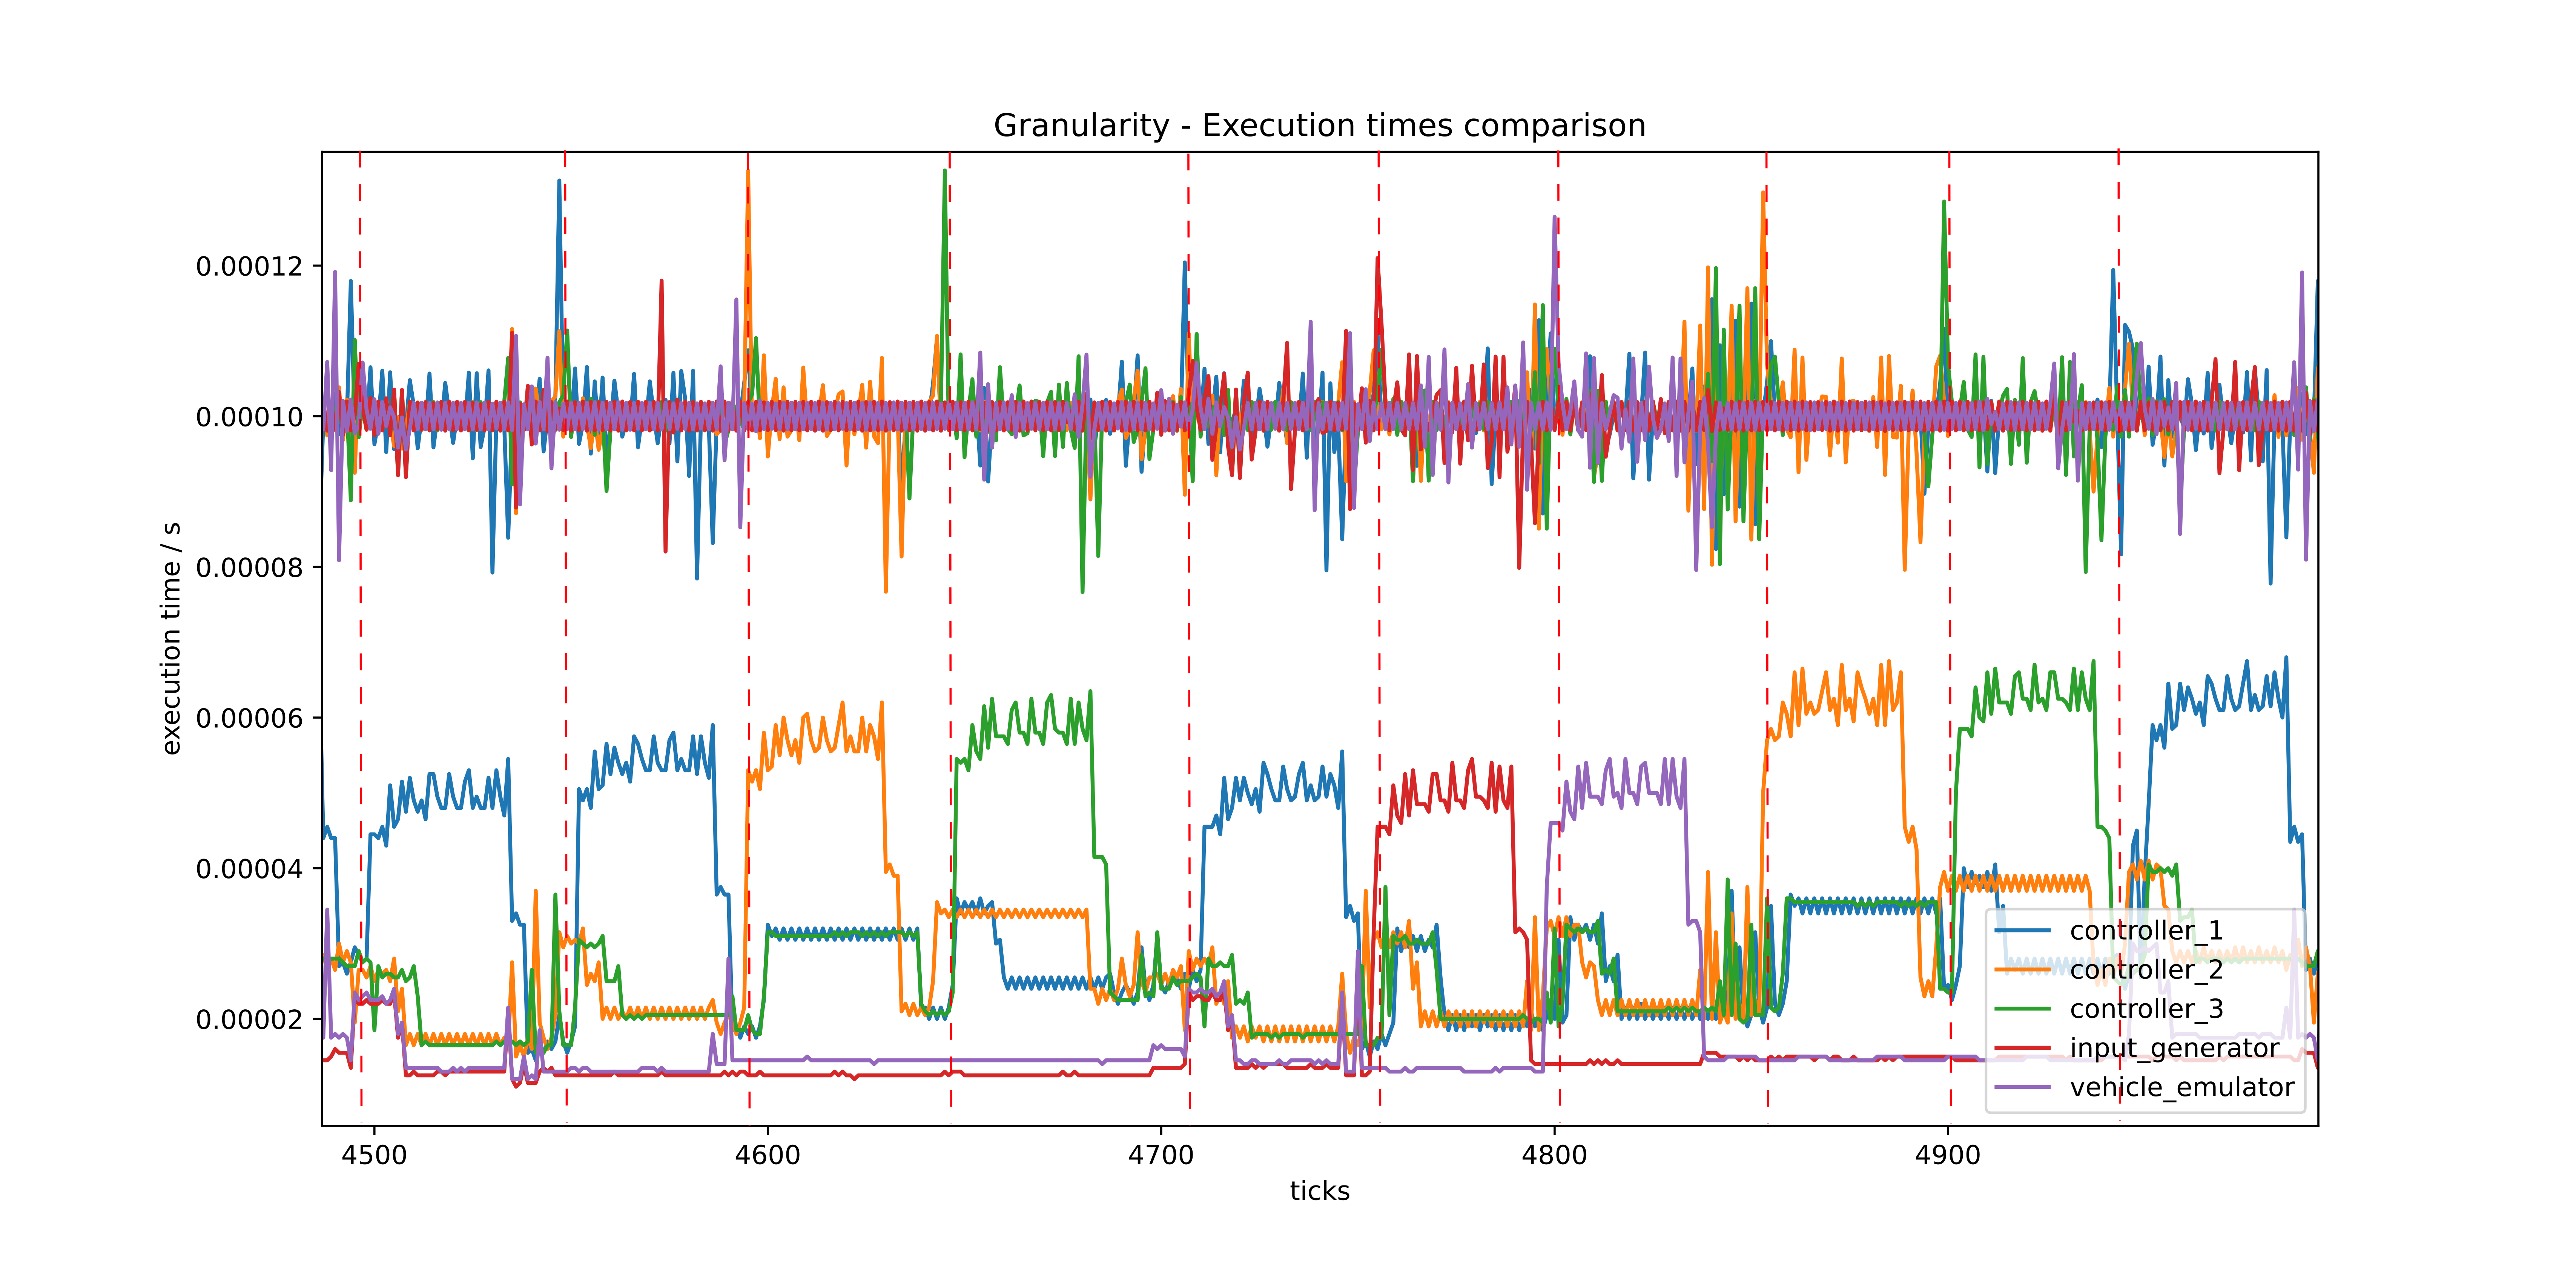
\includegraphics[width=\textwidth]{figures/discussion/mex_gr_comparison.png}
    \caption{Superposition of granularity measurement (top) and execution time measurement (bottom). The vertical dashed red lines help visualize the apparent correlation between the two.}
    \label{fig:mex_gr_comparison}
\end{figure}

With close inspection of figure (\ref{fig:mex_gr_comparison}) it is possible to see that for every peak in the granularity section there seems to be a correspondence to a high execution time section (a red dashed line helps visualize the alignment). Also, by the end of the communication task, there are some low granularity peaks on every board. In the execution time part, between the sensor values task (purple) and the output control 1 task (orange), there is also a spiky section where the controller boards make the calculations for the output to the vehicle emulator. These spikes are also present in the granularity section.\\

All these details matching together guide us closer to the idea that the clock activation is somewhat related to the time each task requires to finish its execution. This is inherently wrong, as choosing the hardware clock was mainly because it is important to be able to have an external source of ticking that will ensure that the deadlines are met regardless of computational load. Also, if the computational load gets close to the tick activation time, the code stops working because of the clock lag activation error from figure (\ref{fig:clock_lag_activation}).\\

However, when looking at the whole picture, it does not seem like such a big problem, because the clock activation seems to be 'recovering' some of the lost time in some parts, so the average cycle duration remains at 50 ms. Moreover, keeping every software activation at a low execution time value ensures that the granularity does not deviate much from its average expected value. The code also allows the user to choose to subdivide a task further inside the computational time window. If it is possible to reduce the execution time at the transmission of messages, the highest granularity peaks would disappear and this would allow choosing lower granularity values without triggering the clock lag activation error. It might be also wise to look into some way of activating the code and the clock so they are decoupled, making the core code more robust and true to the idea of reaching deadlines regardless of computational load.

\subsection{Communication delay and ensemble precision}
There are two ways with which two boards can stop being in sync while continuing their operation. (1) The ticking frequency of both boards could be different enough to desynchronize before the next synchronization message or (2) a sync message could have an unexpected longer delay provoking the receiver to correct its local time to a 'wrong' global time based on the temporal information it received. The granularity analysis points towards discarding option (1), as all the boards present the same average granularity over a longer time than a basic cycle. Option (2) seems to at least be in accordance with the values presented in table (\ref{tab:desync}) for the controller. The average controller slave desynchronization with the master has been found to be 1 or 2 ticks, matching the communication delay found in the communication delay analysis. This is not true for the vehicle emulator and the input generator though.\\

Further research is required to find an explanation on why the desynchronization values for the vehicle emulator and input generator are higher than for the controller boards. The current hypothesis is that, as option (2) suggests, there happens to be a higher amount of longer than expected communication delays in the message exchange with these boards. This does not match the measurements found for the communication delay analysis, but this analysis was done for only one message for every transmission. This leaves the question open: when transmitting several messages per communication task, does the average communication delay between controller and both vehicle emulator and input generator increase? Or is there some other phenomenon provoking the higher desynchronization values? Is this related to the missing messages?

\subsection{Missing messages and limitations}
At the beginning of the project, when messages were lost, it was thought the reason was that the boards participating in the message exchange were out of sync. However, even though this could still be the reason that explains some of the messages lost presented in table (\ref{tab:missed_msgs}), it has been observed that some messages transmitted are just not received, even when the boards are synchronized. If a message is lost at the input generator or the vehicle generator synchronization 0 message reception, these boards reset and wait until a new synchronization message is received. If the message lost error persists for some consecutive basic cycles, as happened in the example from figure (\ref{fig:input_get_missed_msgs}), the board keeps waiting. This means that more messages are missed in the controller end, as the input generator or vehicle emulator are 'just listening' waiting for a sync message to arrive instead of sending the messages that they are supposed to send.\\

\begin{figure}[h!]
    \centering
    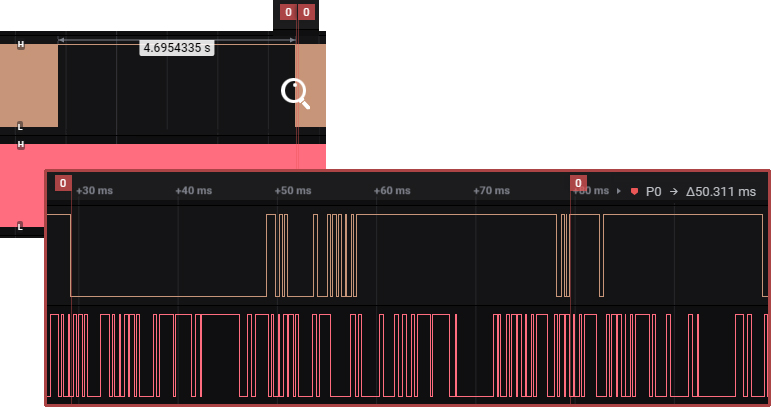
\includegraphics[scale=0.45]{figures/discussion/input_gen_missed_msgs.jpg}
    \caption{Measurement portion of the activation tasks of the input generator (brown) and the master board (red) with the logic analyzer. The magnified portion (bottom right) shows the activating tasks during a matrix cycle right after the input generator resynchronizes. In the not magnified portion (top left) it is possible to see how the input generator stopped operations (reset) during more than 4.6 seconds.}
    \label{fig:input_get_missed_msgs}
\end{figure}

Interestingly, as table (\ref{tab:missed_msgs}) shows, the input generator seems to suffer less from the missing message problem as a receiver than the vehicle emulator, which probably reflects that the problem is not just unique but a combination of several sources that require further research. Possible causes of this problem could range from software problems (code errors that require refinement) to hardware problems. The connections of the boards, even being soldered, have presented some communication troubles and instabilities, probably because the prototype had to go through different trips, making some of the cables get loose and requiring soldering again. Also, due to an error in the initial design of the prototype, the cables used are not twisted pairs as the CAN hardware protocol states. Some electromagnetic interference could also be messing up the message transmission. Moreover, because the CAN channels are not independent of each other, when one of them fails the other does so too. Low-level inspection of the message exchange is required, at both the hardware side, checking where the message is lost, and in the software, inspecting if the message is actually being received but not processed because of desynchronization or other issues. More insight of different parameters influencing the missed messages frequency is presented in appendix \ref{app:missing_msgs}.\\

The main limitation in the current version of the prototype is cycle time. If the boards were able to perform controller operations in less time more sophisticated operations could be built upon them and more communication tasks could be introduced in the matrix to increase the information flux between them. More frequent communication exchange is really important when a higher amount and more precise data is held in the operations that have to undergo the triple modular redundancy.\\

The cycle period is limited by different factors:
\begin{enumerate}
    \item \textbf{Missing messages} are currently not degrading the performance of the prototype for the test case proposed, but it is not acceptable to have missing messages for no reason on a usual basis. Also, it has been observed that by reducing the communication task period the number of missing messages increase. Trying to reduce the current matrix cycle duration by reducing the communication tasks period would increase the missing message occurrence which, in an extreme case, could even put the synchronization of the ensemble at risk.
    \item Another way of reducing the matrix cycle duration is decreasing their \textbf{granularity}. With the current prototype, it is possible to safely increase the board's speed by 20\% (reduce the 0.1 ms ticks to 0.08 ms), but it would be desirable to increase the speed even further, as the software limit is far beyond. Due to initial tests performed during the Minor Project, it is suspected that it is possible to reduce granularity below 0.05 ms without having the FreeRTOS clashing influence in the software.
    \item Requiring the \textbf{role election} during basic cycle 0 is another important drawback. A whole basic cycle (currently being almost half of the whole matrix cycle) is required for the controller boards to acknowledge the time master board during that cycle. It would be important to either change the way CAN communication is managed with the CAN blocks in HANcoder so it is possible to follow the TTCAN protocol, as suggested before in section (\ref{sec:method_master_slave_strategy}), or think of a more efficient way of handling the role allocation in the controller.
\end{enumerate}

Unravelling the source of the missing messages, finding a way of reducing the computational load during transmission tasks and improving the management of the role allocation at the controller could allow the prototype to reach a higher level of performance. If the cycle period could be reduced to its physical limits (minimum communication delay in hardware and FreeRTOS frequency limitation in software) the platform developed in this project could be employed as a basis for future research and more complex Real-Time controllers.


%%%%%%%%%%%%%%%%%%%%%%%%%%%%%%%%%%%%%%%%%
%% <<<<<<<<<<<<>>>>>>>>>><<<<<<<<<<<<< %%
%%%%%%%%%%%%%%%%%%%%%%%%%%%%%%%%%%%%%%%%%

\newpage
\section{Conclusion and recommendations} \label{sec:Conclusion}
It has been shown that it is possible to deploy a controller in the STM32-E407 boards with Real-Time communication using HANcoder. The deployed controller is made of three boards to perform triple modular redundancy with the calculations of the output to the actuators. The prototype counts with two more boards, one for the input generator and another one with the vehicle emulator. As proposed by the company supervisor Aart-Jan de Graaf, a controller cycle of 50 ms is enough to control the speed loop of the vehicle emulator, obtaining a reasonable response. The concept is fully-redundant, as there is no fragile point in the design where one single failure provokes the system to stop operation.\\

Even though the system works fine for the proposed test case, some issues limit the potential of the prototype. The following recommendations aim to put the focus on the current most important topics that prevent the system from performing at its full capacity:
\begin{enumerate}
    \item Make the connections between the boards new again with twisted pair cables as stated in the CAN hardware protocol. Check the CAN communication between the boards with the new connections and ensure they are safe and stable.
    \item Decouple the CAN channels in the HANcoder software so they are independent of each other. The current HANcoder blocks do not offer redundant communication independent channels.
    \item If the problem of the missing messages persists, investigate its source by analyzing the message path, from the transmitter to the receiver. Identify at which point the message is lost, as the problem could be hardware, software or a combination of both. Recording the variable's information within the program for later processing could help with system diagnosis.
    \item Minimize the computational load during the message transmission. This will allow reducing the granularity of the system.
    \item Simplify the master-slave election policy, as it currently requires a whole basic cycle. It can be shortened by changing the way the CAN blocks of HANcoder handle the messages so they fit better the specification from the TTCAN.
\end{enumerate}

The main objective of assessing these issues is to reduce the time required by the controller boards to perform the calculations during the controller cycle. All these time shortening proposals would save time to do other essential activities needed in more complex controller projects. Every time a board has to exchange information with another board it is limited by the bandwidth of the CAN channel. If every message requires less time to be transmitted safely and the whole controller cycle has more free time to exchange information, the Time-Triggered schedules would not be as limited as the one proposed for this project.\\

This project has shown that it is possible to build a Real-Time controller using HANcoder. The current prototype can already be used as a template for a fully-redundant distributed embedded Real-Time application but more research is advised to make it reach its utmost potential and be a useful tool to solve technological problems in the industry.


%%%%%%%%%%%%%%%%%%%%%%%%%%%%%%%%%%%%%%%%%
%% <<<<<<<<<<<<>>>>>>>>>><<<<<<<<<<<<< %%
%%%%%%%%%%%%%%%%%%%%%%%%%%%%%%%%%%%%%%%%%


\newpage
%% Bibliography %%%%%%%%%%%%%%%%%%%%%%%%%%%%%%%
% \bibliography{references}

\printbibliography[title=Bibliography]
\addcontentsline{toc}{section}{\protect\numberline{}Bibliography}

%%%%%%%%%%%%%%%%%%%%%%%%%%%%%%%%%%%%%%%%%%%%%%%
\newpage
\appendix

%%%%%%%%%%%%%%%%%%%%%%%%%
\section{Vote criteria} \label{app:vote_criteria}
%% include vote criteria flowchart!!
The vote decision computational task in the controller matrix cycle follows the criteria from figure (\ref{fig:vote_criteria}).
\begin{figure}[h!]
    \centering
    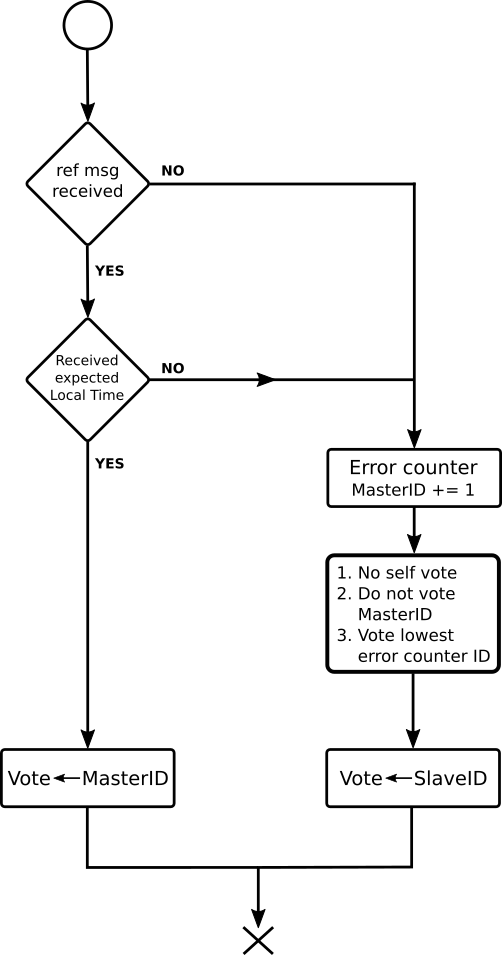
\includegraphics[width=0.5\textwidth]{figures/methodology/voting_decision_making.png}
    \caption{Flowchart of the voting decision logic when casting a vote for the time master. If the reference message received from the master corresponds with the expected Local Time, the vote is cast for the same master board. If any of the other conditions were not set the error counter for the board being the master is increased by one and another board is voted to be the new master. There are three conditions when selecting the vote for a slave board: (1) a board cannot vote itself, (2) a board cannot vote a master that has failed and (3) the vote should be for the slave board with the lowest error counter registered.}
    \label{fig:vote_criteria}
\end{figure}



%%%%%%%%%%%%%%%%%%%%%%%%%%%%%%%%%%%%%%%%%%%%%%%%%%%%%%%
\newpage
\section{Hardware connections} \label{app:hardware_connections}
% Explain what things shall be connected by default and discuss available connections for debugging and testing.
The main connections among the boards are those setting the CAN communication channel. Each board is connected to two CAN transceivers (one per CAN communication channels) using the 3V and ground pins along with pins 3 and 4 for reception and transmission respectively for CAN communication channel 1 and pins D11 for reception and D1 for transmission for CAN communication channel 2.\\

Apart from CAN communication, there are also connections regarding the boards' software functionality. Applying 5V voltage to pins D2 to D7, combining them using the binary base, it is possible to assign different ID numbers to each board. An electric scheme graphically showing all the connections is pictured in figure (\ref{fig:electric_scheme}).\\

\begin{figure}[h!]
    \centering
    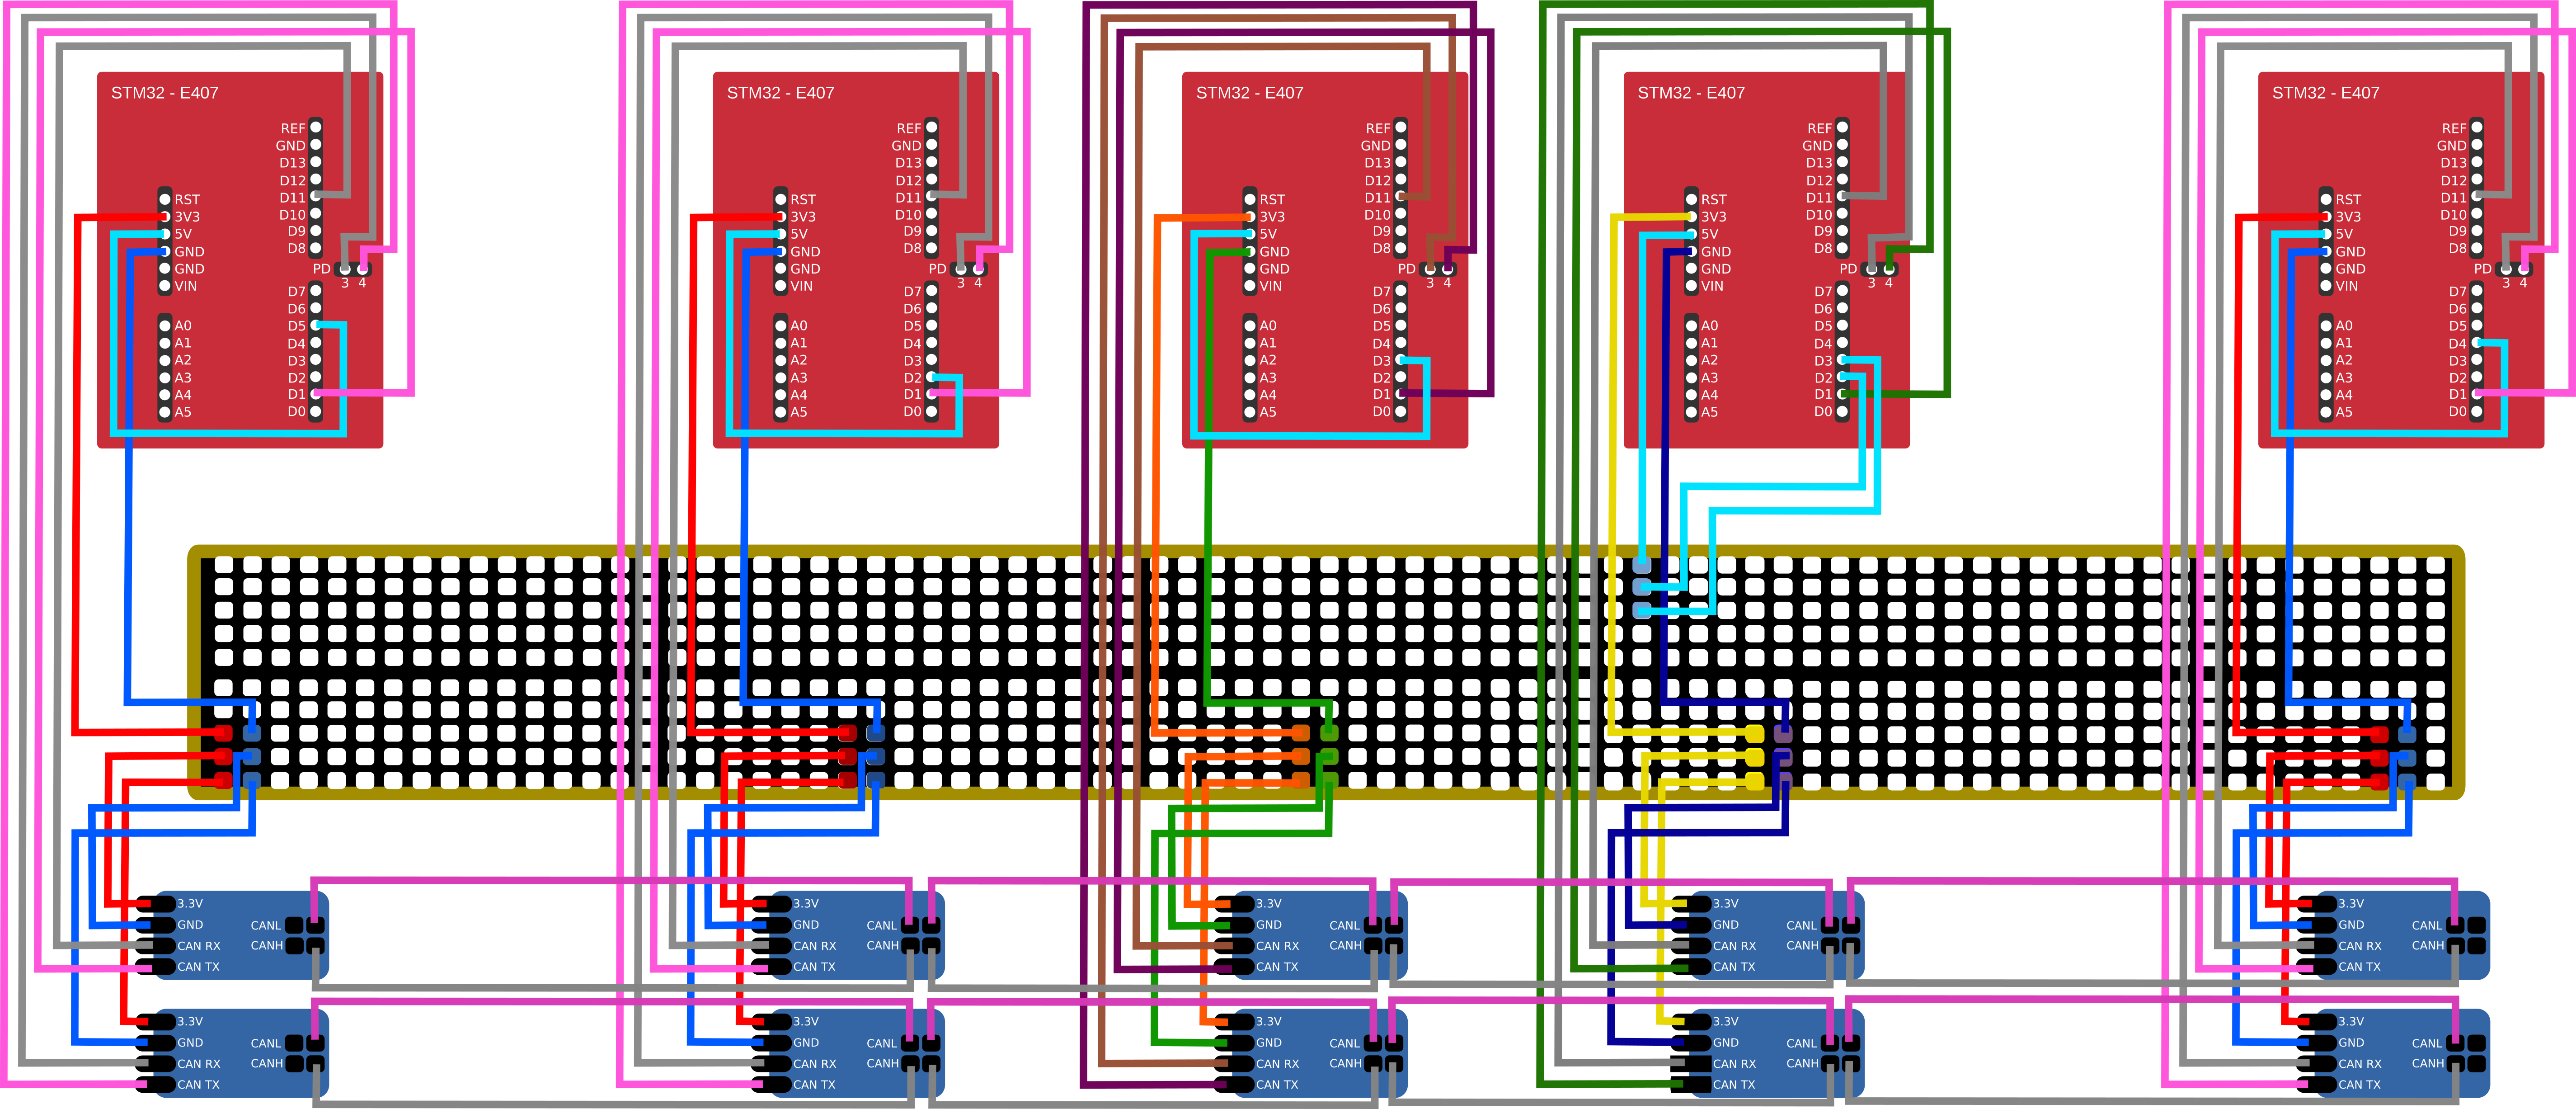
\includegraphics[width=\textwidth]{figures/methodology/electric_scheme_lowres.png}
    \caption{Basic electric scheme of the system with CAN communication and ID connections.}
    \label{fig:electric_scheme}
\end{figure}

% Specify the connections for monitoring and the devices sample time.
Monitoring and testing are done with HANTune. It is possible to connect each board with the developer's laptop using a USB connection. This way the board gets power and HANTune can establish a connection to access all the Simulink signal values. It also allows changing parameters during running time. However, connecting with HANTune requires extra processing by FreeRTOS to manage the communication, so connecting when the hardware interrupts are too frequent may make the system crash. Moreover, HANTune has a limited sample time of 100 Hz, so it is not possible to monitor properly the signals with a high rate of change. That is why HANTune is used to monitor the most steady signals in the system and change the input generator parameters.\\

The system hardware interrupts run faster than HANTune sample time, so to check that the tasks of the matrix cycle are being activated in the appropriate moment a logic analyzer is used. It can be connected to output pins A0 to A5 and D8 to D13 of each board to up to eight channels and it runs with a sample time of up to 24 MHz. When an interesting event in the system happens the pin is toggled, so a digital signal is read by the logic analyzer. This way it is possible to verify the time consistency of the ensemble.



%%%%%%%%%%%%%%%%%%%%%%%%%%%%%%%%%%%%%%%%%%%%%%%%%%%%%
\newpage
\section{Controller operations} \label{app:controller_operations}
% Controller equations
The controller starts estimating the steer front and aft angles from the wheel angles information provided by the sensors.
\begin{equation}
\begin{split}
    \delta_{f\,est} = \int{ \frac{(\dot{\theta}_{fr\,act}R_{fr} - \dot{\theta}_{fl\,act}R_{fl})}{T_{lf}} \textrm{d}t}\\
    \delta_{a\,est} = \int{ \frac{(\dot{\theta}_{ar\,act}R_{ar} - \dot{\theta}_{al\,act}R_{al} )} {T_{la}} \textrm{d}t}
\end{split}
\end{equation}
where $\delta_{f\,est}$ and $\delta_{a\,est}$ are the steering front and aft angles, respectively. Every $\dot{\theta}_{act}$ corresponds to the angle rate of one of the wheels and the $R$ variables are the radii from each wheel to its axis. $T_{lf}$ and $T_{la}$ are the torques at the front and aft of the vehicle.\\

With the estimation of the steering angles it is already possible to calculate the torque at each wheel with the first PID controller.
\begin{equation}
\begin{split}
    \tau_{fr\,out} & = k_p(\delta_{f\,set} - \delta_{f\,est}) + k_i\int{(\delta_{f\,set} - \delta_{f\,est})\textrm{d}t} + k_d \frac{\textrm{d}(\delta_{f\,set} - \delta_{f\,est})}{\textrm{d}t}\\
    \tau_{fl\,out} & = - \tau_{fr\,out}\\
    \tau_{ar\,out} & = k_p(\delta_{a\,set} - \delta_{a\,est}) + k_i\int{(\delta_{a\,set} - \delta_{a\,est})\textrm{d}t} + k_d \frac{\textrm{d}(\delta_{a\,set} - \delta_{a\,est})}{\textrm{d}t}\\
    \tau_{al\,out} & = - \tau_{ar\,out}
\end{split}
\end{equation}
where each $\tau_{out}$ variable is the torque at each corresponding wheel, $k_p$, $k_i$ and $k_d$ are the proportional, integral and derivative gains of each controller and $\delta_{set}$ is the steering angle set by the reference generator, either at the front or at the aft.\\

The inputs to the vehicle controller also allow it to estimate the speed of the vehicle $v_{est}$.
\begin{equation}
    v_{est} = \frac{\dot{\theta}_{fr\,act} R_{fr} + \dot{\theta}_{fl\,act} R_{fl} + \dot{\theta}_{ar\,act} R_{ar} + \dot{\theta}_{al\,act} R_{al}}{4}
\end{equation}

Using the second PID controller, it is possible to calculate the control effort speed $v_{ctr\,eff}$.
\begin{equation}
    v_{ctr\,eff} = k_p(v_{set} - v_{est}) + k_i\int{(v_{set} - v_{est})\textrm{d}t} + k_d \frac{\textrm{d}(v_{set} - v_{est})}{\textrm{d}t}
\end{equation}

Lastly, the torque sent to the actuators is each of the $\tau_{set}$ variables, one for each wheel.
\begin{equation}
\begin{split}
    \tau_{fr\,set} & = \tau_{fr\,out} + v_{ctr\,eff}\\
    \tau_{fl\,set} & = \tau_{fl\,out} + v_{ctr\,eff}\\
    \tau_{ar\,set} & = \tau_{ar\,out} + v_{ctr\,eff}\\
    \tau_{al\,set} & = \tau_{al\,out} + v_{ctr\,eff}
\end{split}
\end{equation}
The derivatives and integrals are handled following the definitions from appendix \ref{app:der_int_def}.


%%%%%%%%%%%%%%%%%%%%%%%%%%%%%%%%%%%%%%%%%%%%%%%
\newpage
\section{Derivative and integral definitions}\label{app:der_int_def}
% Derivative definition
The derivative of a value received can be performed if the last value is still stored. The approximation used is,
\begin{equation*}
    \frac{\textrm{d} y}{\textrm{d} t} \approx \frac{\Delta y}{\Delta t} = \frac{y_2-y_1}{t_2-t_1}
\end{equation*}
where $y_1$ is the previous value of $y$ received at $t_1$ and $y_2$ is the current value of $y$ received at $t_2$. This approximation is better the smaller is $\Delta t$. In this project, $\Delta t$ corresponds to the granularity of the system.\\

% Integral definition
Following the rule that a two-dimension integral is the area under the curve, it is possible to approximate the result by using the trapezoidal rule with the received values every iteration.
\begin{equation*}
    integral\, +=\, \frac{y_2 + y_1}{2}(t_2 - t_1)
\end{equation*}
This approximation is also better the smaller is the difference in time when the signals were received. This method requires to store the previous value of the signal $y_1$ and its time $t_1$ and also the accumulative sum of the variable $integral$.\\

All the operations are just basic sums and products so it is possible to group them in time windows with a specific task and similar computational load. The only limitation when designing a computational task is that it shall require less computational time than a local tick. This is later checked with measurements presented in section \ref{sec:Results}.Results.


%%%%%%%%%%%%%%%%%%%%%%%%%%%%%%%%%%%%%%%
\newpage
\section{Vehicle emulator operations}\label{app:vehicle_emulator_operations}
The following equations are the ones employed to make the calculations in the vehicle emulator. These calculations include the steer angle rates for the front $\dot{\delta}_f$ and aft $\dot{\delta}_a$ parts of the vehicle and the velocity of the actuators $v_{act}$, which are needed for the calculations of the wheel angle displacement $\theta$ of each wheel. Starting with the steering rates:

% vehicle emulator equations
\begin{equation}
    \begin{split}
        \dot{\delta}_f = \int{\left( \frac{\tau_{fr\, set}}{R_{fr}} - \frac{\tau_{fl\, set}}{R_{fl}} \right) \frac{T_{lf}}{I_f} \textrm{d}t}\\
        \dot{\delta}_a = \int{\left( \frac{\tau_{ar\, set}}{R_{ar}} - \frac{\tau_{al\, set}}{R_{al}} \right) \frac{T_{la}}{I_a} \textrm{d}t}
    \end{split}
\end{equation}
where $I_f$ and $I_a$ are the moments of inertia at the front and aft parts of the vehicle.\\

The actuator velocity is calculated as follows,
\begin{equation}
    v_{act} = \int{ \left( \frac{\frac{\tau_{fr\, set}}{R_{fr}} + \frac{\tau_{fl\, set}}{R_{fl}} + \frac{\tau_{ar\, set}}{R_{ar}} + \frac{\tau_{al\, set}}{R_{al}}}{m_v} \right) \textrm{d}t}
\end{equation}

And the wheel angle displacements are calculated this way,
\begin{equation}
    \begin{split}
        \theta_{fr} & = \int{\left( v_{act} + \frac{\dot{\delta}_f T_{lf}}{2} \right) \frac{1}{R_{fr}} \textrm{d}t}\\
        \theta_{fl} & = \int{\left( v_{act} - \frac{\dot{\delta}_f T_{lf}}{2} \right) \frac{1}{R_{fl}} \textrm{d}t}\\
        \theta_{ar} & = \int{\left( v_{act} + \frac{\dot{\delta}_a T_{la}}{2} \right) \frac{1}{R_{ar}} \textrm{d}t}\\
        \theta_{al} & = \int{\left( v_{act} - \frac{\dot{\delta}_a T_{la}}{2} \right) \frac{1}{R_{al}} \textrm{d}t}
    \end{split}
\end{equation}

Derivatives and integrals are handled the same way as in the controller operations. 


%%%%%%%%%%%%%%%%%%%%%%%%%%%%%%%%%%%%%%%%%%%%%%%%%%%%%%%%%%%
\newpage
\section{Message coding/decoding in the CAN communication}\label{app:float2uint8}

CAN communication allows for the transmission of bytes of unsigned integer data. To transmit float numbers it is necessary to code the information before the transmission and decode it at the receiving end. An example of this encoding is presented in figure (\ref{fig:coding}).

\begin{figure}[h!]
    \centering
    
\includegraphics[width=\textwidth]{figures/coding.png}
    \caption{Eight-bit data binary encoding example. The most significant bit (red) corresponds to the sign of the number (0 is positive). The grey bits correspond to the integer part of the number and the blue bits to the decimal part. This number, 67 in binary, originally represents +4.1875.}
    \label{fig:coding}
\end{figure}

To understand how the coding works it is possible to see the example from figure (\ref{fig:coding}). This could be a data value from a torque variable. Torque variables in the controller have a range of [-5, 5]. The absolute value of the integer part of the float number requires a maximum of three bits to be represented in binary ($5_{10} = 101_2$). This means that using a bit for the sign and three bits to represent the integer part, the remaining four bits can be used to represent the decimal part of the number.\\

Using +4.2315 as an example, the sign (+) is considered as 0 and the integer part is 4. The remaining question is how to represent the decimal part 0.2315 with a precision of four bits. The resolution of the number with four bits decimal point is $2^{-4} = 0.0625$, so dividing $0.2315$ over the resolution $0.0625$, the fixed result is 3 (11 in binary base). Lastly, the three numbers are summed up together taken into account their weight in the byte value: $0 \times 2^{7} + 4 \times 2^4 + 3 = 67$.\\

Knowing the precision (bits for the decimal part) used to code the number it is easy to decode it back to its original value in the receiving end.

%%%%%%%%%%%%%%%%%%%%%%%%%%%%%%%%%%%%%%%%%%%%%%%%%%%%%%%%%%%
\newpage
\section{Missing messages error further analysis}\label{app:missing_msgs}
The missed messages have been measured for approximately fifteen minutes time using different parameters. This will hopefully give a deeper insight on different elements that can be provoking this issue.

\subsection{System information exchange and total number of messages sent}
The matrix cycle has a total of ten communication tasks:
\begin{enumerate}
    \item sync0, the reference message sent by the time master at the beginning of the first basic cycle and received by all other boards. The time master has been board$_1$ in all the measurements presented in this appendix.
    \item vote1, the message sent from board$_1$ to the other controller boards with the vote information.
    \item vote2, the message sent from board$_2$ to the other controller boards with the vote information.
    \item vote3, the message sent from board$_3$ to the other controller boards with the vote information.
    \item sync1, the reference message sent by the time master at the beginning of the second basic cycle and received by all other boards.
    \item set, the message with the set values from the input generator to the controller boards.
    \item sensor, the message with the sensor values from the vehicle emulator to the controller boards.
    \item out1, the message from board$_2$ to the time master with the controller calculations.
    \item out2, the message from board$_3$ to the time master with the controller calculations.
    \item outctrl, the message from the time master to the vehicle emulator with the actuator values and the error log.
\end{enumerate}
The number of missed messages is the total number of times one of these communication tasks has not been acknowledged. During a task several copies of a message are sent through both channels, CAN1 and CAN2. If none of the copies sent is received, the message is counted as lost. The total number of messages sent during a matrix cycle is equal to the number of different communication tasks. A matrix cycle lasts for $50\,$ms, so there are $1200\,$messages/min of each kind. Taking into account that the measurement time was $15\pm1\,$minutes, the total number of messages sent of each different kind is $18000\pm1200\,$messages. When increasing or reducing the COMM period the matrix cycle duration also changes. For COMM = $30\,$ticks the matrix cycle duration is $40\,$ms and for COMM = $50\,$ticks the matrix cycle duration is $60\,$ms, so the amount of messages sent is $22500\pm1500\,$messages and $15000\pm1000\,$messages, respectively.\\

\subsection{Missed messages variability}
When repeating the missed messages measuring with the same parameters, we observe some intrinsic variability in the results. The parameters chosen are COMM = $40\,$ticks, $\phi_1 = 5\,$ticks and $\phi_2 = 5\,$ticks, with a baud rate of $1\,$Mbit/s. An analysis of five measurements with the mean, standard deviation, maximum and minimum of every different board misses for every different message is presented in figure (\ref{fig:mss_msgs_var}).

\begin{figure}[h!]
    \centering
    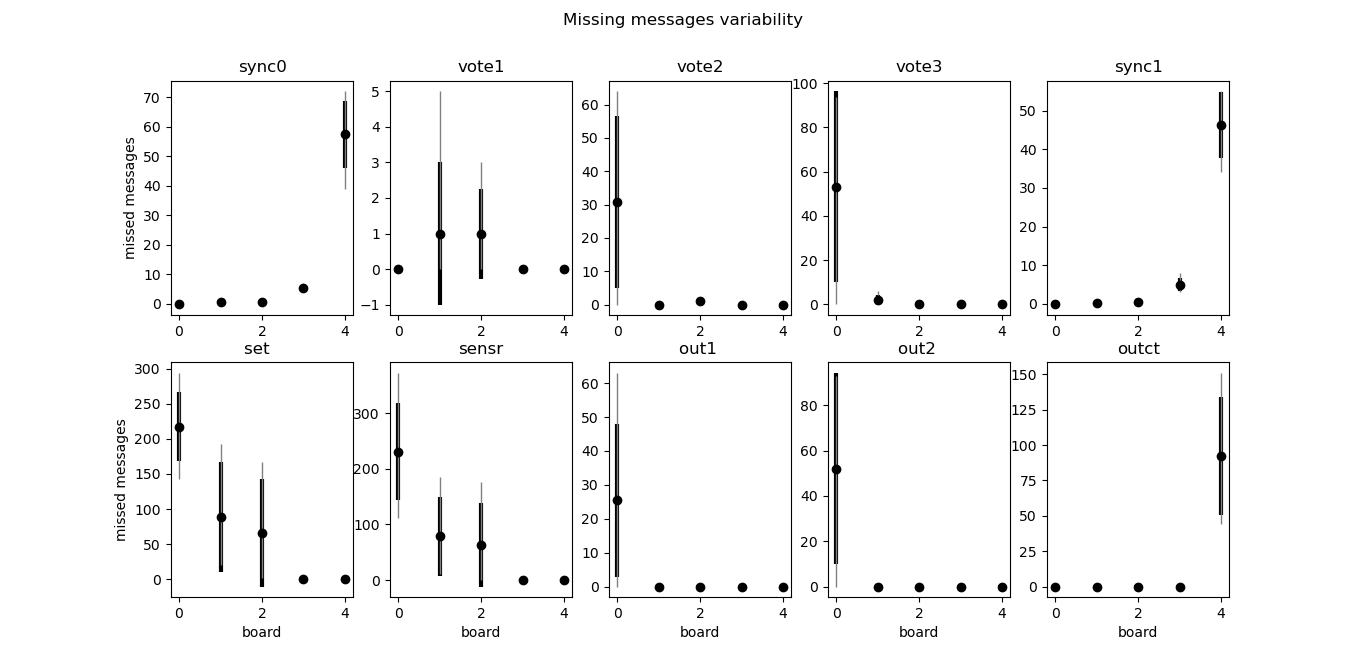
\includegraphics[width=\textwidth]{figures/missing_msgs/missed_msgs_variability_analysis.png}
    \caption{Mean (dot), standard deviation (darker bar) minimum and maximum found for five different measurements of the missed messages for every board at the reception of each different message. Each dot in each subfigure represents a board, from left to right, board$_1$, board$_2$, board$_3$, input generator and vehicle emulator.}
    \label{fig:mss_msgs_var}
\end{figure}

In figure (\ref{fig:mss_msgs_var}) it is possible to see that the missing messages of different boards for some of the messages present a high variability. For example, board$_1$ has been observed to miss between 0 and more than 60 messages when listening to vote2 message. This variation analysis sets some background to understand that making a single recording with a particular set of parameters that shows a low amount of messages missed does not mean the missing chance is necessarily always low for that particular configuration.

\subsection{Influence of different parameters}
As already stated in the discussion of the report, the messages could be missed for different reasons. When thinking about parameters that could be changed in the software that could influence the missing rate the communication period could be important. Sending more copies of a message during a task with a longer communication period or reducing the communication time with a shorter period could change the miss chance. A single recording for three different COMM times is presented in figure (\ref{fig:mss_msgs_comm}).\\

\begin{figure}[h!]
     \centering
     \begin{subfigure}[b]{0.8\textwidth}
         \centering
         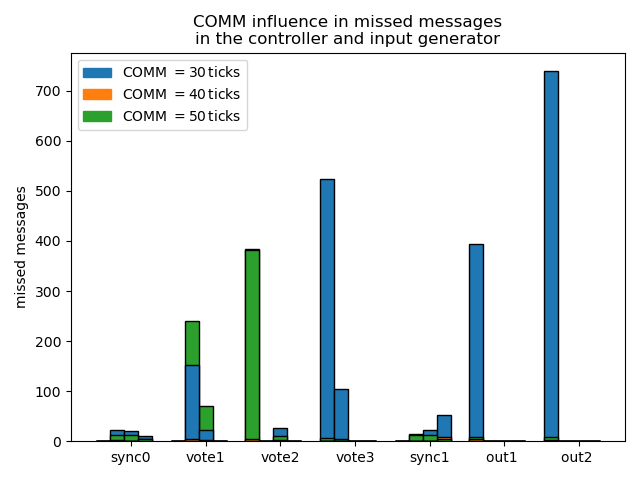
\includegraphics[width=\textwidth]{figures/missing_msgs/missed_msgs_COMM_ctrl.png}
         \caption{}
     \end{subfigure}
     \hfill
     \begin{subfigure}[b]{0.4\textwidth}
         \centering
         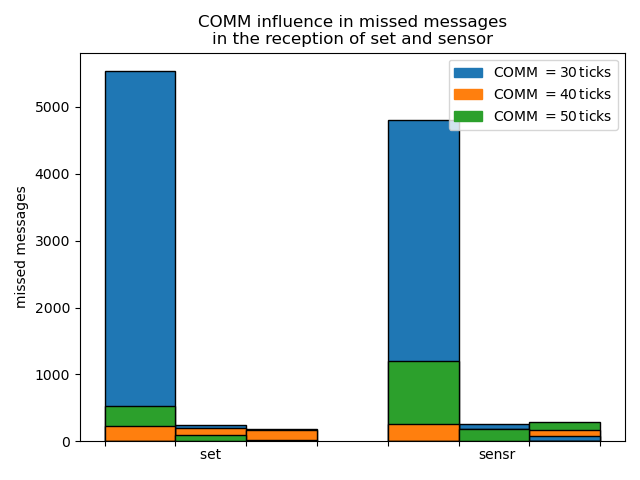
\includegraphics[width=\textwidth]{figures/missing_msgs/missed_msgs_COMM_set_sensr.png}
         \caption{}
     \end{subfigure}
     \hfill
     \begin{subfigure}[b]{0.4\textwidth}
         \centering
         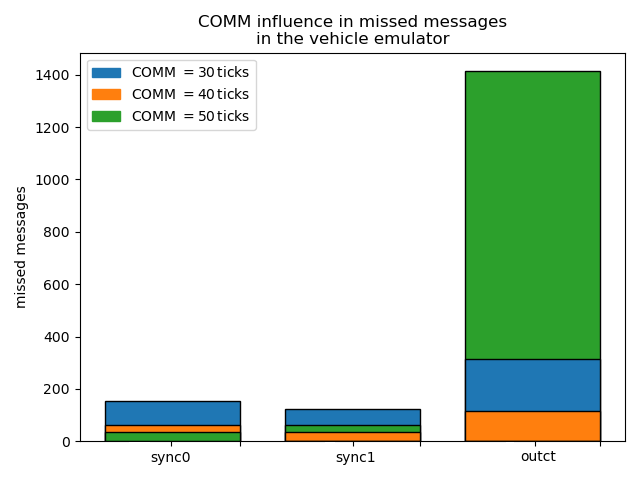
\includegraphics[width=\textwidth]{figures/missing_msgs/missed_msgs_COMM_vem.png}
         \caption{}
     \end{subfigure}
        \caption{Missed messages for every different board listening to each different message for different COMM values. (a) The controller and input generator listen to controller messages, (b) the controller listen to set and sensor messages and (c) the vehicle emulator listens to time master messages. Every board misses are represented by a bar for each message, from left to right, board$_1$, board$_2$, board$_3$, input generator and vehicle emulator.}
        \label{fig:mss_msgs_comm}
\end{figure}

In general, taking into account the variability from figure (\ref{fig:mss_msgs_var}), COMM = $30\,$ticks and COMM = $50\,$ticks present worse results than COMM = $40\,$ticks. It seems the maximum set load of seven copies per message presents a worse behaviour than sending some lower amount, as can be seen for the longest COMM period. For a shorter COMM period it is possible that the amount of copies sent per message is too low, so the chances of a missed message increase.\\

The next analysis focuses in the amount of copies sent during the same task. Figure (\ref{fig:mss_msgs_incr}) shows the missed messages for COMM = $30\,$ticks for two different transmitting frequency configurations. For $\phi_1 = 5\,$ticks, $\phi_2 = 8\,$ticks (the frequency chosen for the COMM measurement) the amount of messages per task is eight. For $\phi_1 = 3\,$ticks, $\phi_2 = 4\,$ticks the amount of messages per task is fourteen (the maximum allowed in the prototype).\\

\begin{figure}[h!]
     \centering
     \begin{subfigure}[b]{0.8\textwidth}
         \centering
         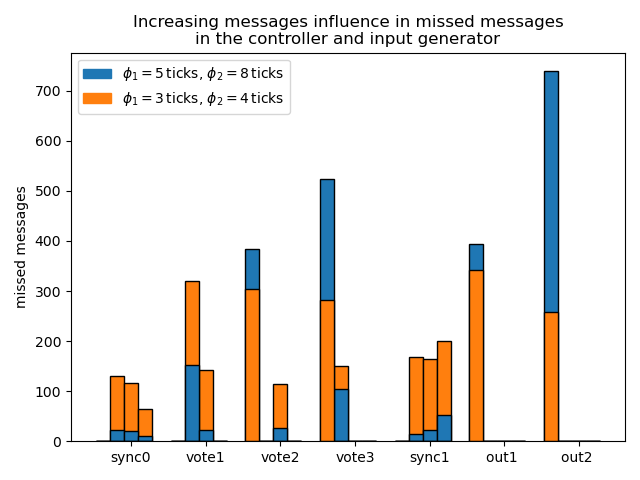
\includegraphics[width=\textwidth]{figures/missing_msgs/missed_msgs_IncrMsgs_ctrl.png}
         \caption{}
     \end{subfigure}
     \hfill
     \begin{subfigure}[b]{0.4\textwidth}
         \centering
         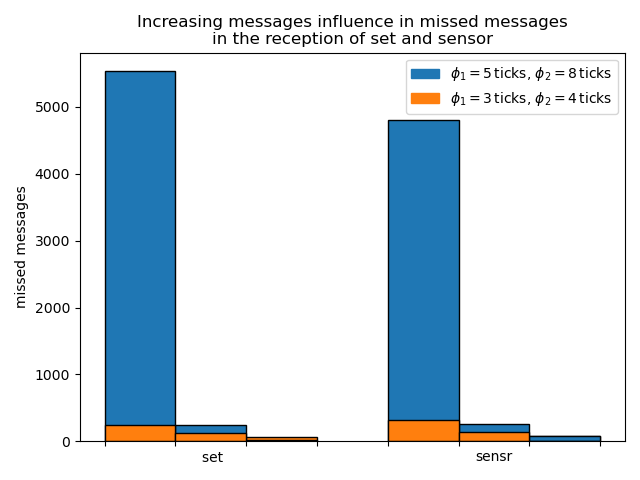
\includegraphics[width=\textwidth]{figures/missing_msgs/missed_msgs_IncrMsgs_set_sensr.png}
         \caption{}
     \end{subfigure}
     \hfill
     \begin{subfigure}[b]{0.4\textwidth}
         \centering
         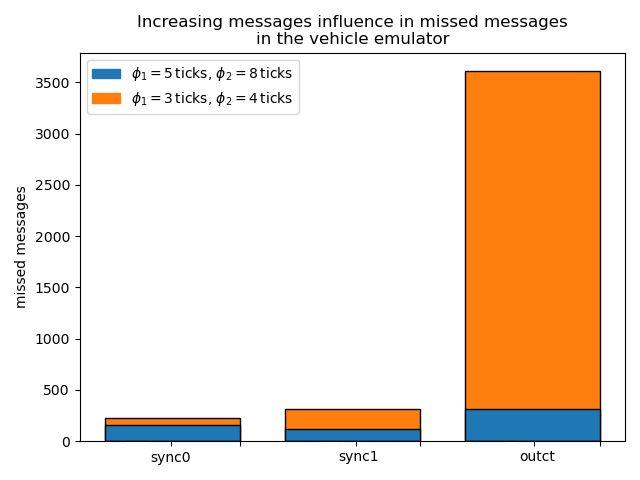
\includegraphics[width=\textwidth]{figures/missing_msgs/missed_msgs_IncrMsgs_vem.png}
         \caption{}
     \end{subfigure}
        \caption{Missed messages for every different board listening to each different message for two different transmitting frequencies. (a) The controller and input generator listen to controller messages, (b) the controller listen to set and sensor messages and (c) the vehicle emulator listens to time master messages. Every board misses are represented by a bar for each message, from left to right, board$_1$, board$_2$, board$_3$, input generator and vehicle emulator.}
        \label{fig:mss_msgs_incr}
\end{figure}

Sending more copies of the same message does not seem to improve the performance in general. However, it is interesting to see how for a lower amount of messages the reception at the controller for the set and sensor messages is better, while for a higher amount of copies the reception at the vehicle emulator for the outctrl message is better.\\

The last configuration explored tries to set a message frequency and baud rate couple that avoids message clashing in the network. According to \citep{CAN_bitrate}, lower baud rates are more robust. Also, waiting until the last message sent has arrived at its destination could help in CAN management during a communication task, resulting in a lower missing rate. With baud rate = $1\,$Mbit/s a total of $4000\,$bits can be transmitted during a COMM = $40\,$ticks communication task. Baud rates of $500\,$kbit/s and $250\,$kbit/s has been used for COMM = $50\,$ticks, which allow for $1250\,$bits and $2500\,$bits, respectively. Assuming a worst case scenario of 130 bits per message frame in its copy transmission, as presented in \citep{busload_question}, there is no case in which the maximum of seven sent copies is over the capabilities of the network. When checking the communication delay for different baud rates, $3\,$ticks delay was found for $1\,$Mbit/s, $5\,$ticks for $500\,$kbit/s and $7\,$ticks for $250\,$kbit/s. At least, these amounts of ticks have been set from one copy to the next in the transmission for the measurements presented in figure (\ref{fig:mss_msgs_clash}). The message phases chosen are $\phi_{init2} = 5\,$ticks, $\phi_1 = \phi_2 = 10\,$ticks for COMM = $40\,$ticks and baud rate $1\,$Mbit/s, $\phi_{init2} = 5\,$ticks, $\phi_1 = \phi_2 = 10\,$ticks for COMM = $50\,$ticks and baud rate $500\,$kbit/s, $\phi_{init2} = 8\,$ticks, $\phi_1 = \phi_2 = 16\,$ticks for COMM = $50\,$ticks and baud rate $250\,$kbit/s.

\begin{figure}[h!]
     \centering
     \begin{subfigure}[b]{0.8\textwidth}
         \centering
         \includegraphics[width=\textwidth]{figures/missing_msgs/missed_msgs_Clash_ctrl.png}
         \caption{}
     \end{subfigure}
     \hfill
     \begin{subfigure}[b]{0.4\textwidth}
         \centering
         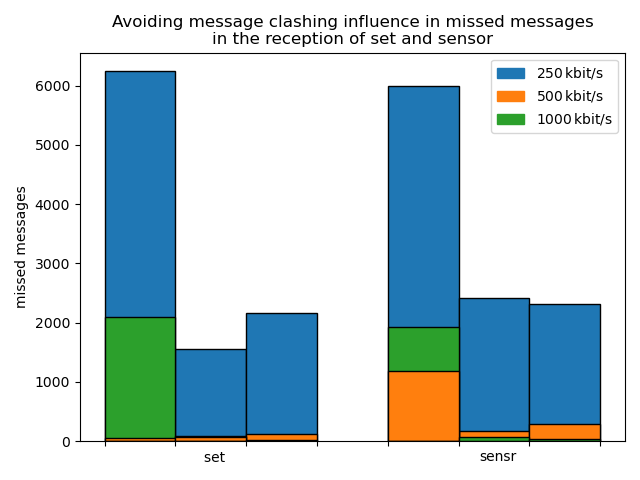
\includegraphics[width=\textwidth]{figures/missing_msgs/missed_msgs_Clash_set_sensr.png}
         \caption{}
     \end{subfigure}
     \hfill
     \begin{subfigure}[b]{0.4\textwidth}
         \centering
         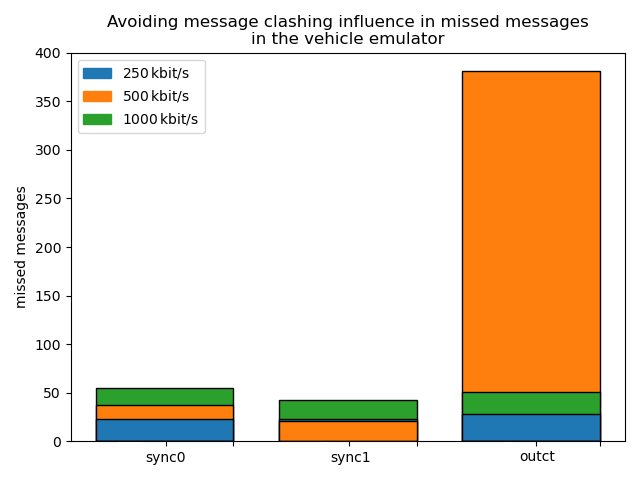
\includegraphics[width=\textwidth]{figures/missing_msgs/missed_msgs_Clash_vem.png}
         \caption{}
     \end{subfigure}
        \caption{Missed messages for every different board listening to each different message for three avoiding message clash configurations. (a) The controller and input generator listen to controller messages, (b) the controller listen to set and sensor messages and (c) the vehicle emulator listens to time master messages. Every board misses are represented by a bar for each message, from left to right, board$_1$, board$_2$, board$_3$, input generator and vehicle emulator.}
        \label{fig:mss_msgs_clash}
\end{figure}

When looking at the results for avoiding message clashing in the network, there is not a noticeable difference when measuring at COMM = $40\,$ticks with respect to the results when sending the messages without avoiding message clashing. With lower baud rate the reception of the messages set and sensor by the controller is unstable but the reception of outctrl at the vehicle emulator is very good. The opposite happens for baud rate $500\,$kbit/s.

\subsection{Conclusions}
With the current data it is not possible to assess a perfect scenario where the missing messages is almost zero. However, it is possible to see some negative correlation between the reception of the messages set and sensor received by the controller boards and the message outctrl received by the vehicle emulator. When there is a low load of copies per message or the baud rate is $250\,$kbit/s the reception of the messages set and sensor is unstable at the controller but the message outctrl is received well by the vehicle emulator. The situation gets reversed when there is a high load of copies per message or the baud rate is $500\,$kbit/s. The best configuration found is the presented for figure (\ref{fig:mss_msgs_var}).


\end{document}